

\section{Выбор средств программной реализации}

\subsection{Язык программирования}
В качестве языка программирования был выбран Python 3\cite{python_doc}, по следующим причинам.
\begin{itemize}
	\item Поддержка ООП, требуемого для архитектурного шаблона MVC.
	\item Наличие опыта работы с данным языком.
	\item Данный язык является популярным в разработке web-приложений, поэтому он обладает большим количеством web-фреймворков и библиотек для доступа к СУБД.
\end{itemize}

\subsection{СУБД и ORM}
Наиболее популярными реляционными СУБД являются Oracle, MySQL и PostgreSQL\cite{dbm_source}. Их сравнение\cite{dbm_source2} можно свести в таблицу \ref{dms_table2}

\begin{center}
\begin{longtable}[h]{| p{2.4cm} | p{6.6cm} | p{6.6cm} |}
	\caption{Сравнение реляционных СУБД} \label{dms_table2} \\
 	\hline 
	\multicolumn{1}{|c|}{\textbf{СУБД}} &
	\multicolumn{1}{c|}{\textbf{Преимущества}} &
	\multicolumn{1}{c|}{\textbf{Недостатки}} \\
	\hline
	\endfirsthead
	
	\multicolumn{3}{c}%
	{{\tablename\ \thetable{} -- продолжение}} \\
 	\hline 
	\multicolumn{1}{|c|}{\textbf{СУБД}} &
	\multicolumn{1}{c|}{\textbf{Преимущества}} &
	\multicolumn{1}{c|}{\textbf{Недостатки}} \\
	\hline
	\endhead
	
	\hline \multicolumn{3}{|r|}{{Продолжение на следующей странице}} \\ \hline
	\endfoot
	
	\hline
	\endlastfoot
	
	\hline
	Oracle		&	+ надёжность системы	& -	конечная стоимость СУБД	\\ 
	&	+ поддержка современности функционала	& - высокие системные требования \\ 
	\hline
	
	
	MySQL	&	+ прост в установке и использовании	& -	проблемы с надёжностью	\\ 
	&	+ производительность	& - не полная поддержка SQL \\ 
	&	+ широкий базовый функционал & \\
	\hline
	
	PostgreSQL	&	+ лёгкая масштабируемость	& -	низкая скорость выполнения пакетных операций	\\ 
	&	+ открытость ПО	& - сложности поиска хостинга \\ 
	&	+ поддержка текстовых форматов (в т.ч. json) & \\
\end{longtable}
\end{center}

Наиболее подходящим для небольших организаций, которые являются целевыми для разрабатываемой программы, является PostgreSQL\cite{dbm_source2}. Учитывая наличие опыта работы с данным средством, оно был выбран в качестве СУБД для данного курсового проекта.

В качестве ORM (технология объектно-реляционного преобразования) был выбран peewee\cite{peewee_doc}, так как она является простой в освоении и использовании, а также позволяет легко подменять СУБД.

\subsection{Web-фреймворк}
В качестве web-фреймворка был выбран Django\cite{django_doc}, по следующим причинам.
\begin{itemize}
	\item Django использует шаблон проектирования MVC.
	\item Лёгкая масштабируемость.
	\item Готовые решения для наиболее востребованных задач.
	\item Поддержка шаблонизации html страниц.
\end{itemize}


\newpage
\section{UML-диаграммы компонентов приложения}
\subsection{Компонент доступа к данным}
В данной работе компонент доступа к данным реализован с использованием паттерна проектирования Repository. UML диаграмма компонента изображена представленна на рисунке \ref{rep_pic} 

\begin{figure}[h!] 
	\begin{center}
%		{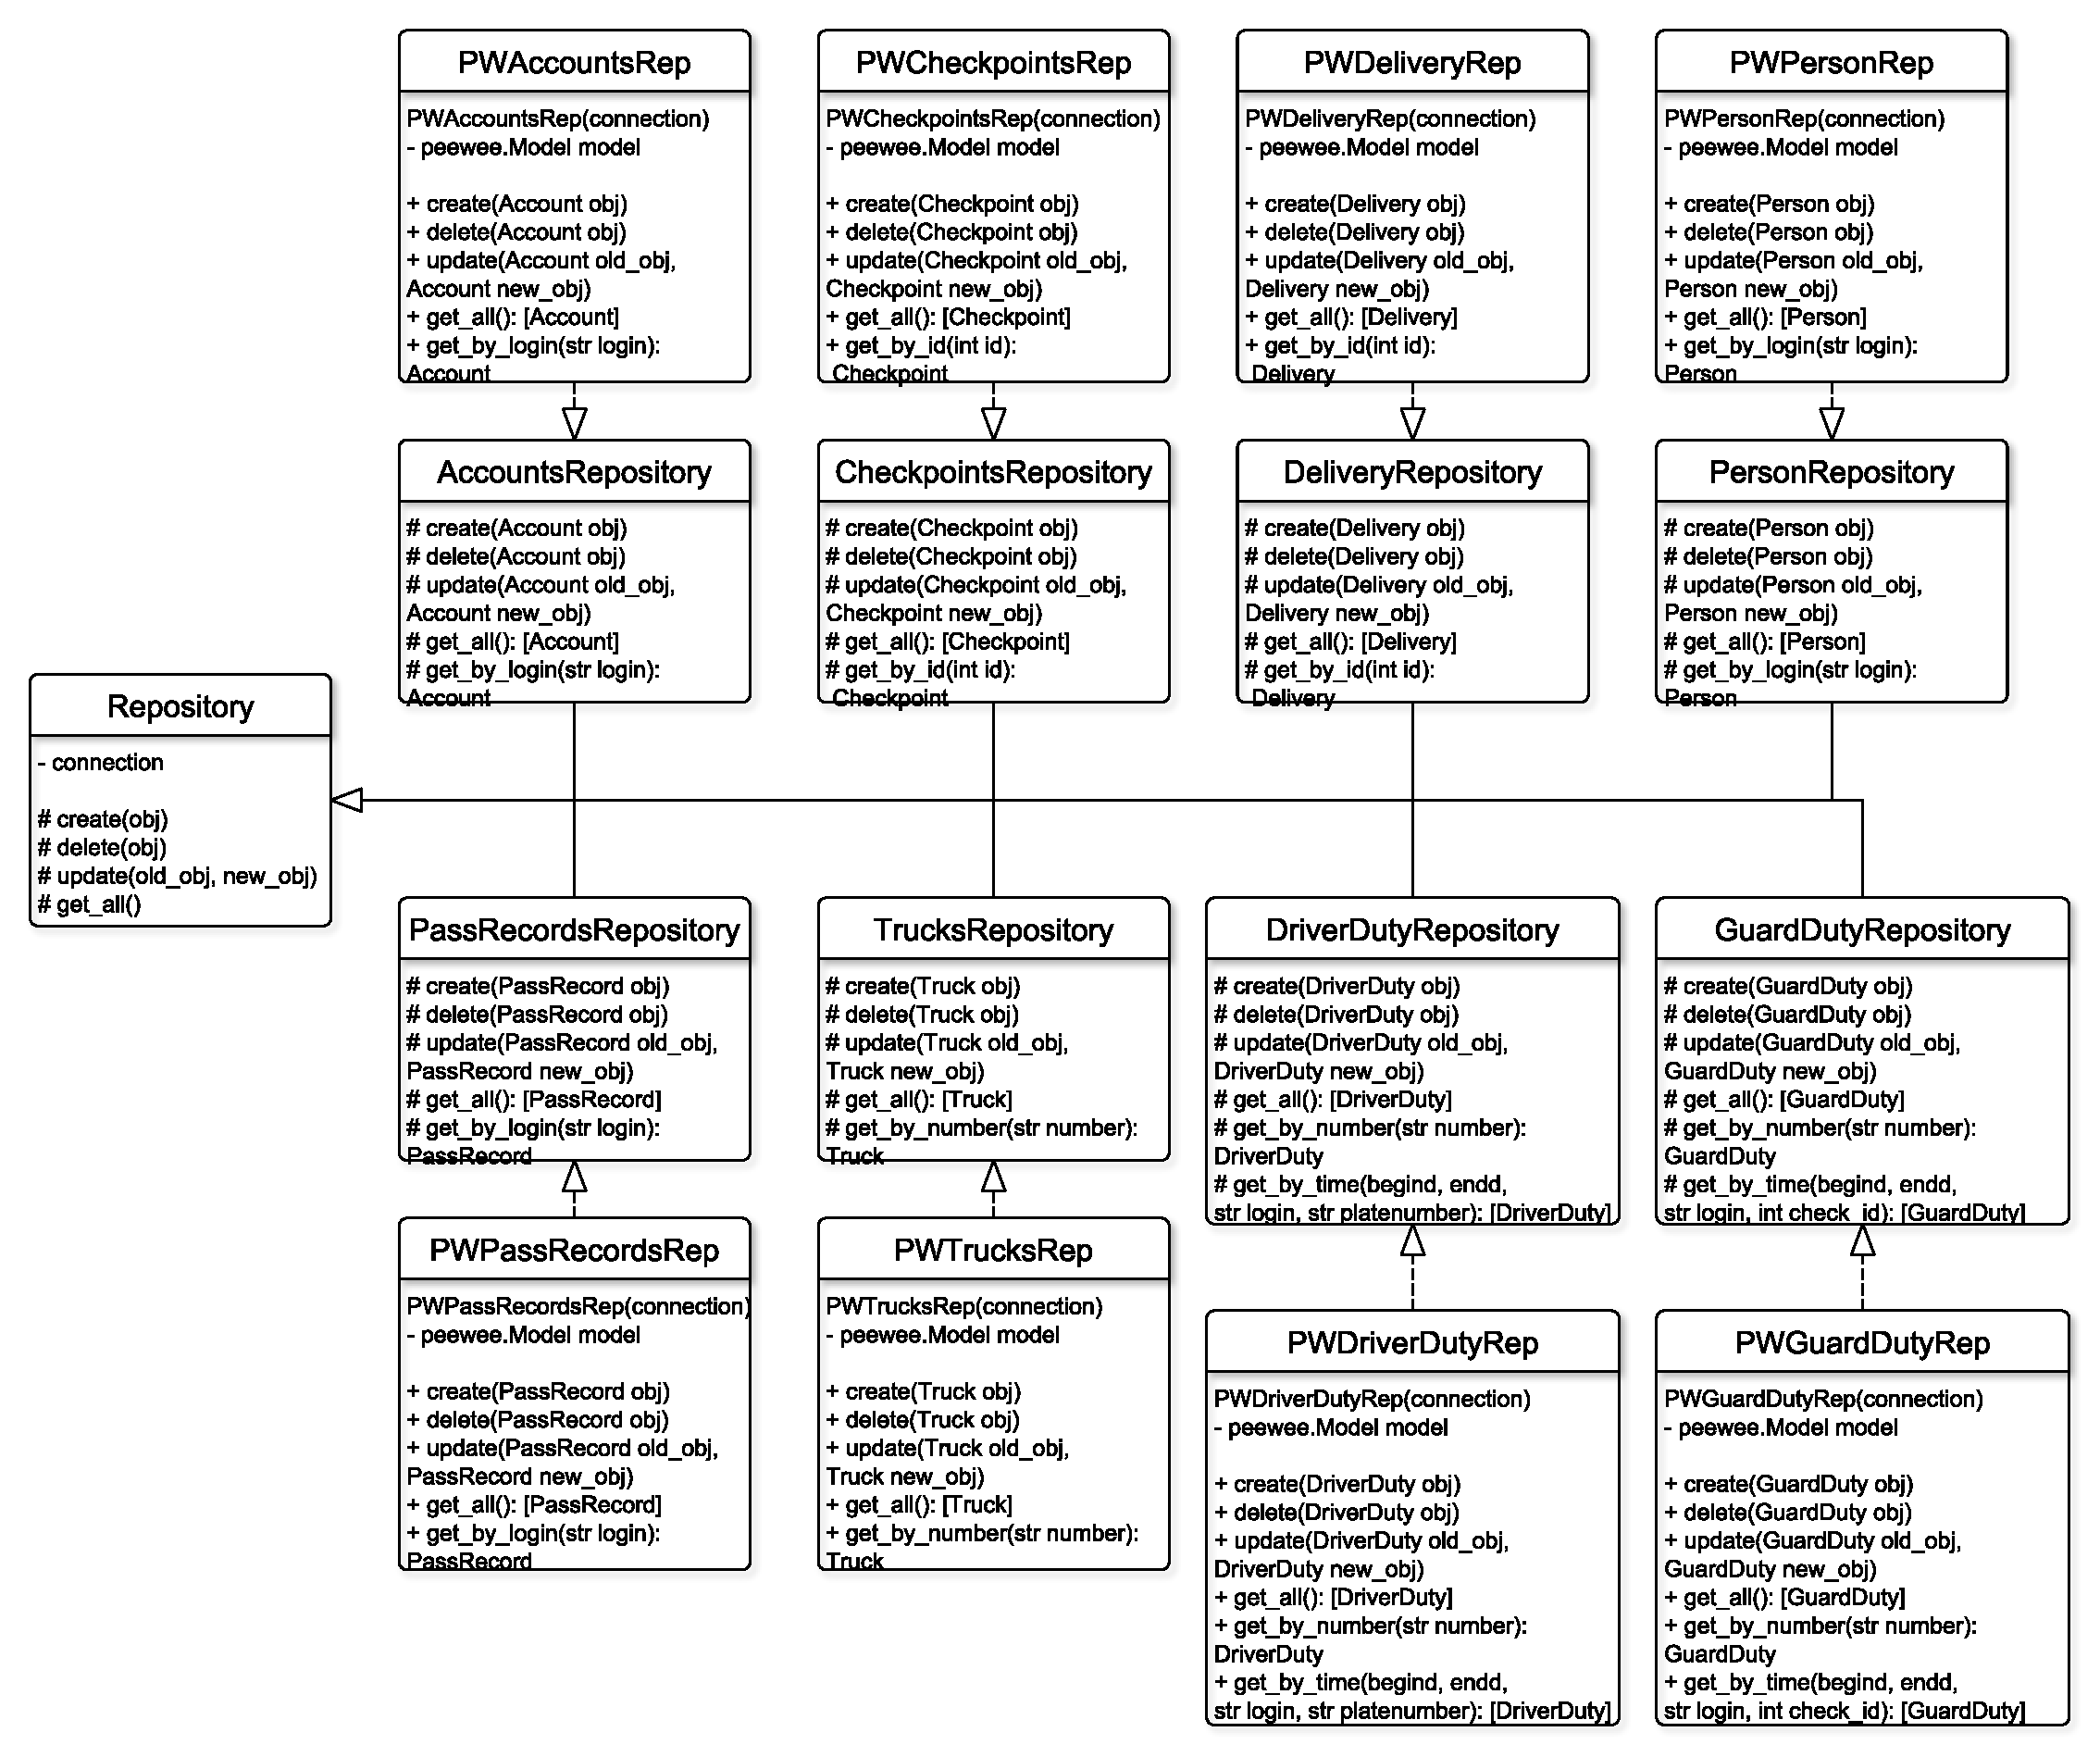
\includegraphics[height=14cm, width = 14cm]{uml/repsoitory.pdf}}
		{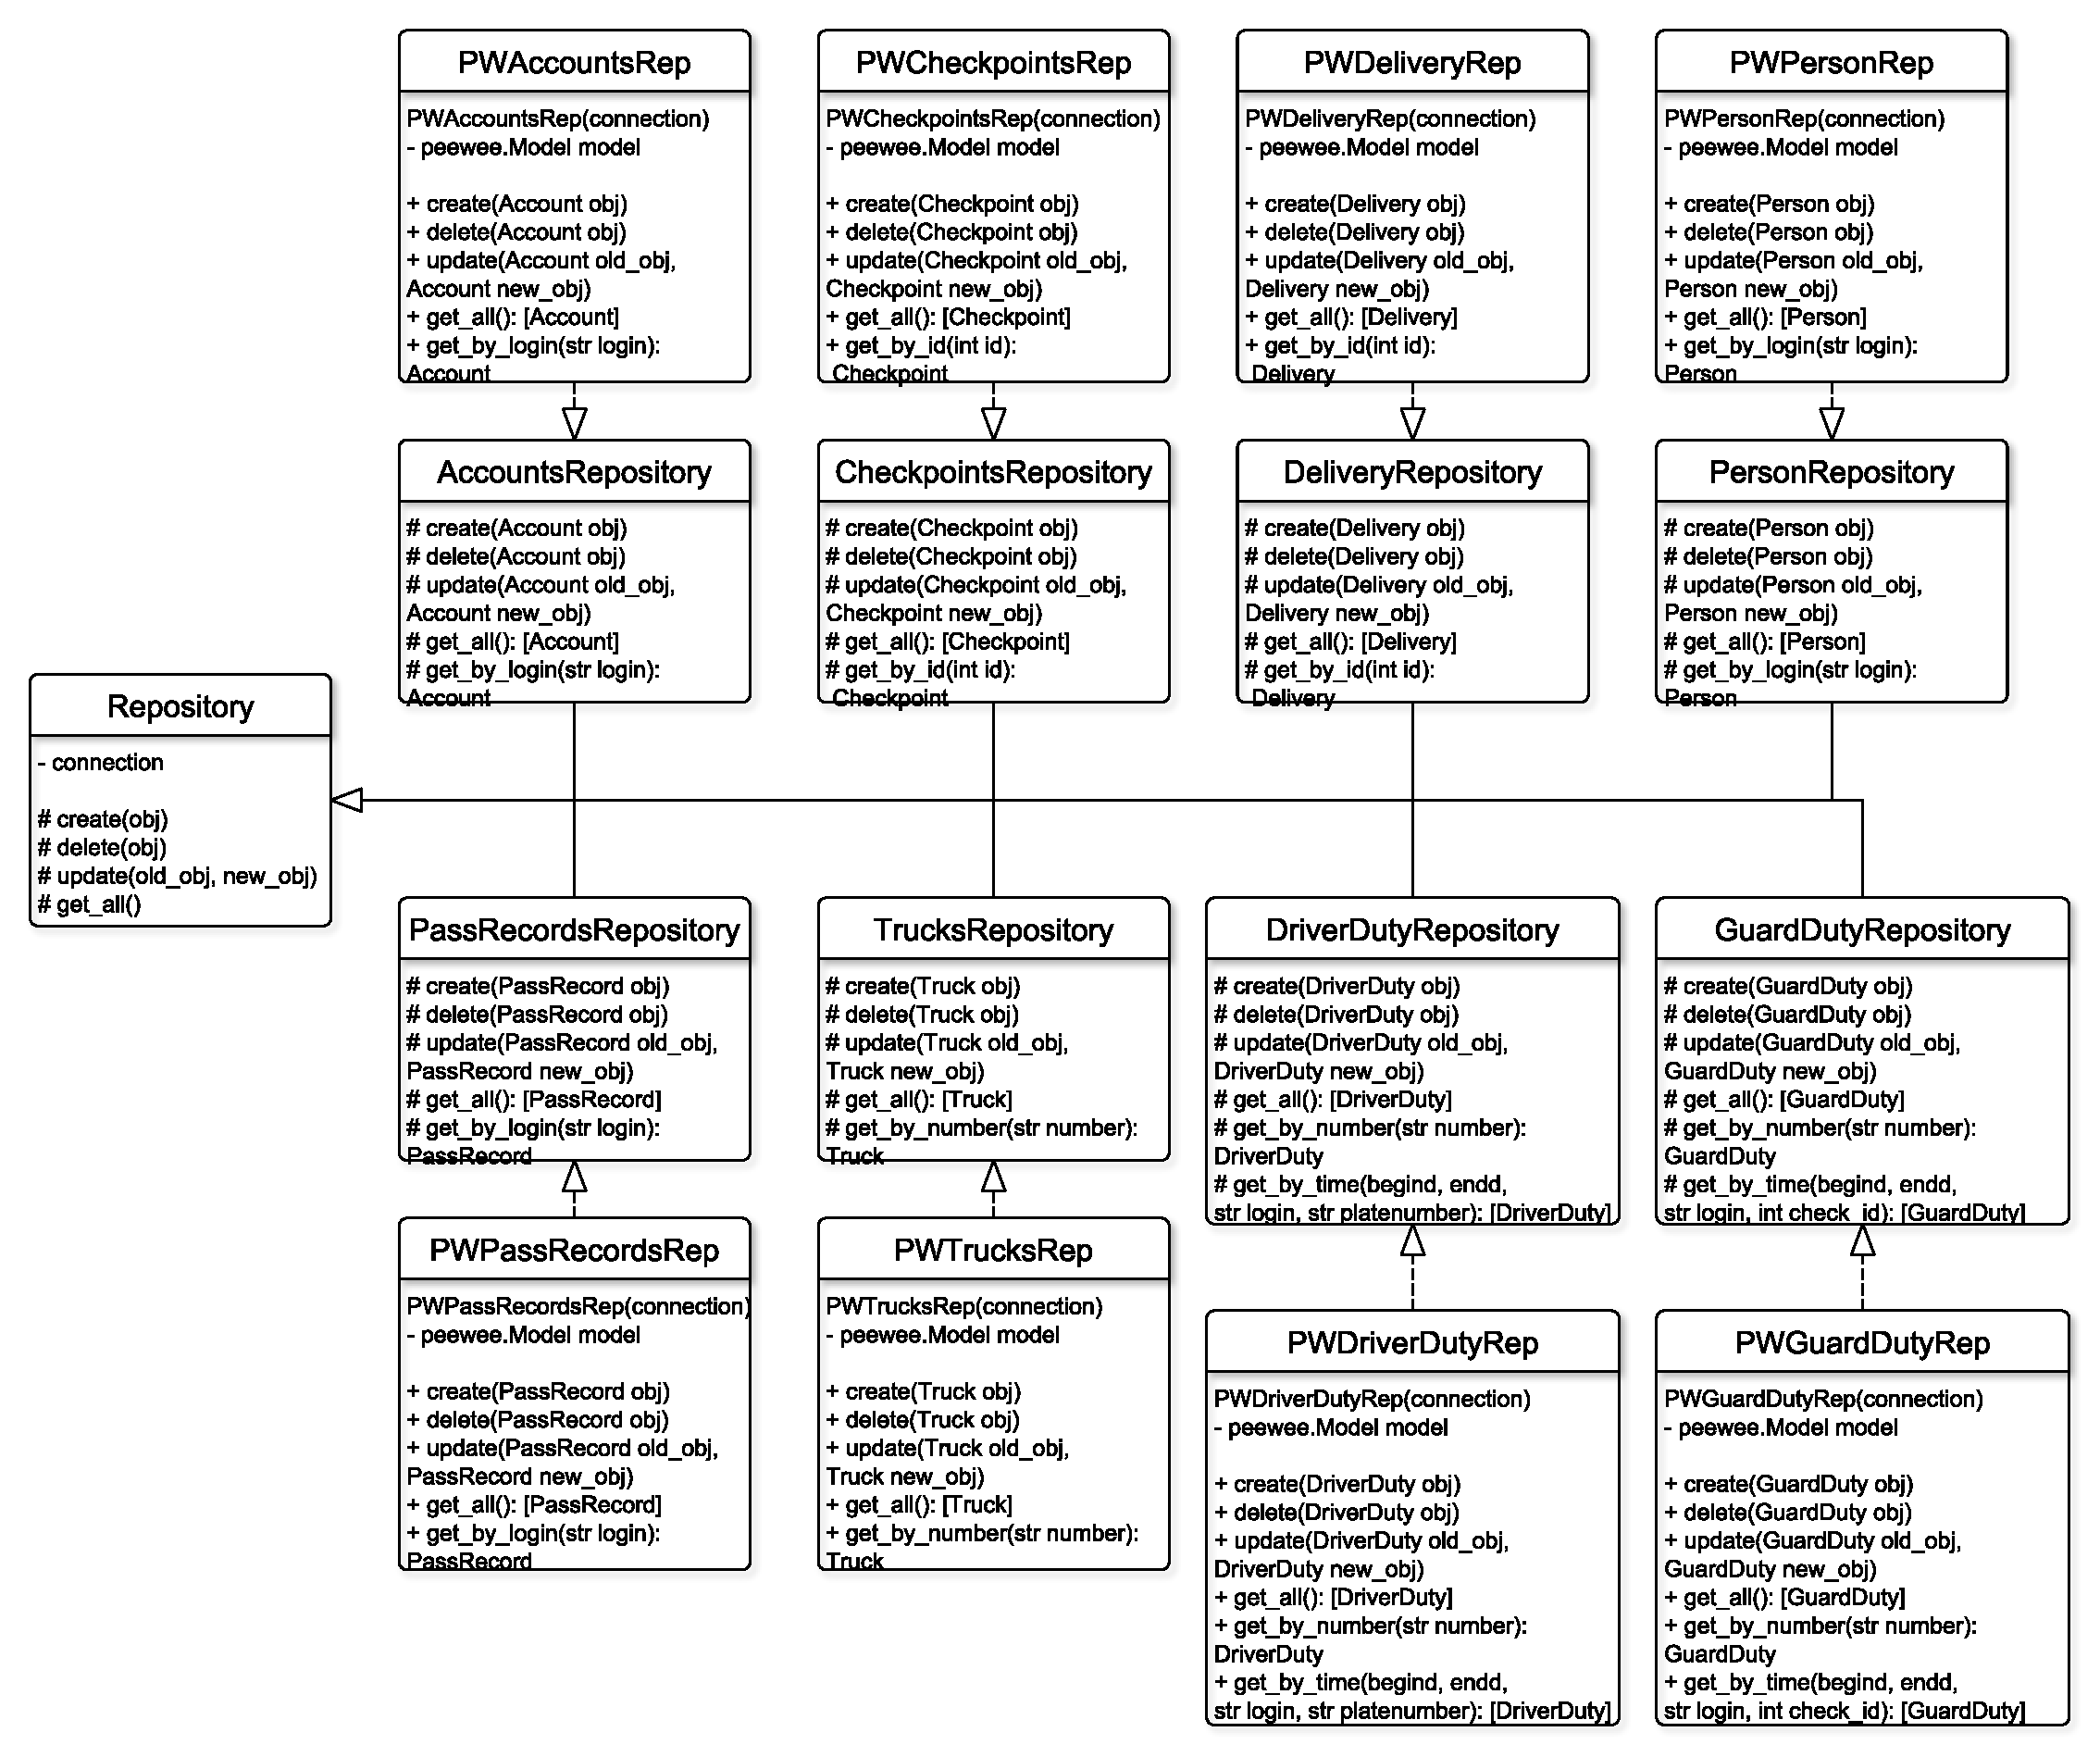
\includegraphics[scale=0.4, angle=0]{uml/repsoitory.pdf}}
		\caption{UML-диаграмма компонента доступа к данным}
		\label{rep_pic}
	\end{center}
\end{figure}

\newpage
\subsection{Компонент бизнес-логики}
В соответствии с подходом MVC был создан компонент бизнес-логики, выполняющий основную обработку данных, UML диаграмма которого представленна на рисунке \ref{model_pic}

\begin{figure}[h!] 
	\begin{center}
		%		{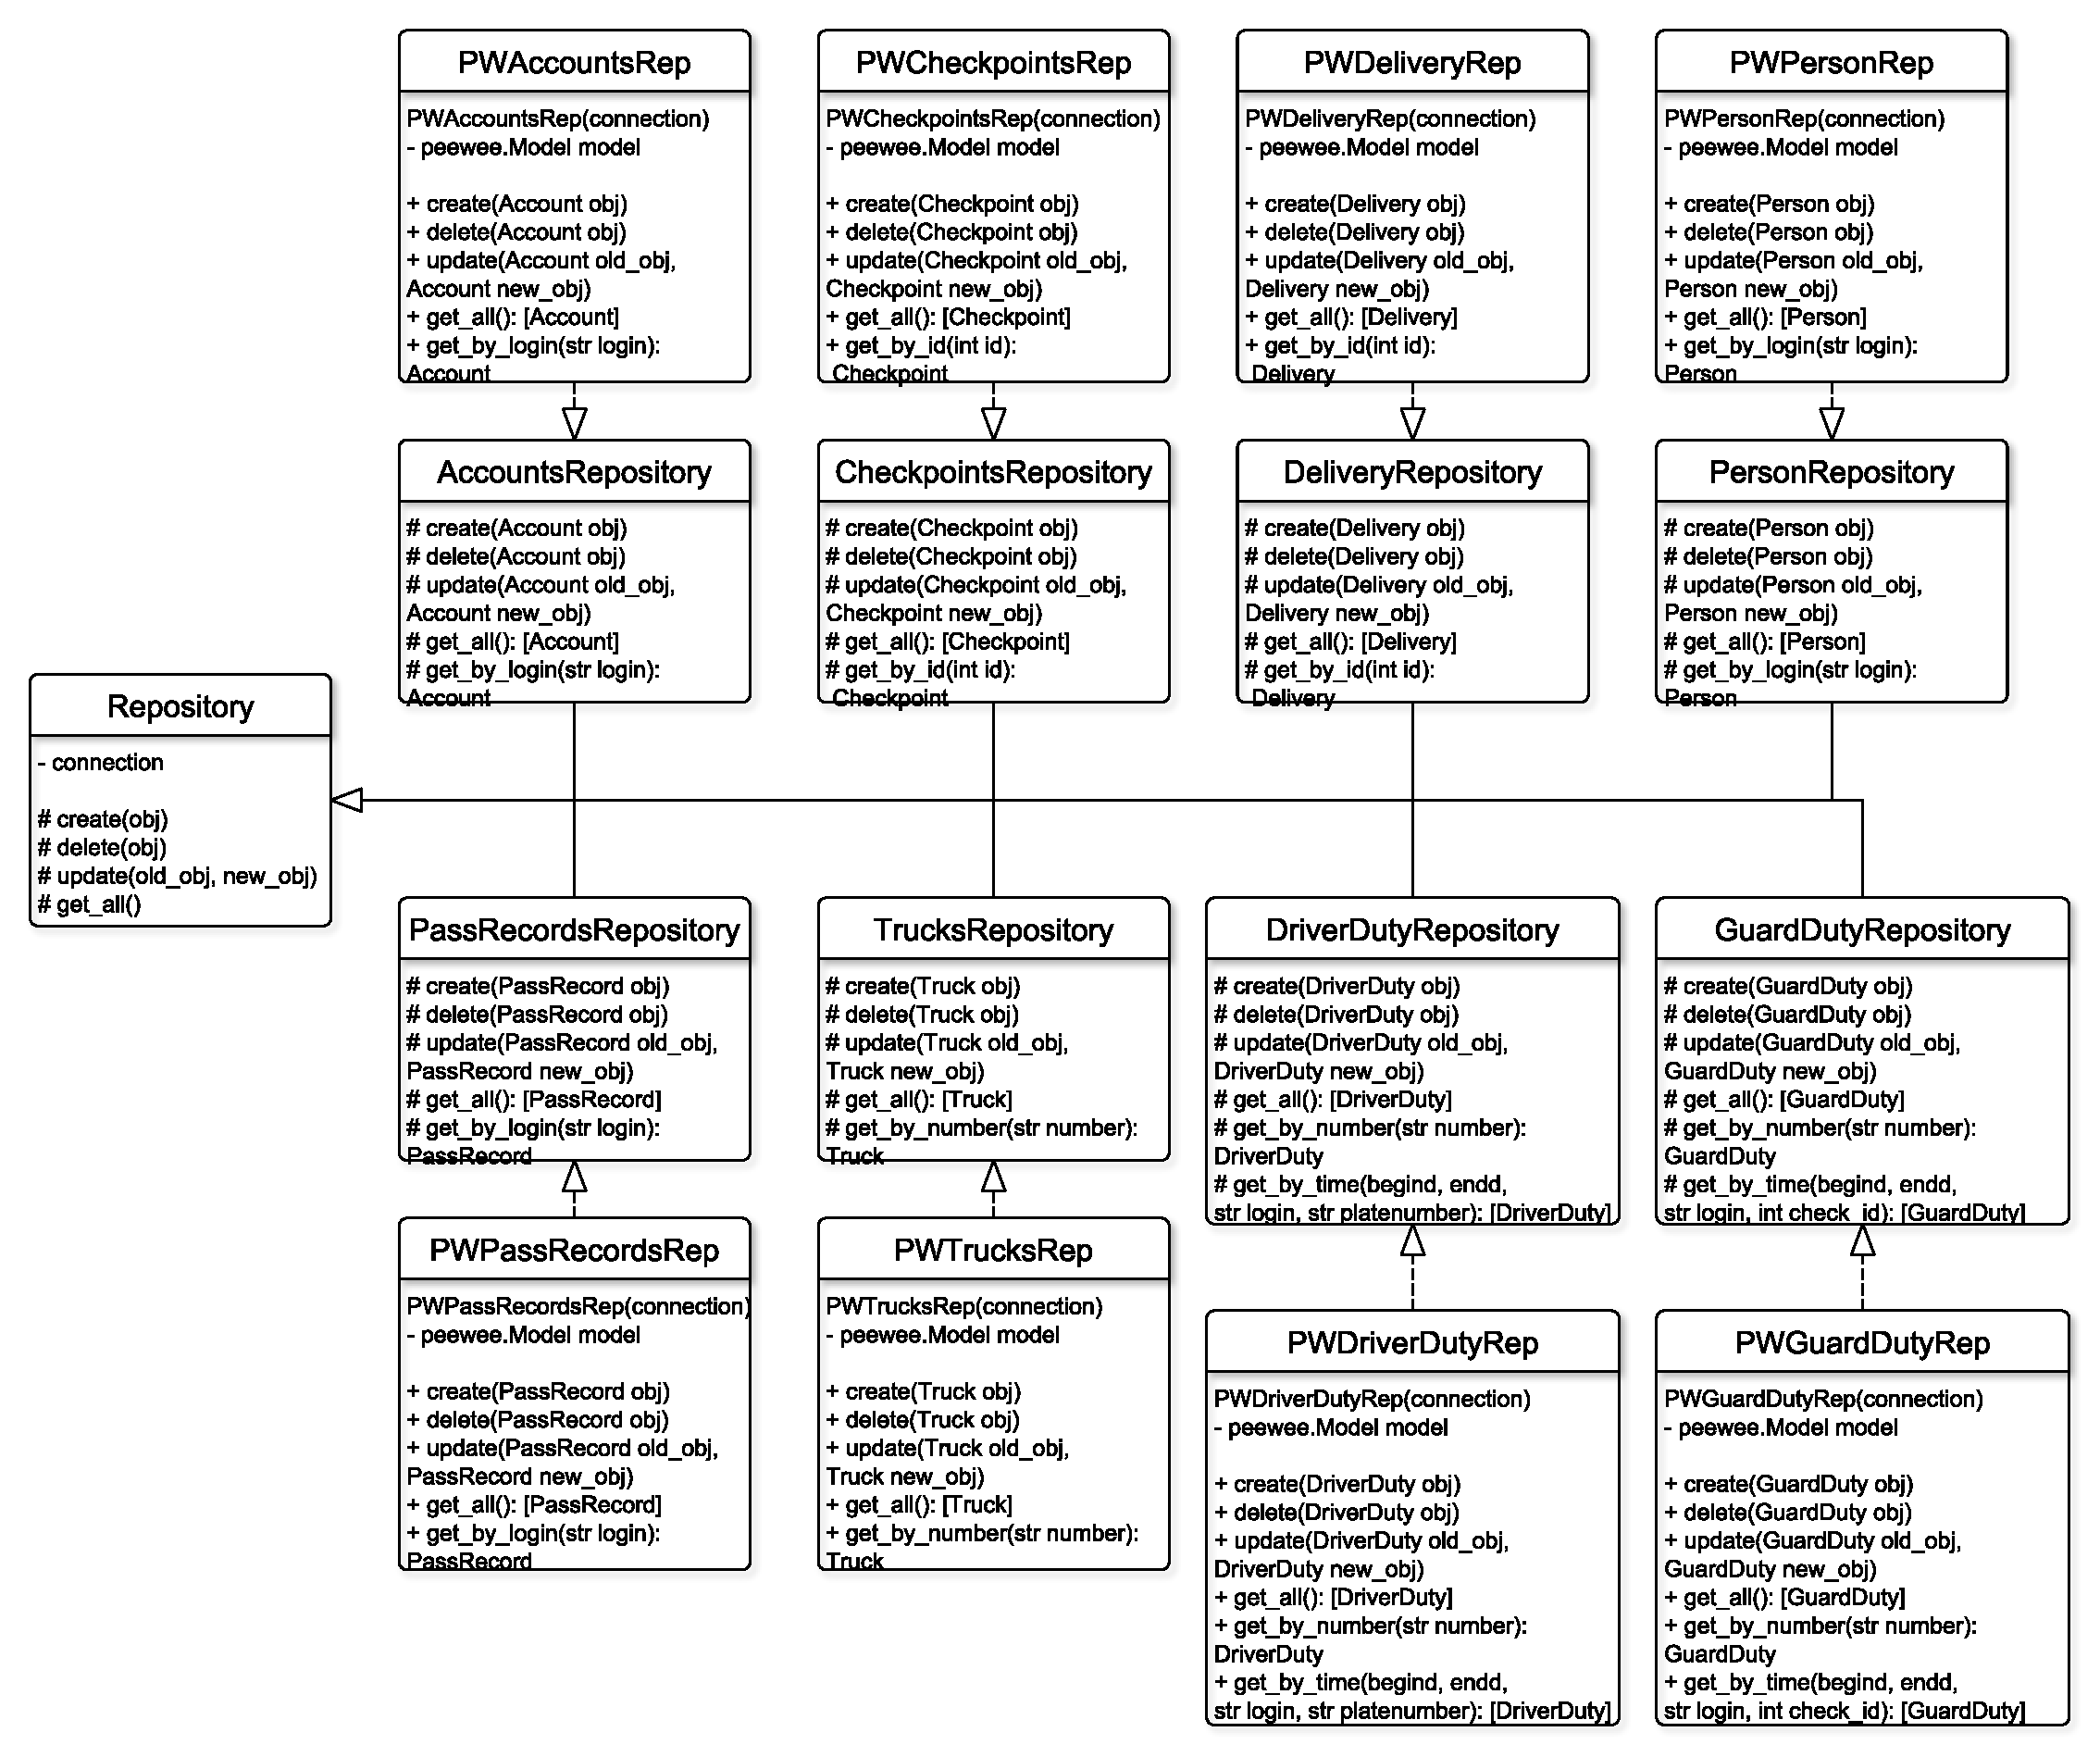
\includegraphics[height=14cm, width = 14cm]{uml/repsoitory.pdf}}
		{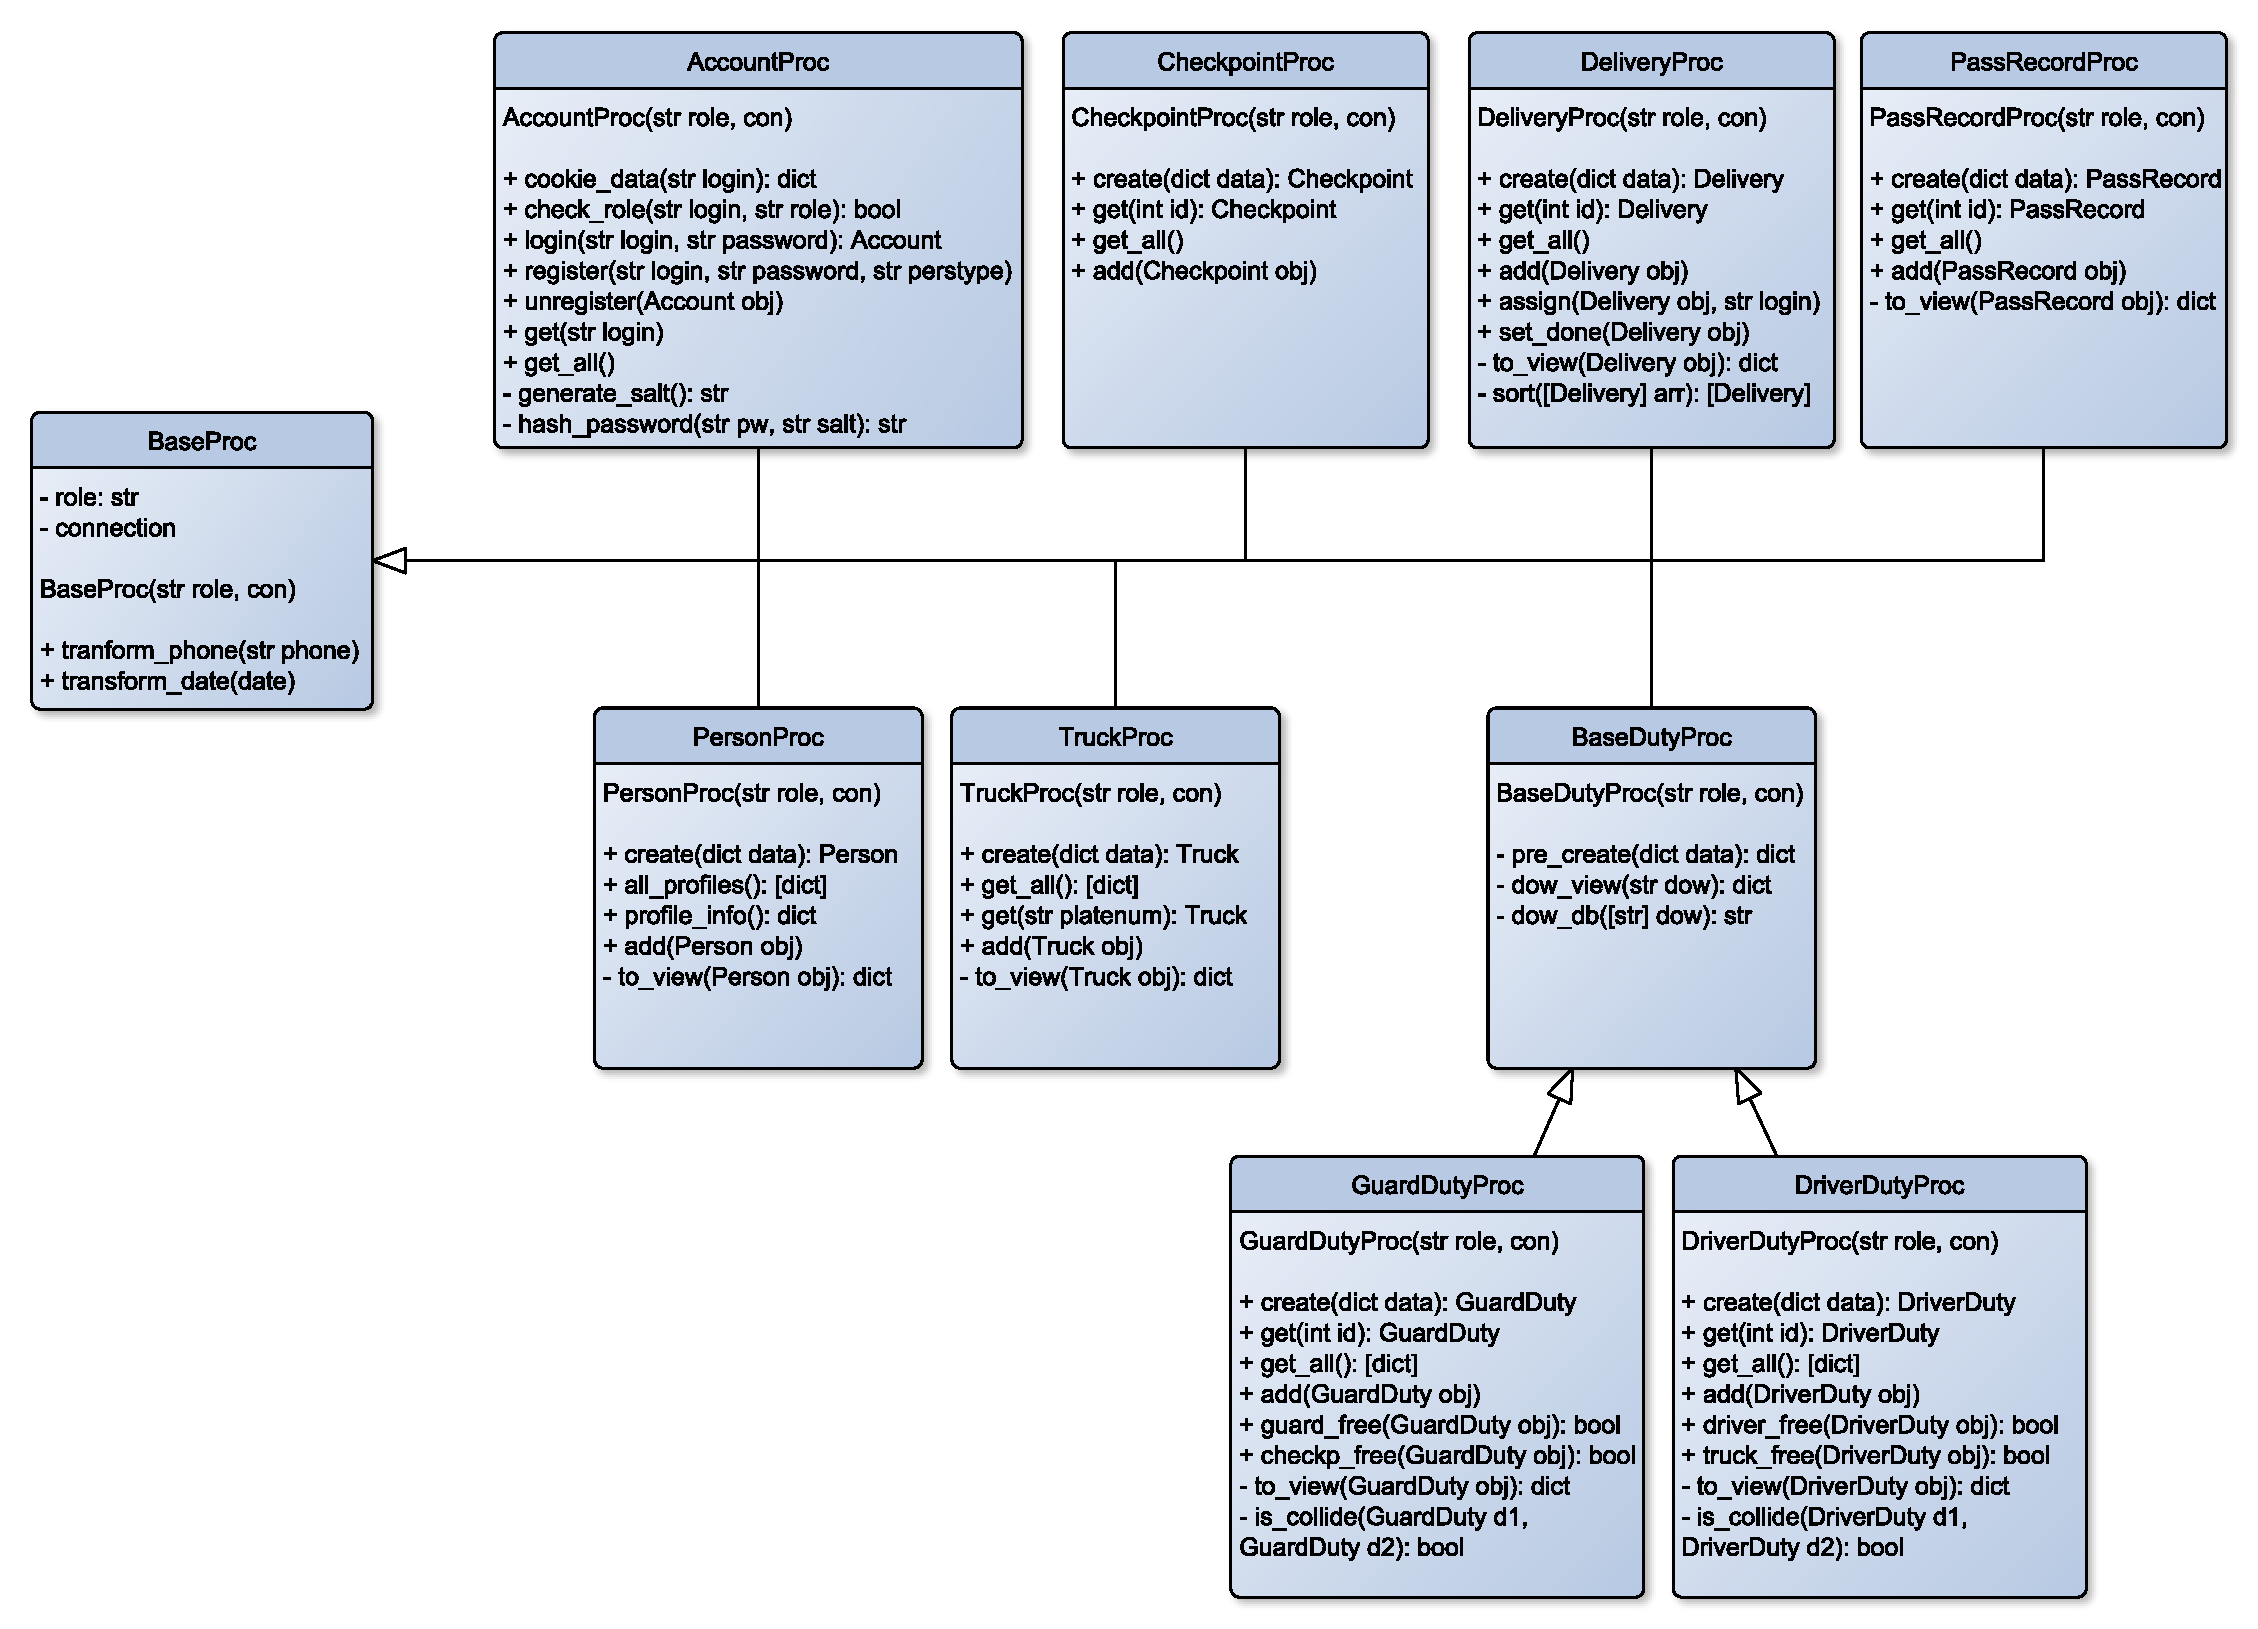
\includegraphics[scale=0.5, angle=0]{uml/business_models.pdf}}
		\caption{UML-диаграмма компонента бизнес-логики}
		\label{model_pic}
	\end{center}
\end{figure}

\newpage
\subsection{Компонент представления}
Также создан компонент представления, выполняющий отображение web-страниц в ответ на запросы пользователя, UML диаграмма которого представленна на рисунке \ref{view_pic}. Помимо этого был реализован технический компонент представления, отображающий информацию в символьном виде, для возможности тестирования компонента бизнес-логики.

\begin{figure}[h!] 
	\begin{center}
		%		{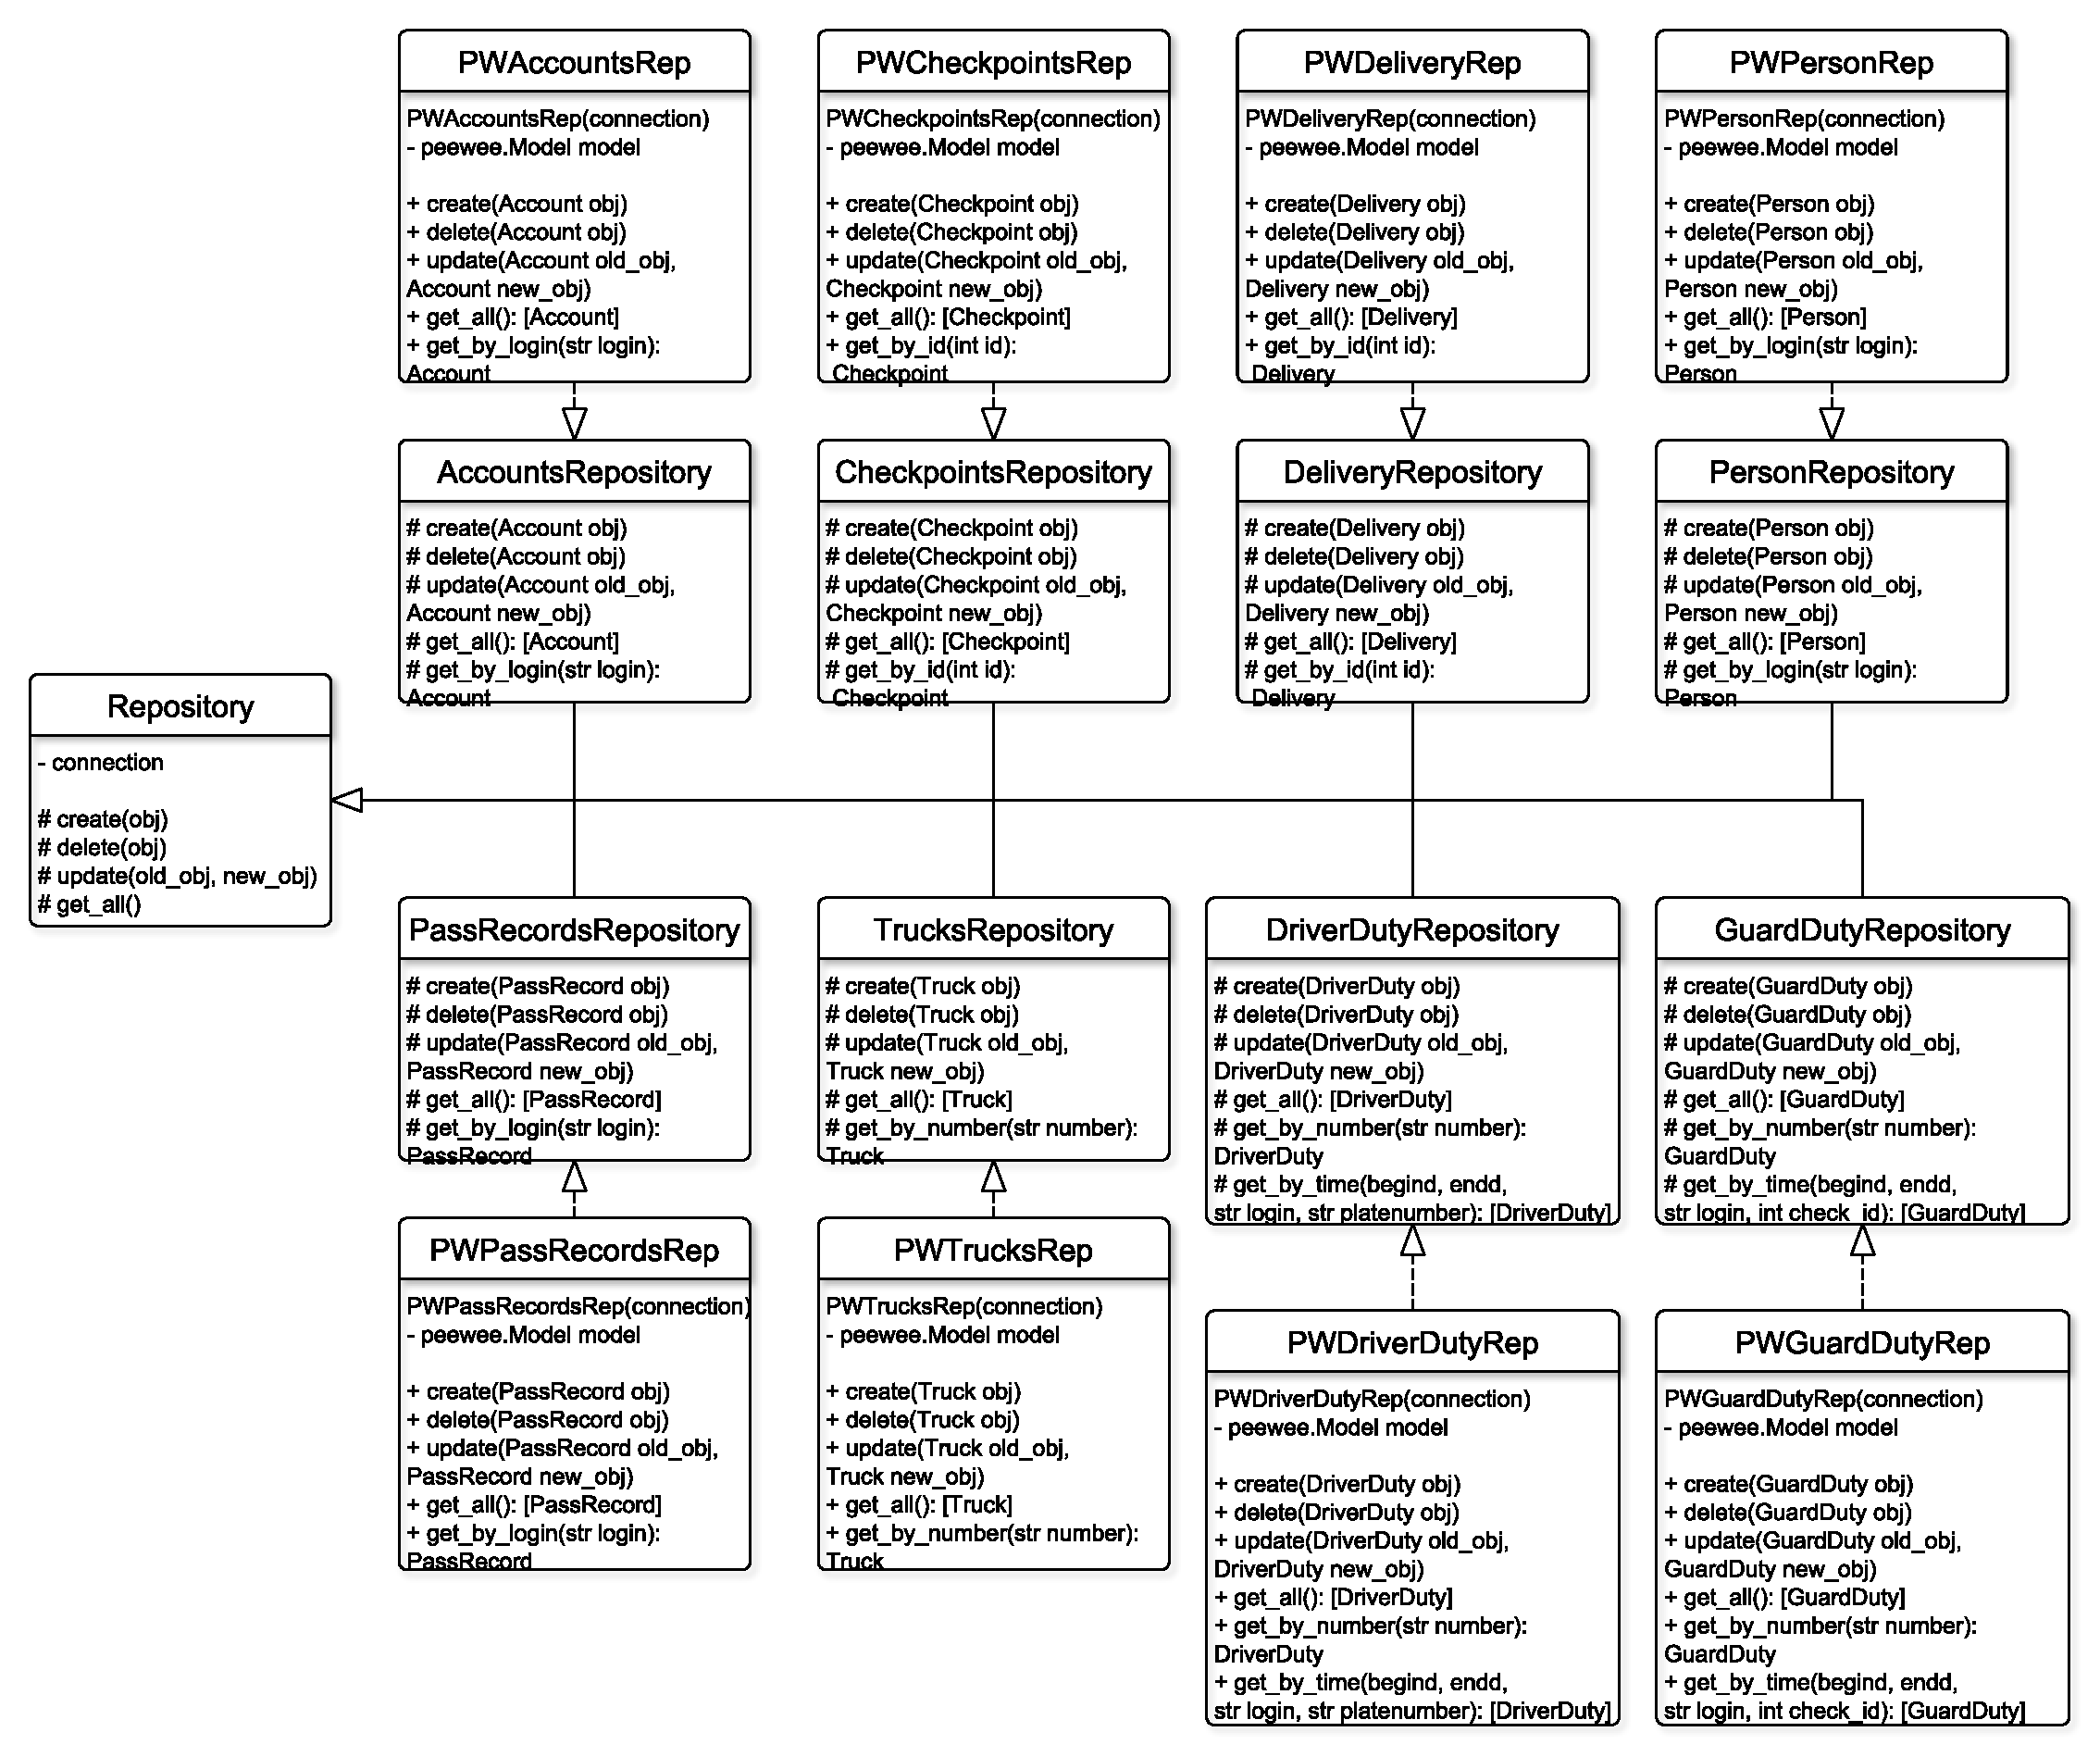
\includegraphics[height=14cm, width = 14cm]{uml/repsoitory.pdf}}
		{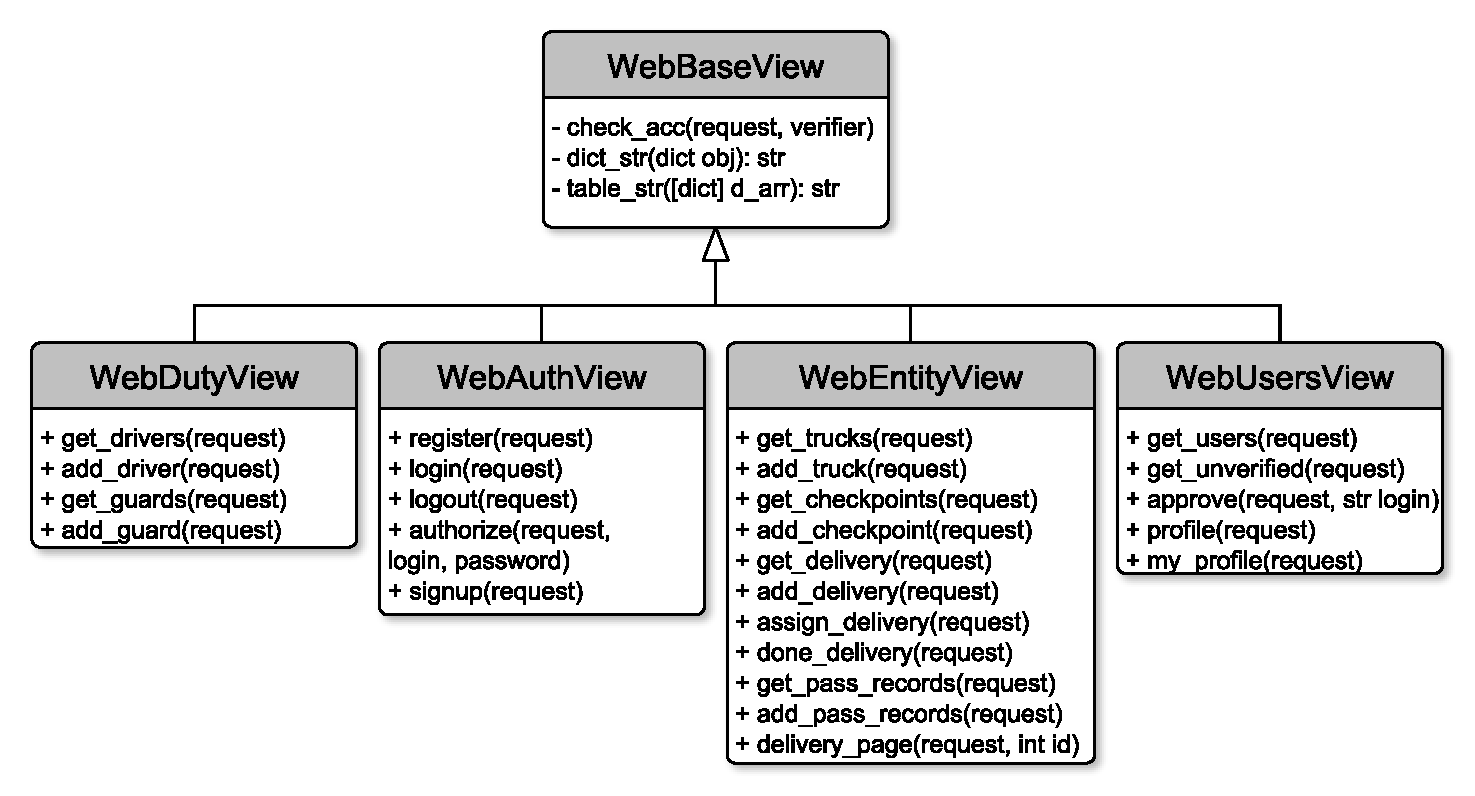
\includegraphics[scale=0.5, angle=0]{uml/webGUI.pdf}}
		\caption{UML-диаграмма компонента web-представления}
		\label{view_pic}
	\end{center}
\end{figure}

\newpage
\subsection{Диаграмма приложения}
Все перечисленные компоненты можно объединить в одну UML-диаграмму всего приложения на рисунке \ref{alluml_pic}

\begin{figure}[h!] 
	\begin{center}
		%		{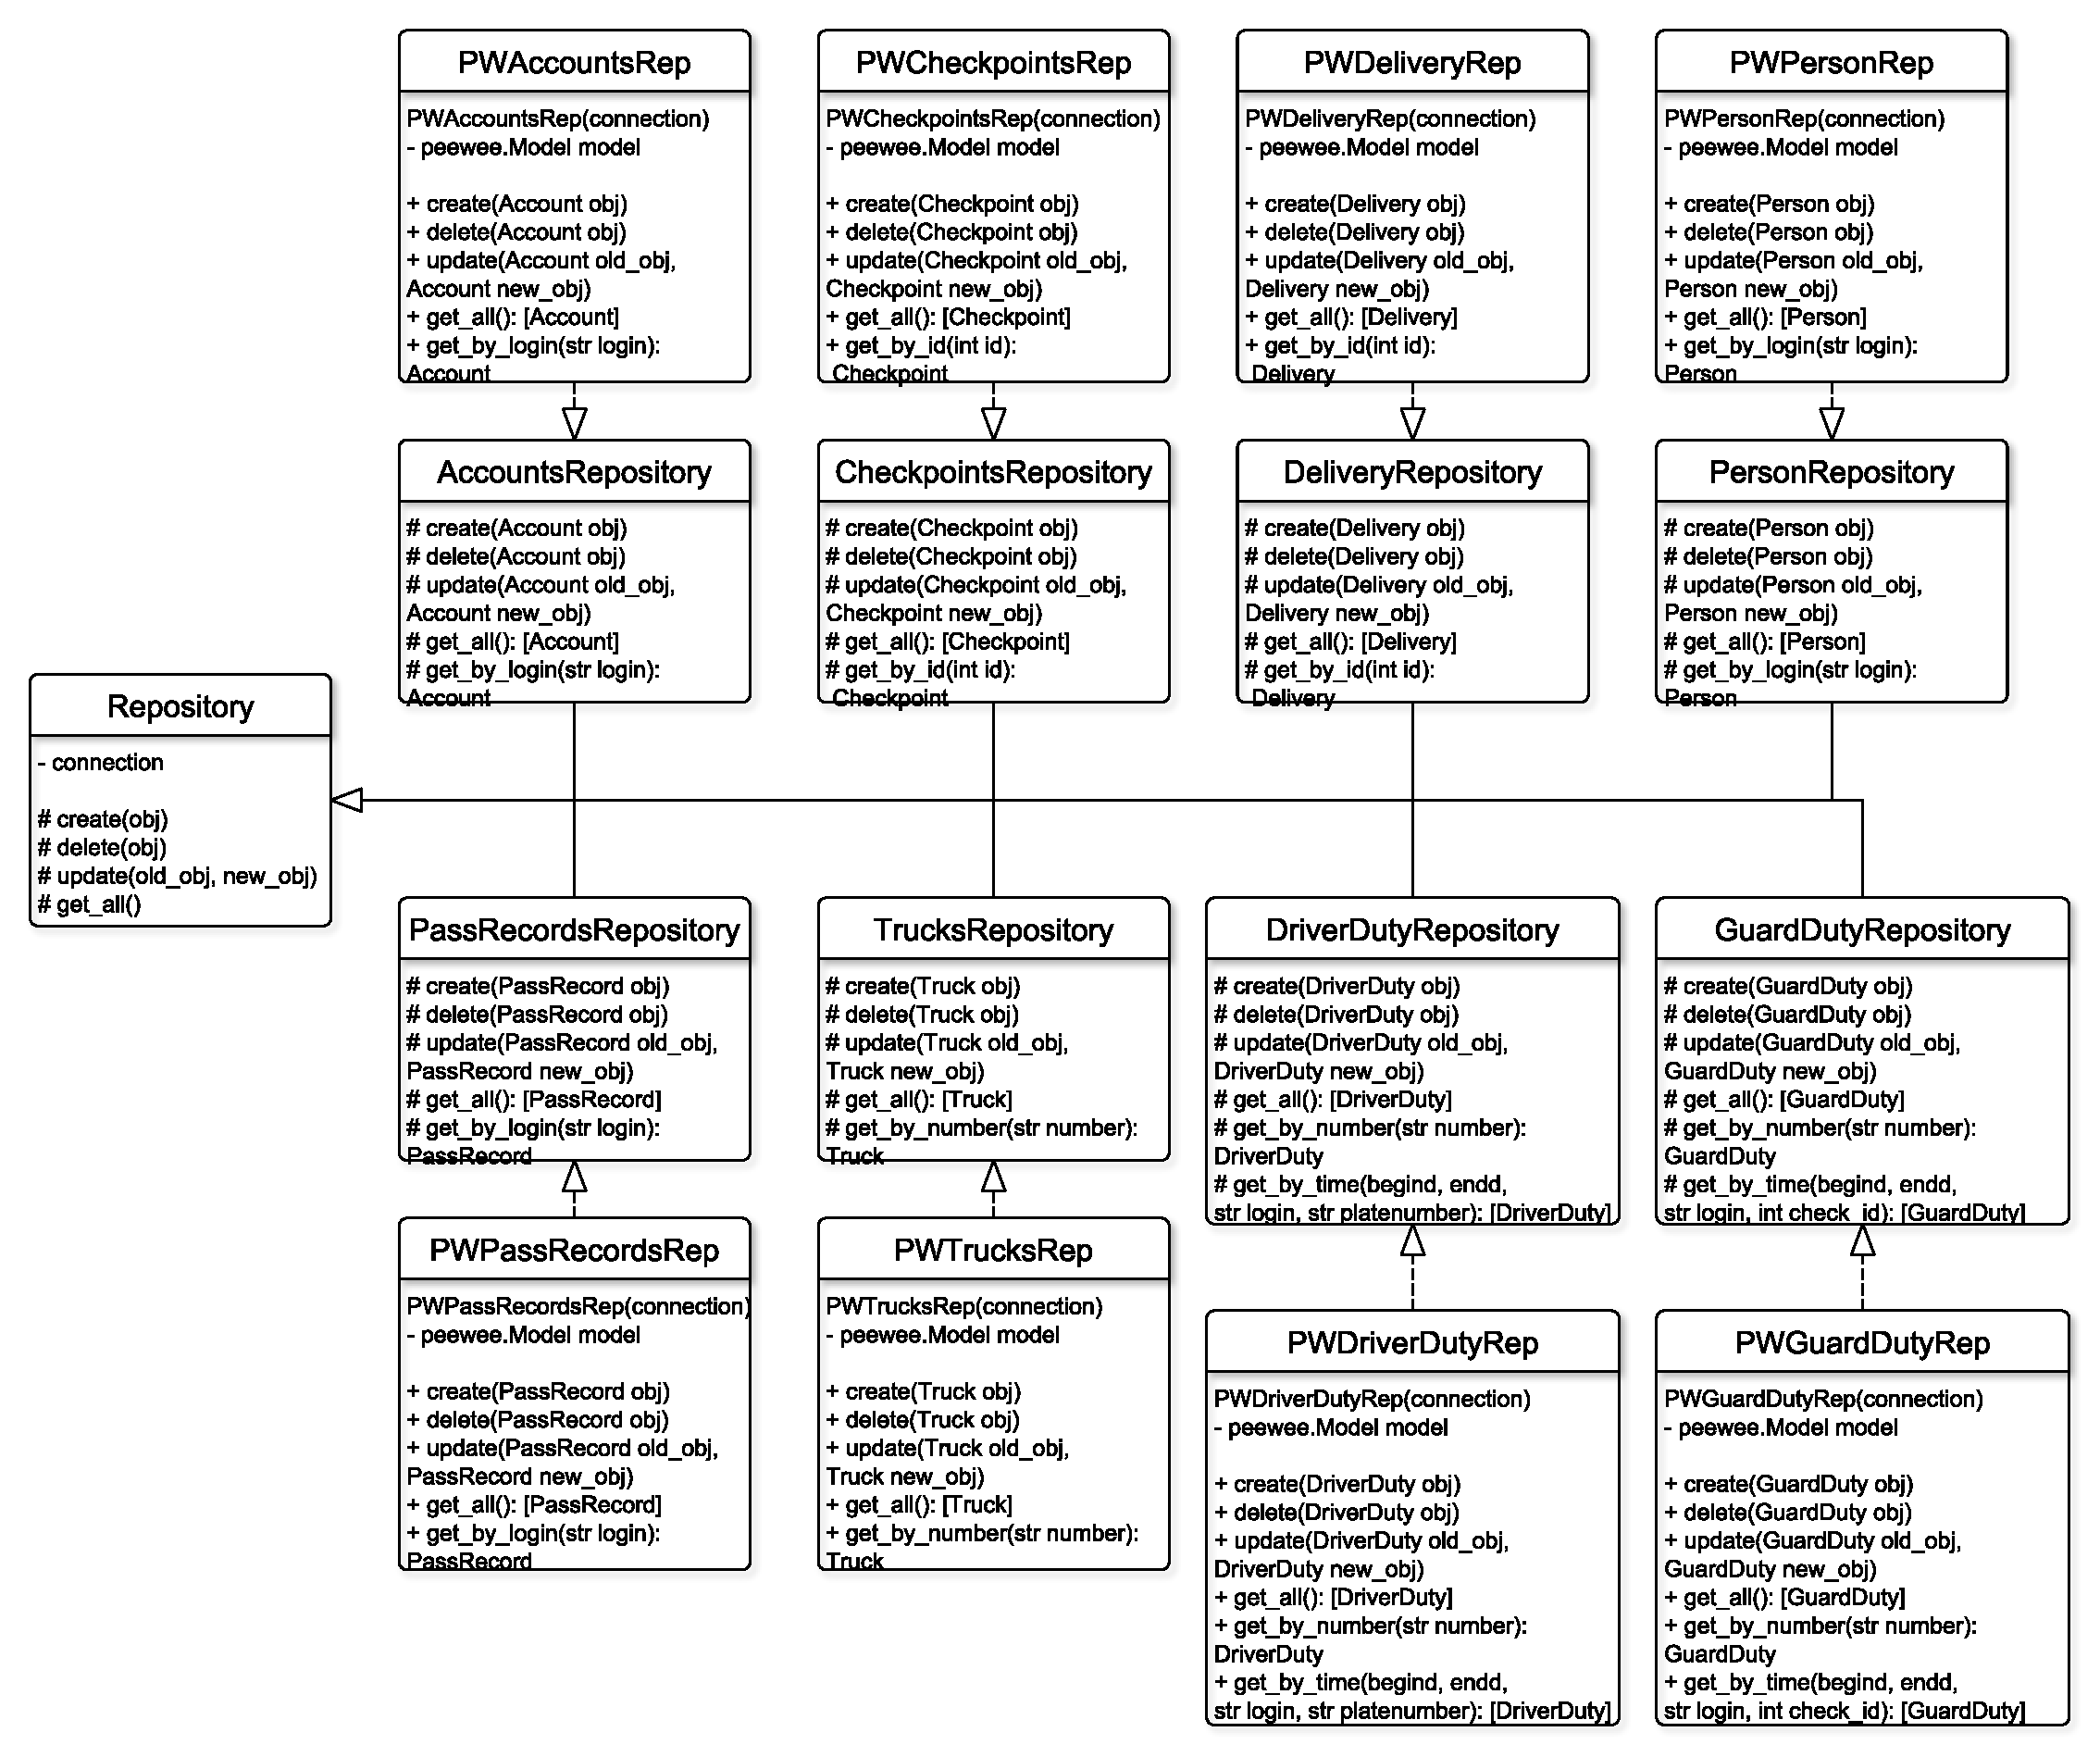
\includegraphics[height=14cm, width = 14cm]{uml/repsoitory.pdf}}
		{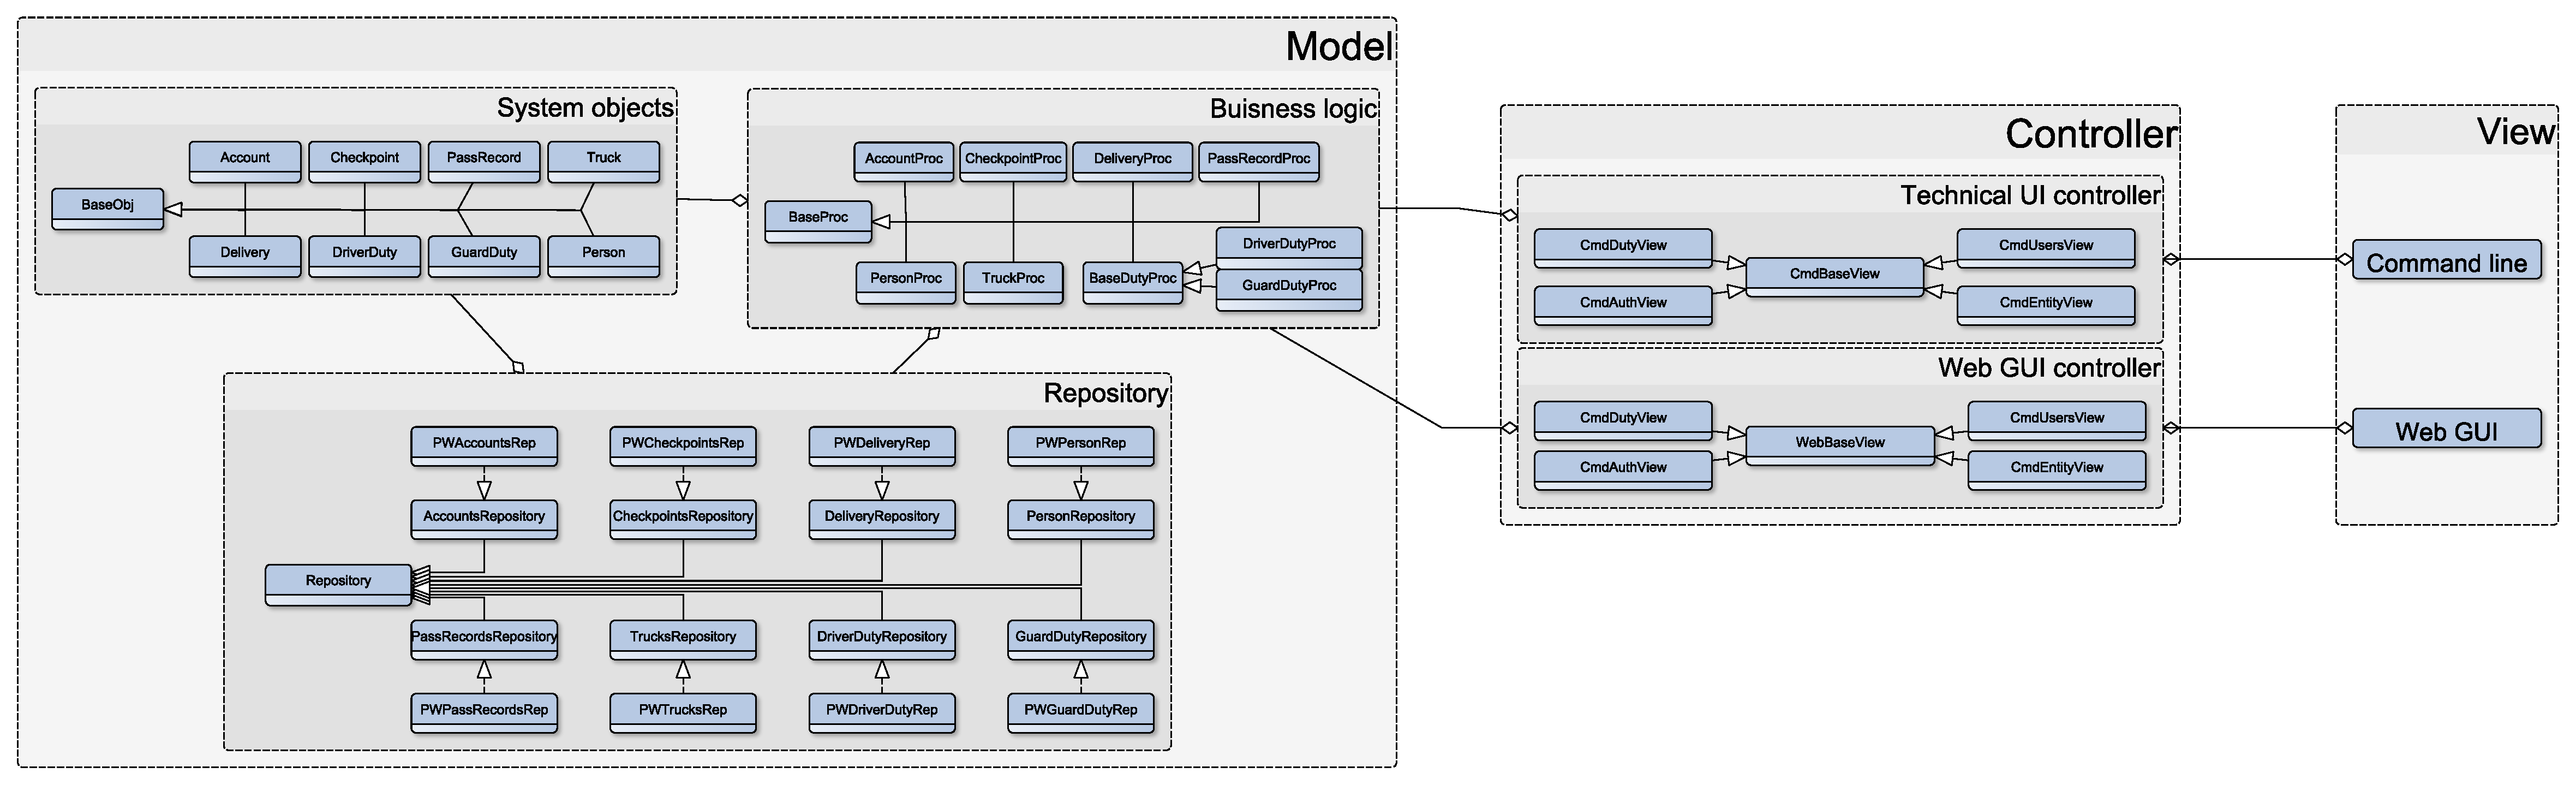
\includegraphics[scale=0.36, angle=-90]{uml/components.pdf}}
		\caption{UML-диаграмма компонента web-представления}
		\label{alluml_pic}
	\end{center}
\end{figure}

\section{Реализация базы данных}
\subsection{Создание таблиц}
В соответствии с ранее спроектированной моделью базы данных, были созданы 10 таблиц. Для примера в листинге \ref{lst:create_duty} приведён код генерации таблиц, связанных с дежурствами: DutyRules, GuardDuty и DriverDuty.

\begin{lstlisting}[caption = {Создание таблиц дежурств}, label=lst:create_duty]
CREATE TABLE IF NOT EXISTS DutyRules (
	RuleID		SERIAL		PRIMARY KEY,
	BeginDate	DATE		NOT NULL,
	EndDate		DATE,
	BeginTime	TIME		NOT NULL,
	EndTime		TIME		NOT NULL,
	DOW			VARCHAR(7)	NOT NULL
);
ALTER TABLE DutyRules ADD CONSTRAINT check_duty_dates
CHECK (BeginDate <= EndDate);
ALTER TABLE DutyRules ADD CONSTRAINT check_duty_times
CHECK (BeginTime < EndTime);
ALTER TABLE DutyRules ADD CONSTRAINT check_dow
CHECK (DOW SIMILAR TO '[0|1|2|3|4|5|6]{1,7}');

CREATE TABLE IF NOT EXISTS GuardDuty (
	DutyID 		 SERIAL	PRIMARY KEY,
	CheckpointID INT	REFERENCES Checkpoints(CheckpointID) NOT NULL,
	Login		 TEXT	REFERENCES Person(Login) NOT NULL,
	RuleID		 INT	REFERENCES DutyRules(RuleID) NOT NULL
);

CREATE TABLE IF NOT EXISTS DriverDuty (
	DutyID 		SERIAL	PRIMARY KEY,
	PlateNumber	TEXT	REFERENCES Trucks(PlateNumber) NOT NULL,
	Login		TEXT	REFERENCES Person(Login) NOT NULL,
	RuleID		INT		REFERENCES DutyRules(RuleID) NOT NULL
);
\end{lstlisting}

В таблице DutyRules в качестве первичного ключа (сокр. ПК) указан атрибут RuleID. Созданы ограничения в значениях дат начала и завершения расписания дежурства и времени начала и завершения смены. Также реализованно ограничение содержимого атрибута DOW: в данной строке могут храниться только цифры от 0 до 6, соответствующие дням недели, в количестве от одной до семи.

В таблицах GuardDuty и DriverDuty в качестве ПК выступает атрибут DutyID. Таже общим для двух таблиц является наличие внешних ключей Login и RuleID, ссылающихся на одноимённые поля в таблицах Person и DutyRules соотвественно. Для GuardDuty также существует внешний ключ CheckpointID, ссылающийся на таблицу Checkpoints, для DriverDuty дополнительный внешний ключ это PlateNumber, связанный с таблицей Trucks. Все внешние ключи содержат ограничение NOT NULL, так как они являются обязательными в данных сущностях.

\subsection{Ролевая модель}
Для создания прав доступа выделенных ролей к различным данным была реализована ролевая модель на уровне базы данных. Выделено следующие четыре роли:
\begin{itemize}
	\item admin - роль администратора;
	\item guard - роль охранника;
	\item driver - роль водителя;
	\item unverif - роль неподтверждённого сотрудника.
\end{itemize}

Код создания описанных ролей приведён в листингах \ref{lst:admin_role}--\ref{lst:unverif_role}

\begin{lstlisting}[caption = {Релизация роли admin}, label=lst:admin_role]
CREATE ROLE admin WITH
	LOGIN
	SUPERUSER
	PASSWORD 'admin';
\end{lstlisting}

\begin{lstlisting}[caption = {Релизация роли guard}, label=lst:guard_role]
CREATE ROLE guard WITH
	LOGIN
	PASSWORD 'guard';

GRANT SELECT, INSERT ON Passrecords TO guard;
GRANT SELECT ON Accounts TO guard;
GRANT SELECT ON Person TO guard;
GRANT SELECT ON GuardDutys TO guard;
GRANT SELECT, INSERT ON PassRecords TO guard;
GRANT ALL PRIVILEGES ON SEQUENCE passrecords_recordid_seq TO guard;
GRANT SELECT ON Checkpoints TO guard;
GRANT SELECT ON Trucks TO guard;
GRANT INSERT ON LogActions TO guard;

GRANT SELECT ON GuardDuty TO guard;
GRANT SELECT ON DutyRules TO guard;
\end{lstlisting}

\begin{lstlisting}[caption = {Релизация роли driver}, label=lst:driver_role]
CREATE ROLE driver WITH
	LOGIN
	PASSWORD 'driver';

GRANT SELECT, INSERT ON Passrecords TO driver;
GRANT SELECT ON Accounts TO driver;
GRANT SELECT ON Person TO driver;
GRANT SELECT, UPDATE ON Delivery TO driver;
GRANT SELECT ON DriverDutys TO driver;
GRANT INSERT ON LogActions TO driver;

GRANT SELECT ON DriverDuty TO driver;
GRANT SELECT ON DutyRules TO driver;
\end{lstlisting}

\begin{lstlisting}[caption = {Релизация роли unverif}, label=lst:unverif_role]
CREATE ROLE unverif WITH
	LOGIN
	PASSWORD 'unverif';

GRANT SELECT ON Accounts TO unverif;
GRANT SELECT ON Person TO unverif;
GRANT INSERT ON LogActions TO unverif;
\end{lstlisting}


\subsection{Триггеры}
В базе данных реализованы триггеры соответствующие спроектированным схемам.

На листинге \ref{lst:pass_trig} приведена реализация триггера LogPassRecordIns, осуществляющего логирование информации добавления записи о проезде.
\begin{lstlisting}[caption = {Релизация триггера LogPassRecordIns}, label=lst:pass_trig]
CREATE OR REPLACE FUNCTION LogPassRecordIns()
RETURNS TRIGGER AS $$ BEGIN
	INSERT INTO LogActions VALUES 
		(current_user, NOW(), 'Created pass record №' || NEW.RecordID);
	RETURN NULL;
END; $$ LANGUAGE plpgsql;

CREATE TRIGGER LogPassRecordIns BEFORE INSERT
ON PassRecords FOR EACH ROW
	EXECUTE PROCEDURE LogPassRecordIns();
\end{lstlisting}

На листинге \ref{lst:deli_trig} приведена реализация триггера LogDeliveryUpd, осуществляющего логирование информации о добавлении заказа.
\begin{lstlisting}[caption = {Релизация триггера LogDeliveryUpd}, label=lst:deli_trig]
CREATE OR REPLACE FUNCTION LogDeliveryUpd()
RETURNS TRIGGER AS $$ BEGIN
	IF NEW.Status = 'delivered' THEN 
		INSERT INTO LogActions VALUES 
		(current_user, NOW(), 'Set delivery №' || NEW.OrderID || ' status = delivered');
	ELSE
		INSERT INTO LogActions VALUES 
		(current_user, NOW(), 'Assigned delivery №' || NEW.OrderID || ' to ' || NEW.Login);
	END IF;
RETURN NULL;
END; $$ LANGUAGE plpgsql;

CREATE TRIGGER LogDeliveryUpd BEFORE UPDATE
ON Delivery FOR EACH ROW
	EXECUTE PROCEDURE LogDeliveryUpd();
\end{lstlisting}

На листинге \ref{lst:acc_trig} приведена реализация триггера BanActiveAccDel, осуществляющего запрет удаления подтверждённых сотрудников.
\begin{lstlisting}[caption = {Релизация триггера BanActiveAccDel}, label=lst:acc_trig]
CREATE OR REPLACE FUNCTION BanActiveAccDel()
RETURNS TRIGGER AS $$ BEGIN
	IF (current_user = 'admin') AND (OLD.PersType NOT LIKE '~%') 
	THEN
		RAISE EXCEPTION 'cannot delete active user';
	END IF;
	RETURN OLD;
END; $$ LANGUAGE plpgsql;

CREATE TRIGGER BanActiveAccDel BEFORE DELETE
ON Accounts FOR EACH ROW
	EXECUTE PROCEDURE BanActiveAccDel();
\end{lstlisting}

\subsection{Функции}
В работе программы особую сложность представляет работа с расписаниями дежурств, а также с самими дежурствами водителей. Пояснение реализованных функций для каждой таблицы приведено дальше. Все листинге расположены в приложении А, стр. \pageref{attachmentA}.
\begin{itemize}
	\item Таблица DutyRules. Требуется осуществлять выборку дежурств в определённом диапазоне дат, нахождение активных дежурств в определённый момент времени, в том числе и в текущий. Код функций приведён в листинге \ref{lst:duty_rules_f}.
	\item Таблицы DriverRules и GuardRules. Для дежурств требуется осуществлять поиск по логину и номеру КПП в случае охранника или номеру машины в случае водителя. Также требуется учитывать диапазон дат, в котором осуществляется поиск или определённый момент времени. Код описанных функций приведён в листингах \ref{lst:driver_duty_f} и \ref{lst:guard_duty_f} для таблиц DriverRules и GuardRules соотвественно.
\end{itemize}

\newpage
\section{Интерфейс приложения}
Для авторизованного пользователя в заголовке каждой страницы содержится панель навигации, предоставляющая возможность перейти на все страницы, функционально соответствующие его роли. Данная панель изображена на примере администратора на рисунке \ref{sc:navbar}. Некоторые пункты меню являются выпадающими, их можно открыть наведением мыши. Также в левом углу панели присутствует элемент информационного или ошибочного сообщения.

На рисунке \ref{sc:navbar} изображена страница профиля сотрудника, на котором он может посмотреть всю свою личную информацию. Просматривать свою страницу может пользователь с любой ролью. Для водителя на странице профиля также отображается история его заказов (на рисунке \ref{sc:driver_profile}).

\begin{figure}[h!] 
	\begin{center}
		%		{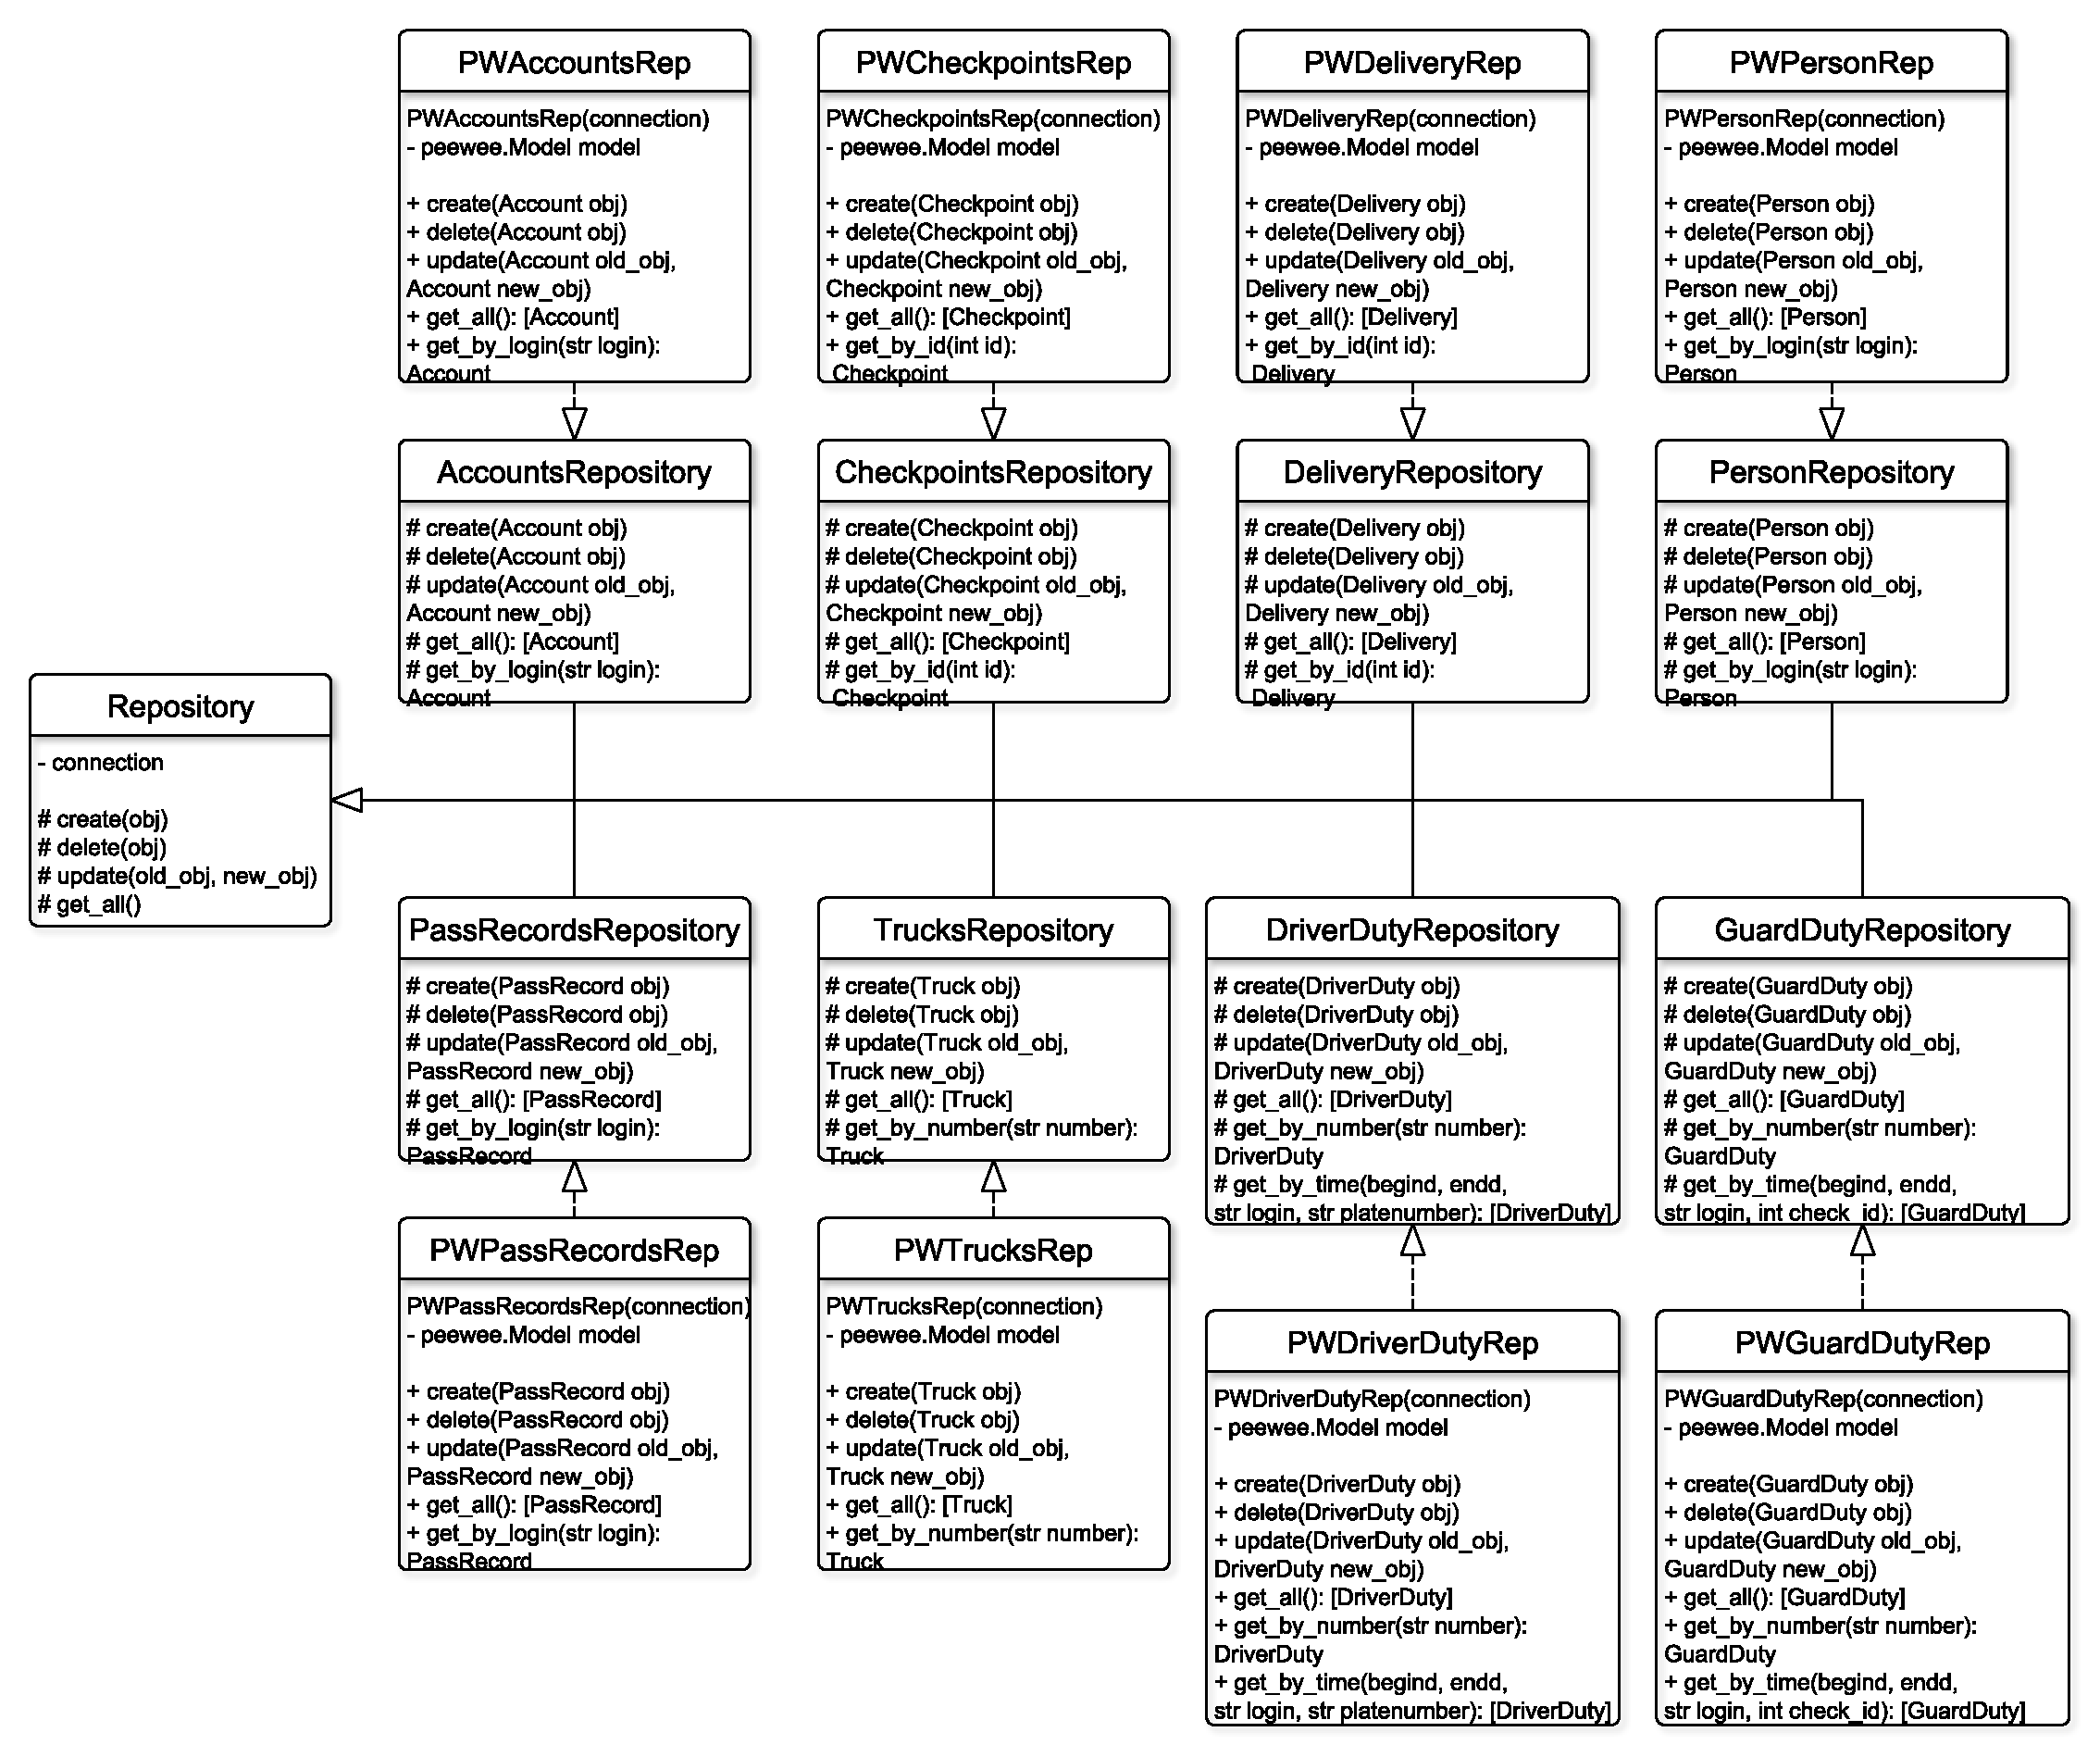
\includegraphics[height=14cm, width = 14cm]{uml/repsoitory.pdf}}
		{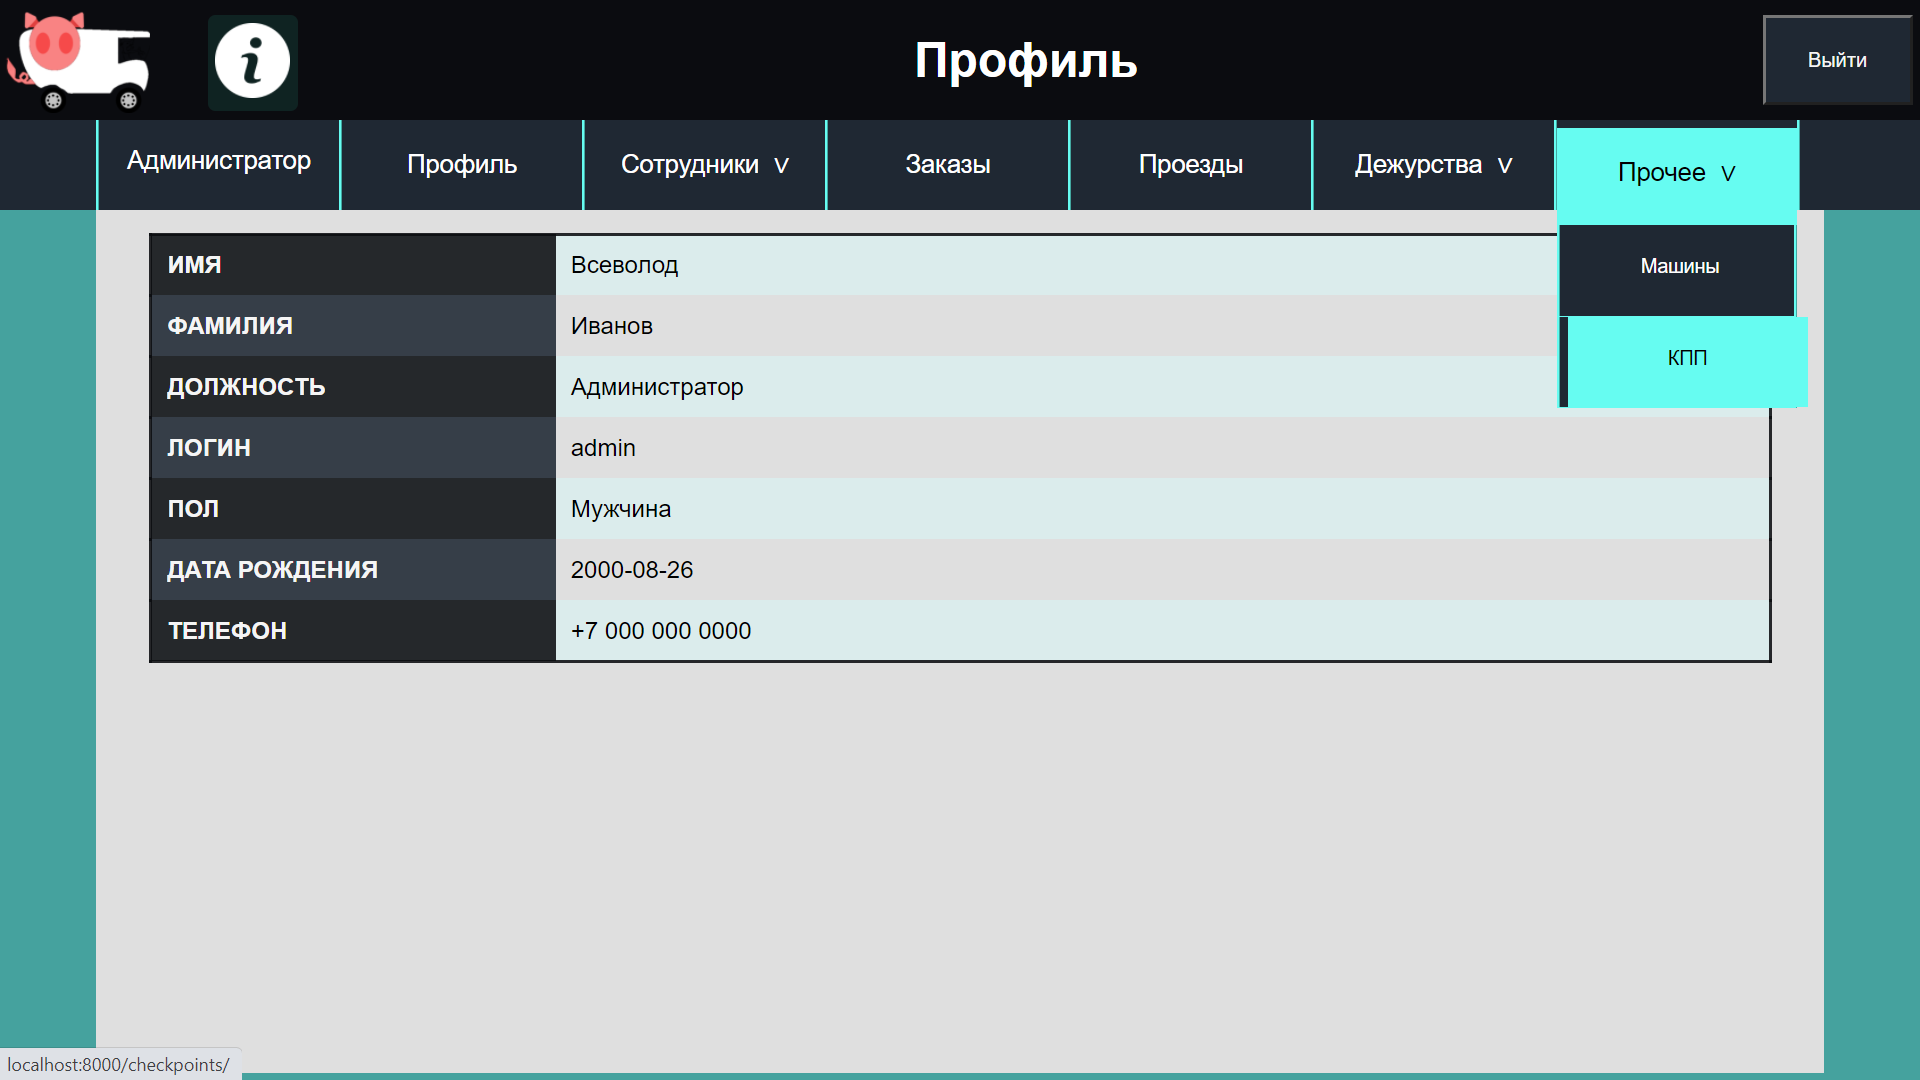
\includegraphics[scale=0.45, angle=0]{sc/admin_profile}}
		\caption{Страница профиля администратора}
		\label{sc:navbar}
	\end{center}
\end{figure}

\begin{figure}[h!] 
	\begin{center}
		%		{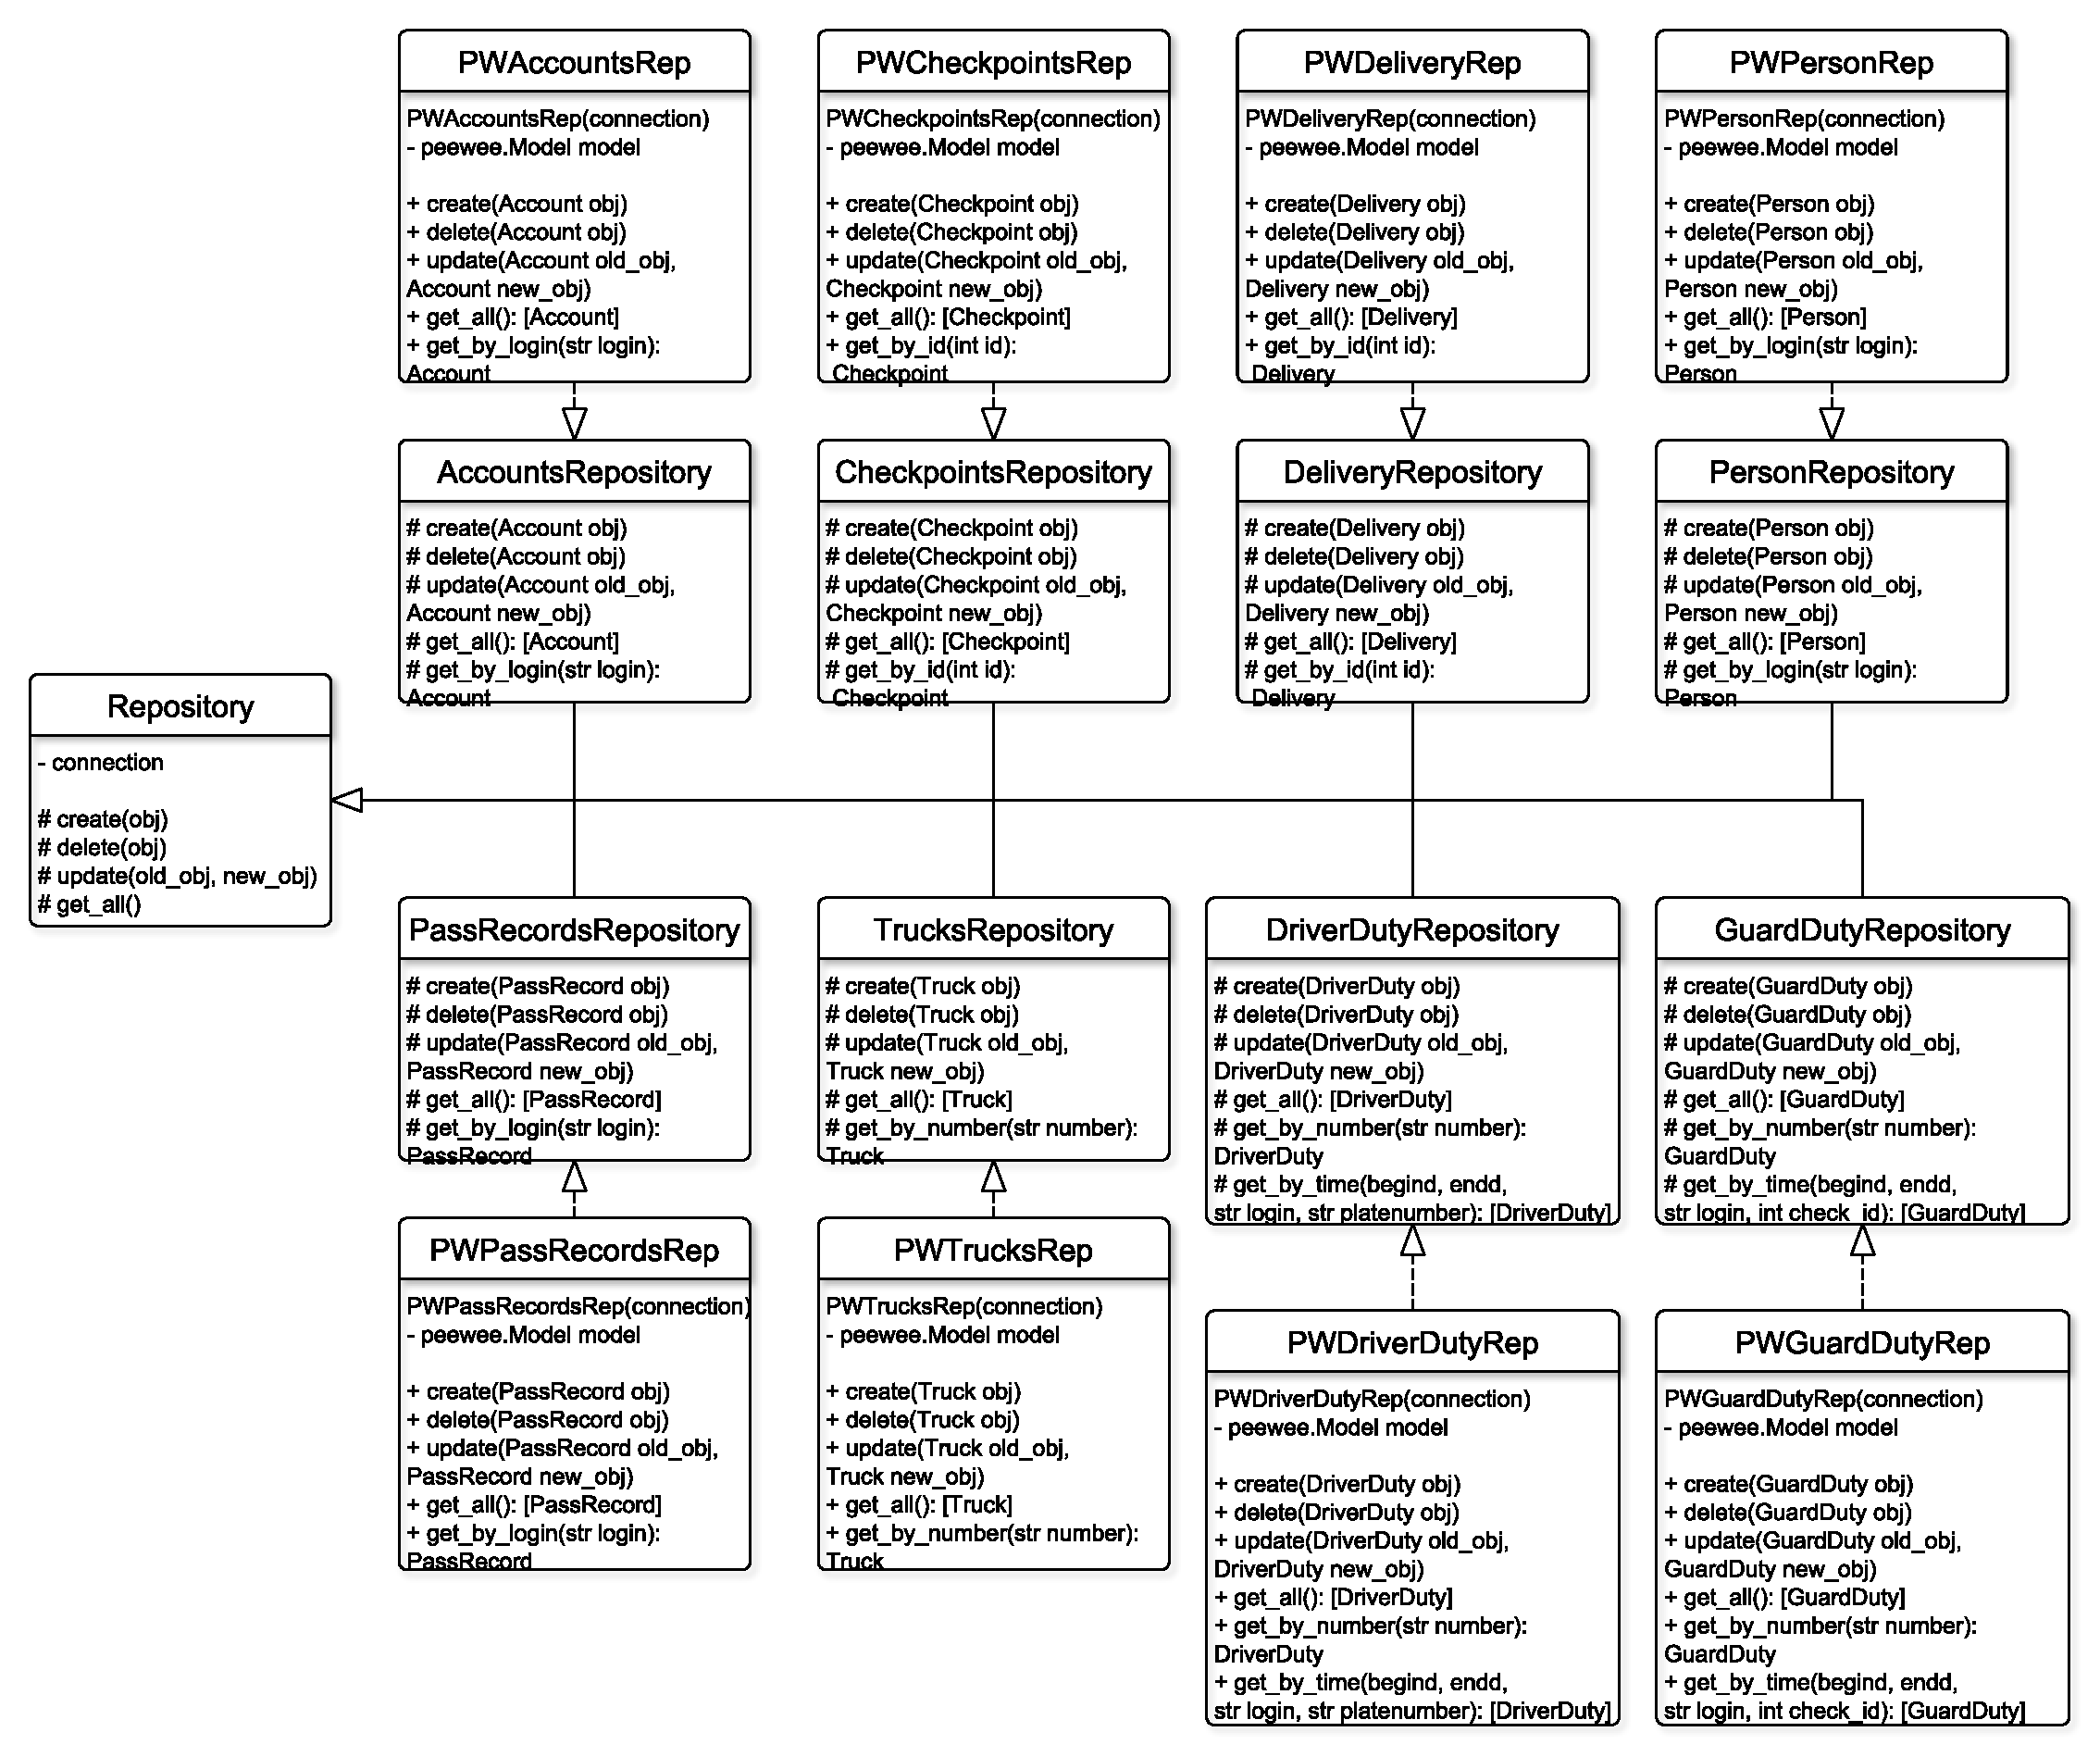
\includegraphics[height=14cm, width = 14cm]{uml/repsoitory.pdf}}
		{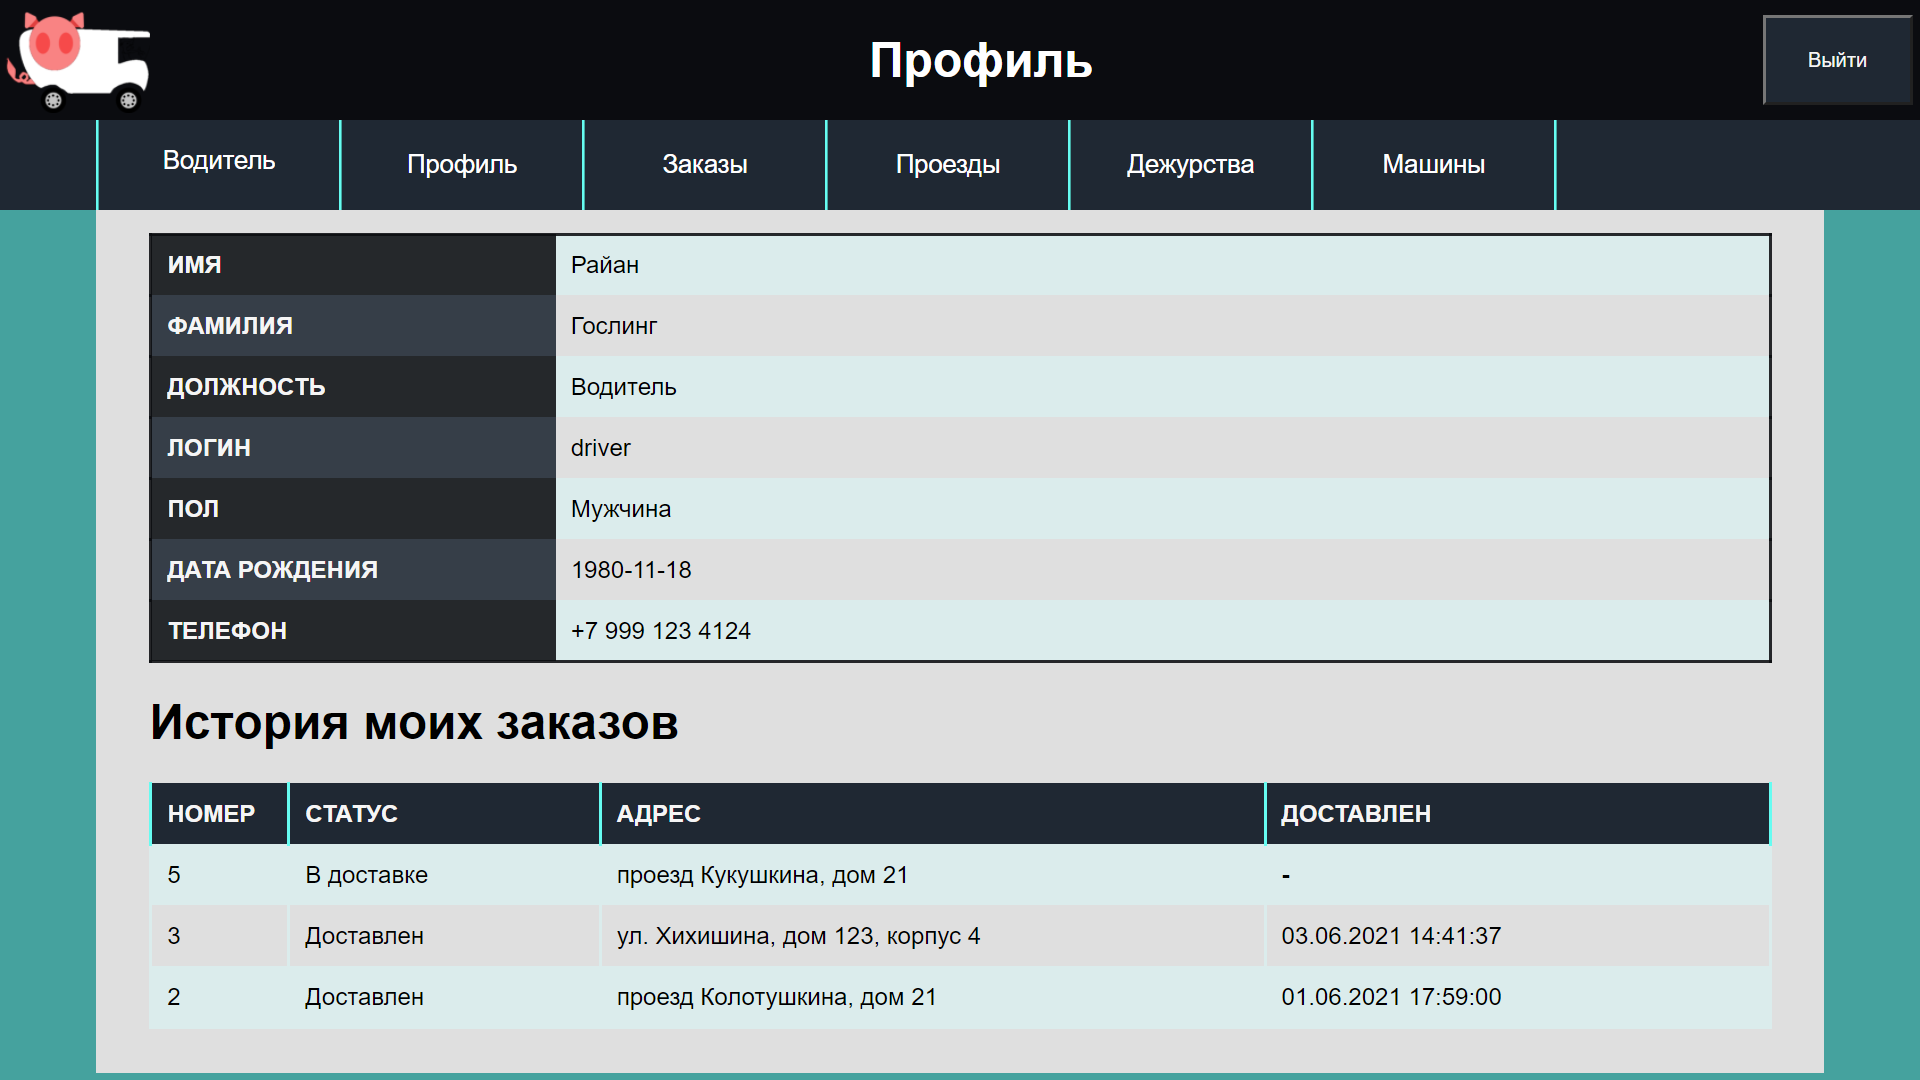
\includegraphics[scale=0.45, angle=0]{sc/driver_profile}}
		\caption{История заказов (для профиля водителя)}
		\label{sc:driver_profile}
	\end{center}
\end{figure}

На рисунке \ref{sc:all_profiles} представлена страница просмотра всех сотрудников. С помощью клика на ряд таблицы можно перейти на страницу конкретного сотрудника, описанная выше. Данный функционал доступен только для администратора.
\begin{figure}[h!] 
	\begin{center}
		%		{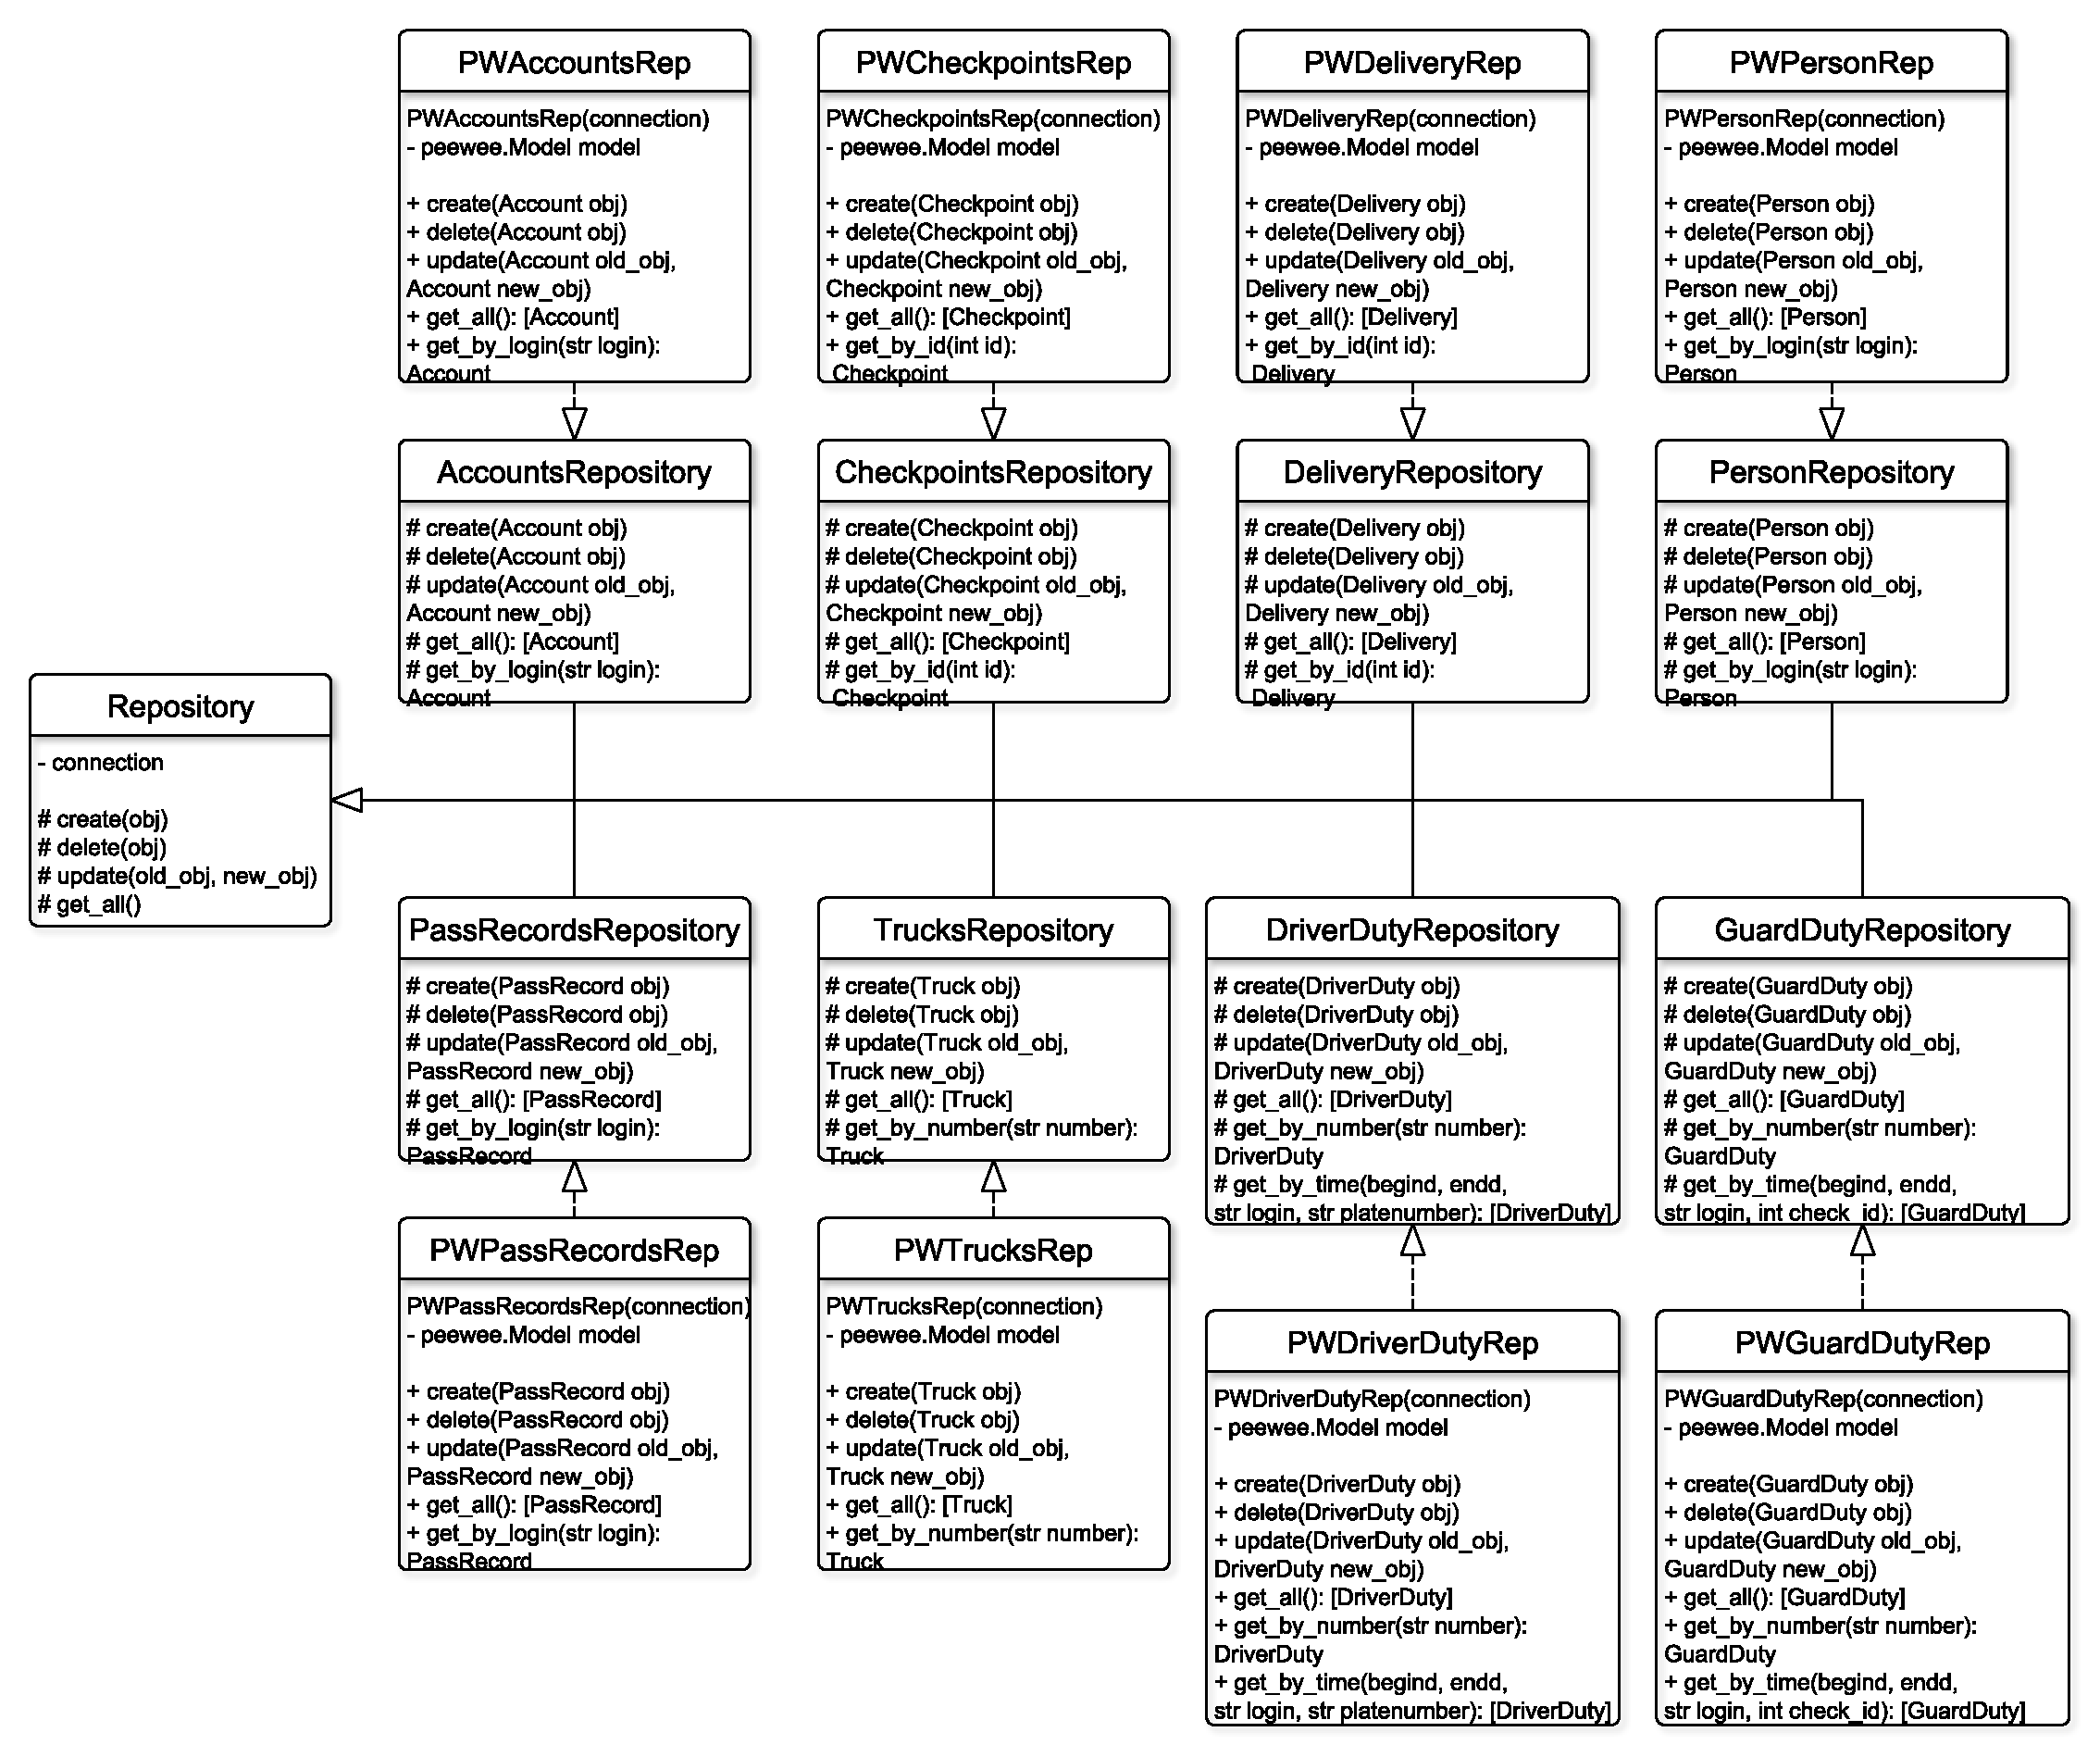
\includegraphics[height=14cm, width = 14cm]{uml/repsoitory.pdf}}
		{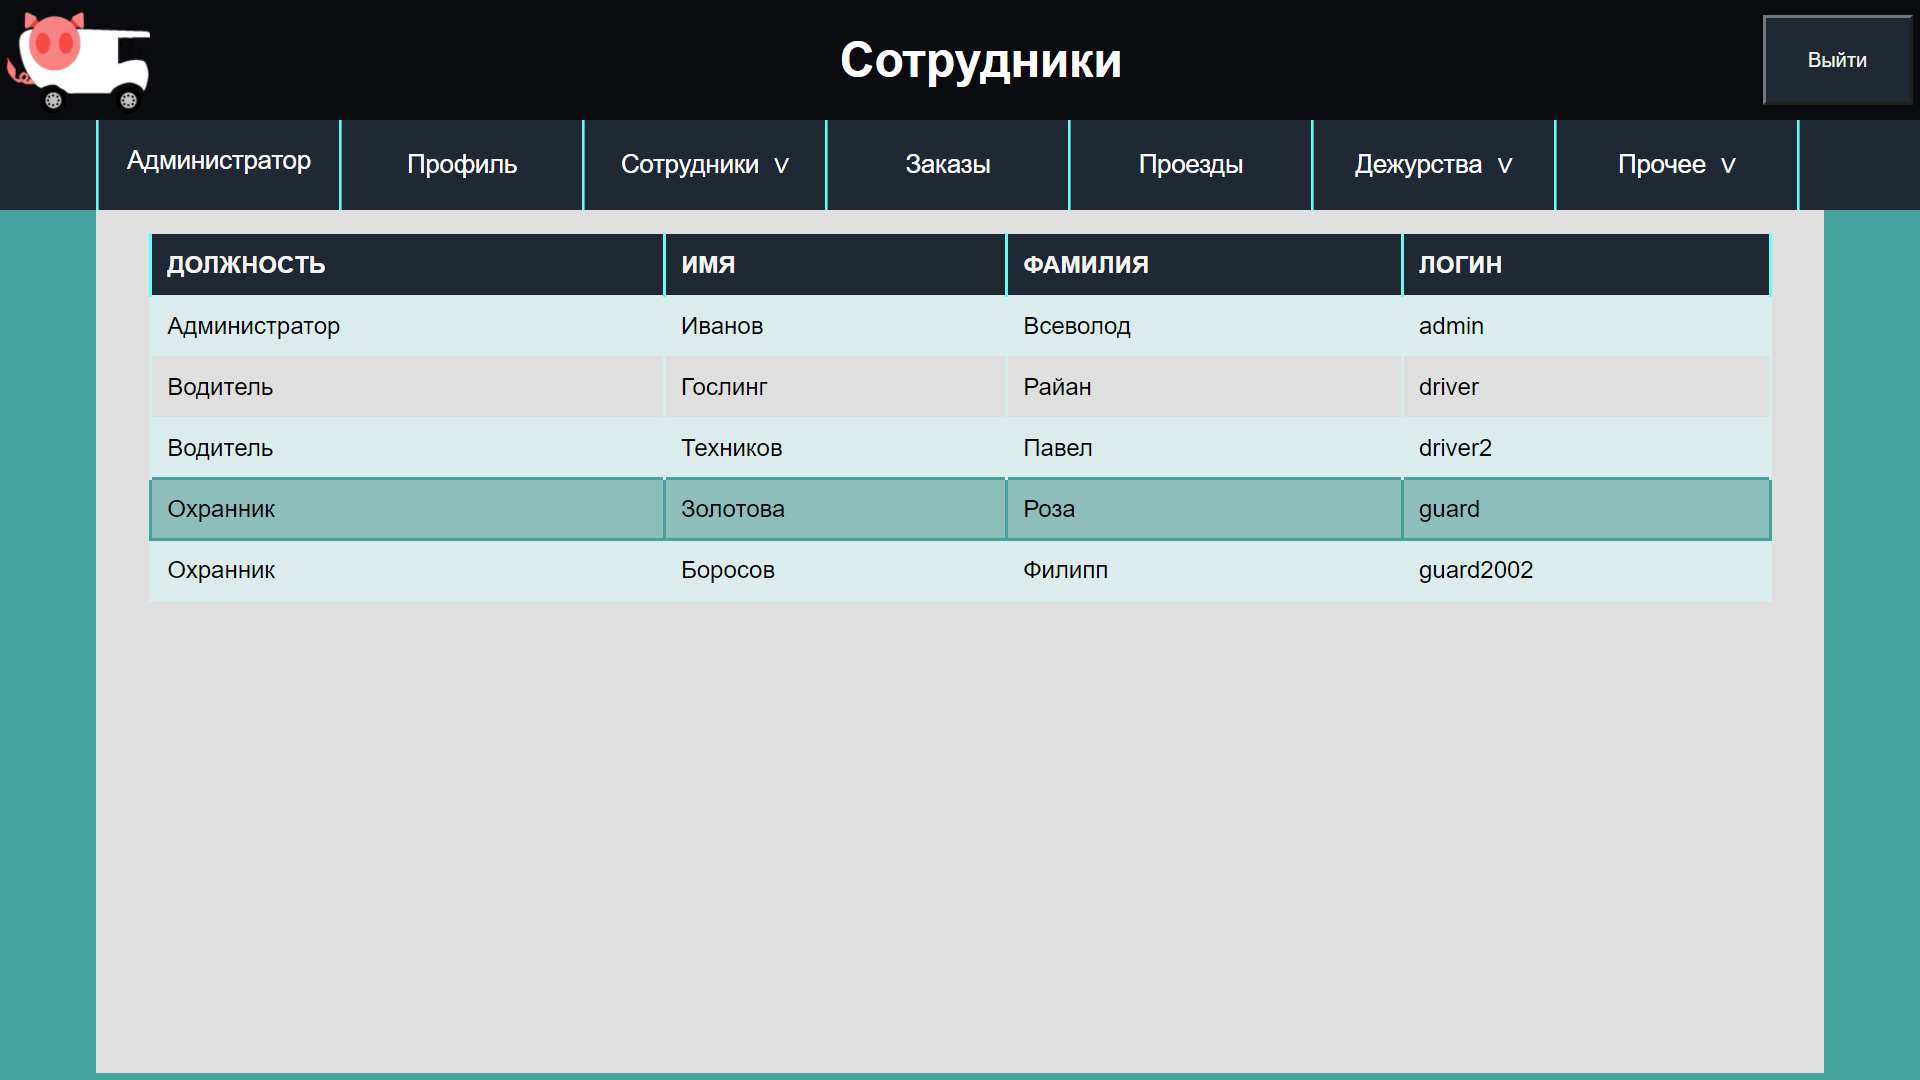
\includegraphics[scale=0.45, angle=0]{sc/all_profiles}}
		\caption{Страница просмотра всех сотрудников}
		\label{sc:all_profiles}
	\end{center}
\end{figure}

На рисунке \ref{sc:unver} представленна страница заявок на регистрацию. Заявки можно принять или отклонить кликом на соотв. кнопки. Данная страница также доступна только администратору. 
\begin{figure}[h!] 
	\begin{center}
		%		{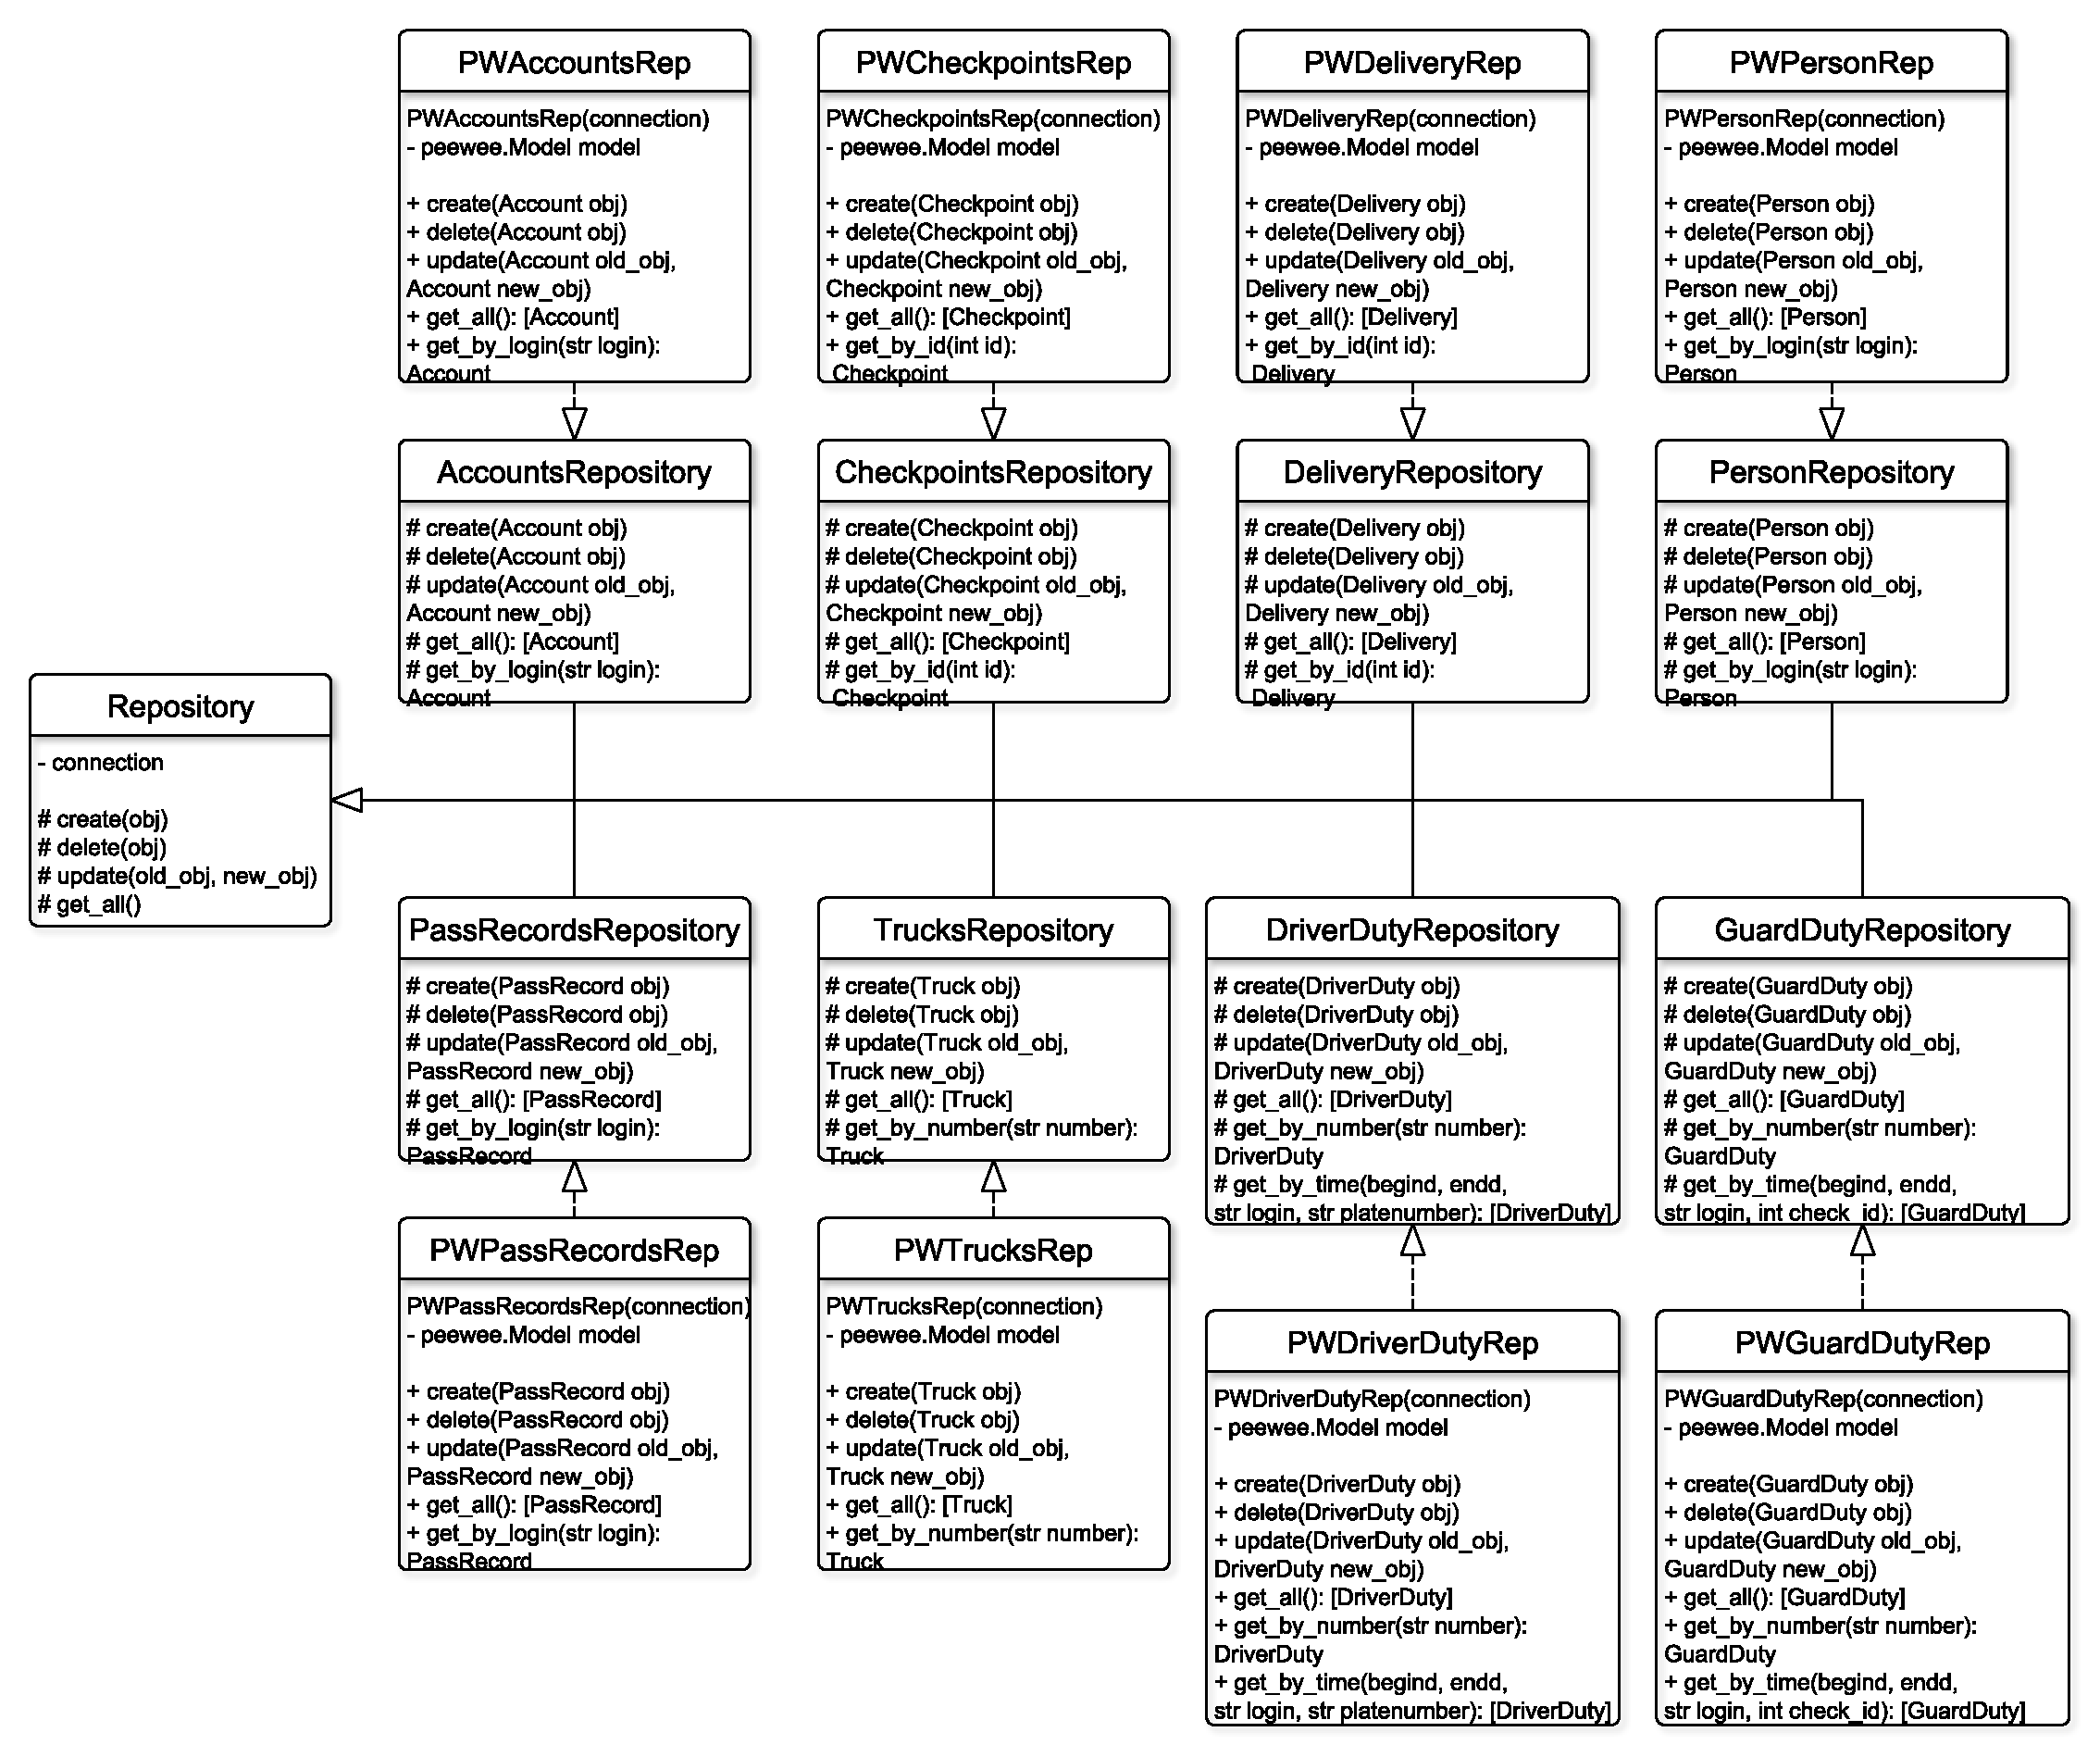
\includegraphics[height=14cm, width = 14cm]{uml/repsoitory.pdf}}
		{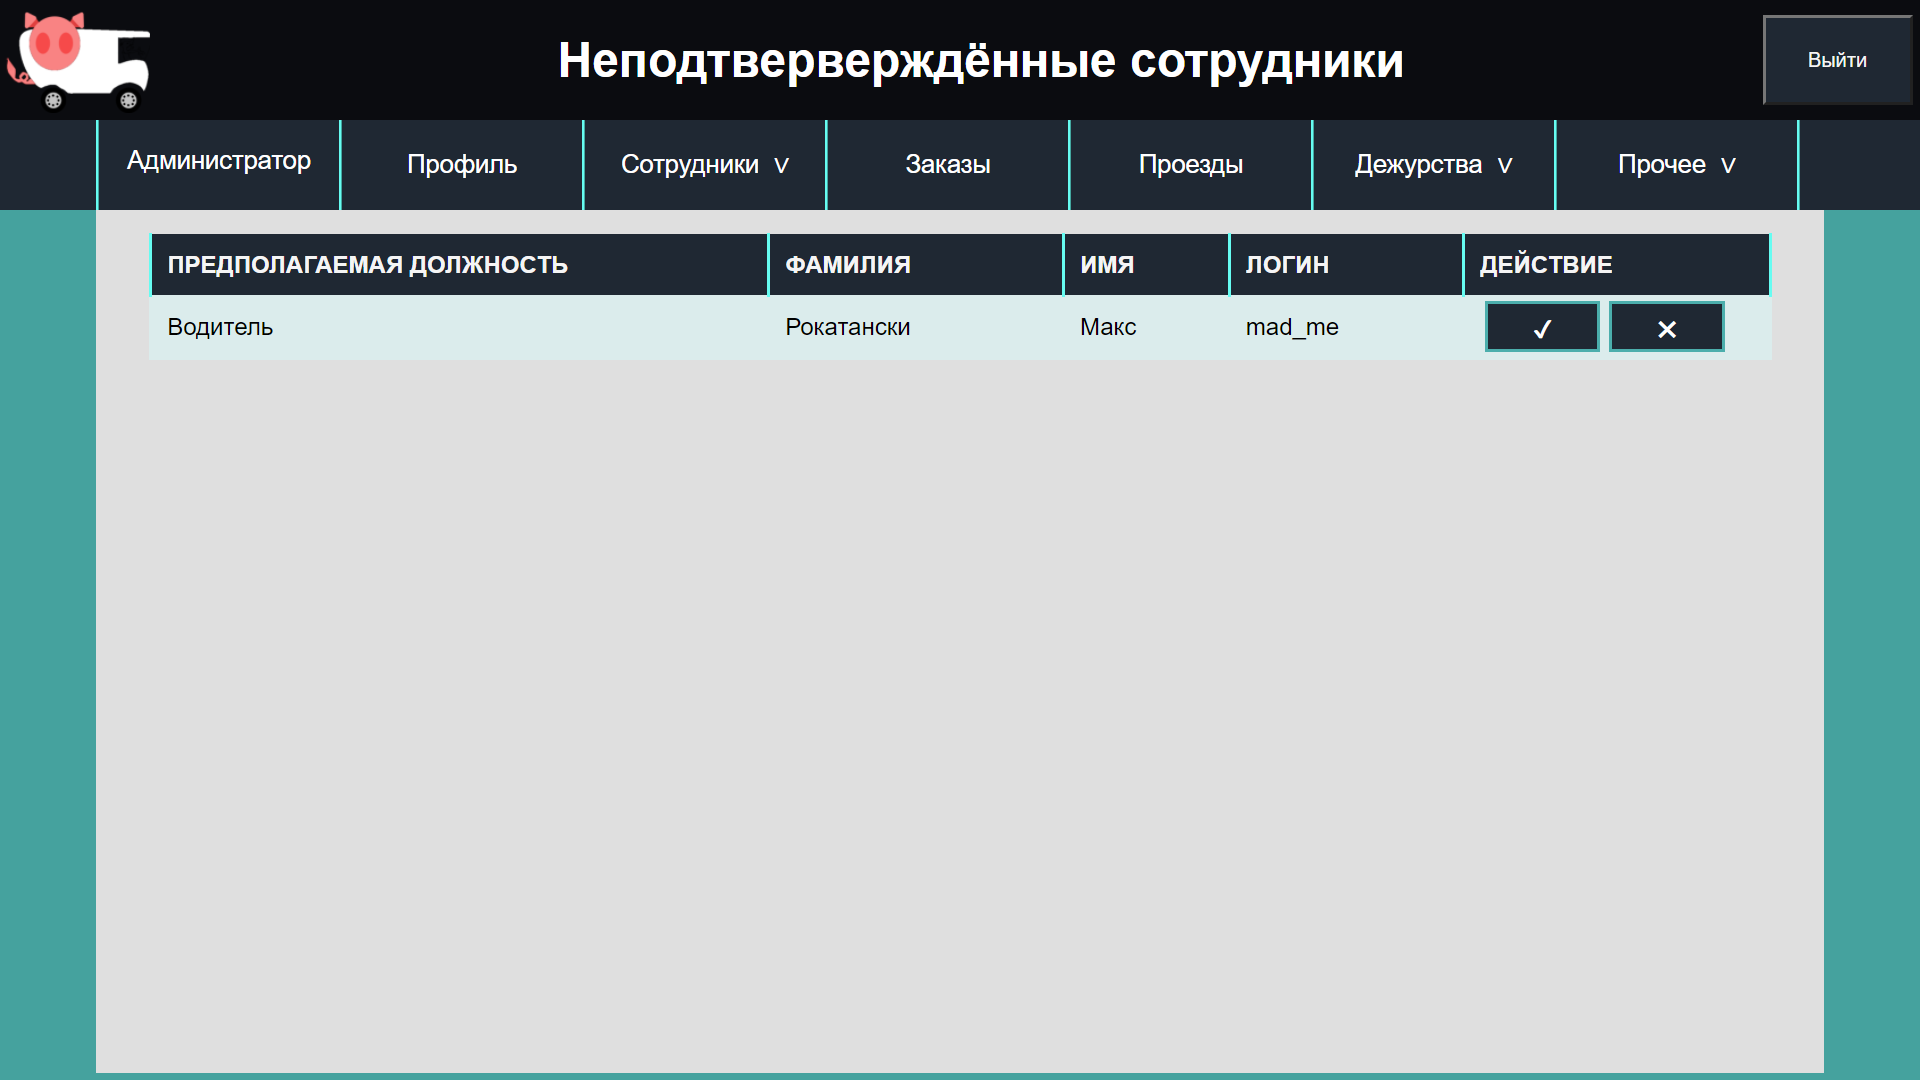
\includegraphics[scale=0.43, angle=0]{sc/unver}}
		\caption{Страница просмотра заявок регистрации}
		\label{sc:unver}
	\end{center}
\end{figure}

На рисунке \ref{sc:all_delivery} изображена страница просмотра всех заказов. По клику на строку заказа можно перейти на страницу подробной информации о заказе. Просмотр этой страницы доступен для водителей и администраторов. Для последних также существует возможность создать заказ в всплывающем окне.
\begin{figure}[h!] 
	\begin{center}
		%		{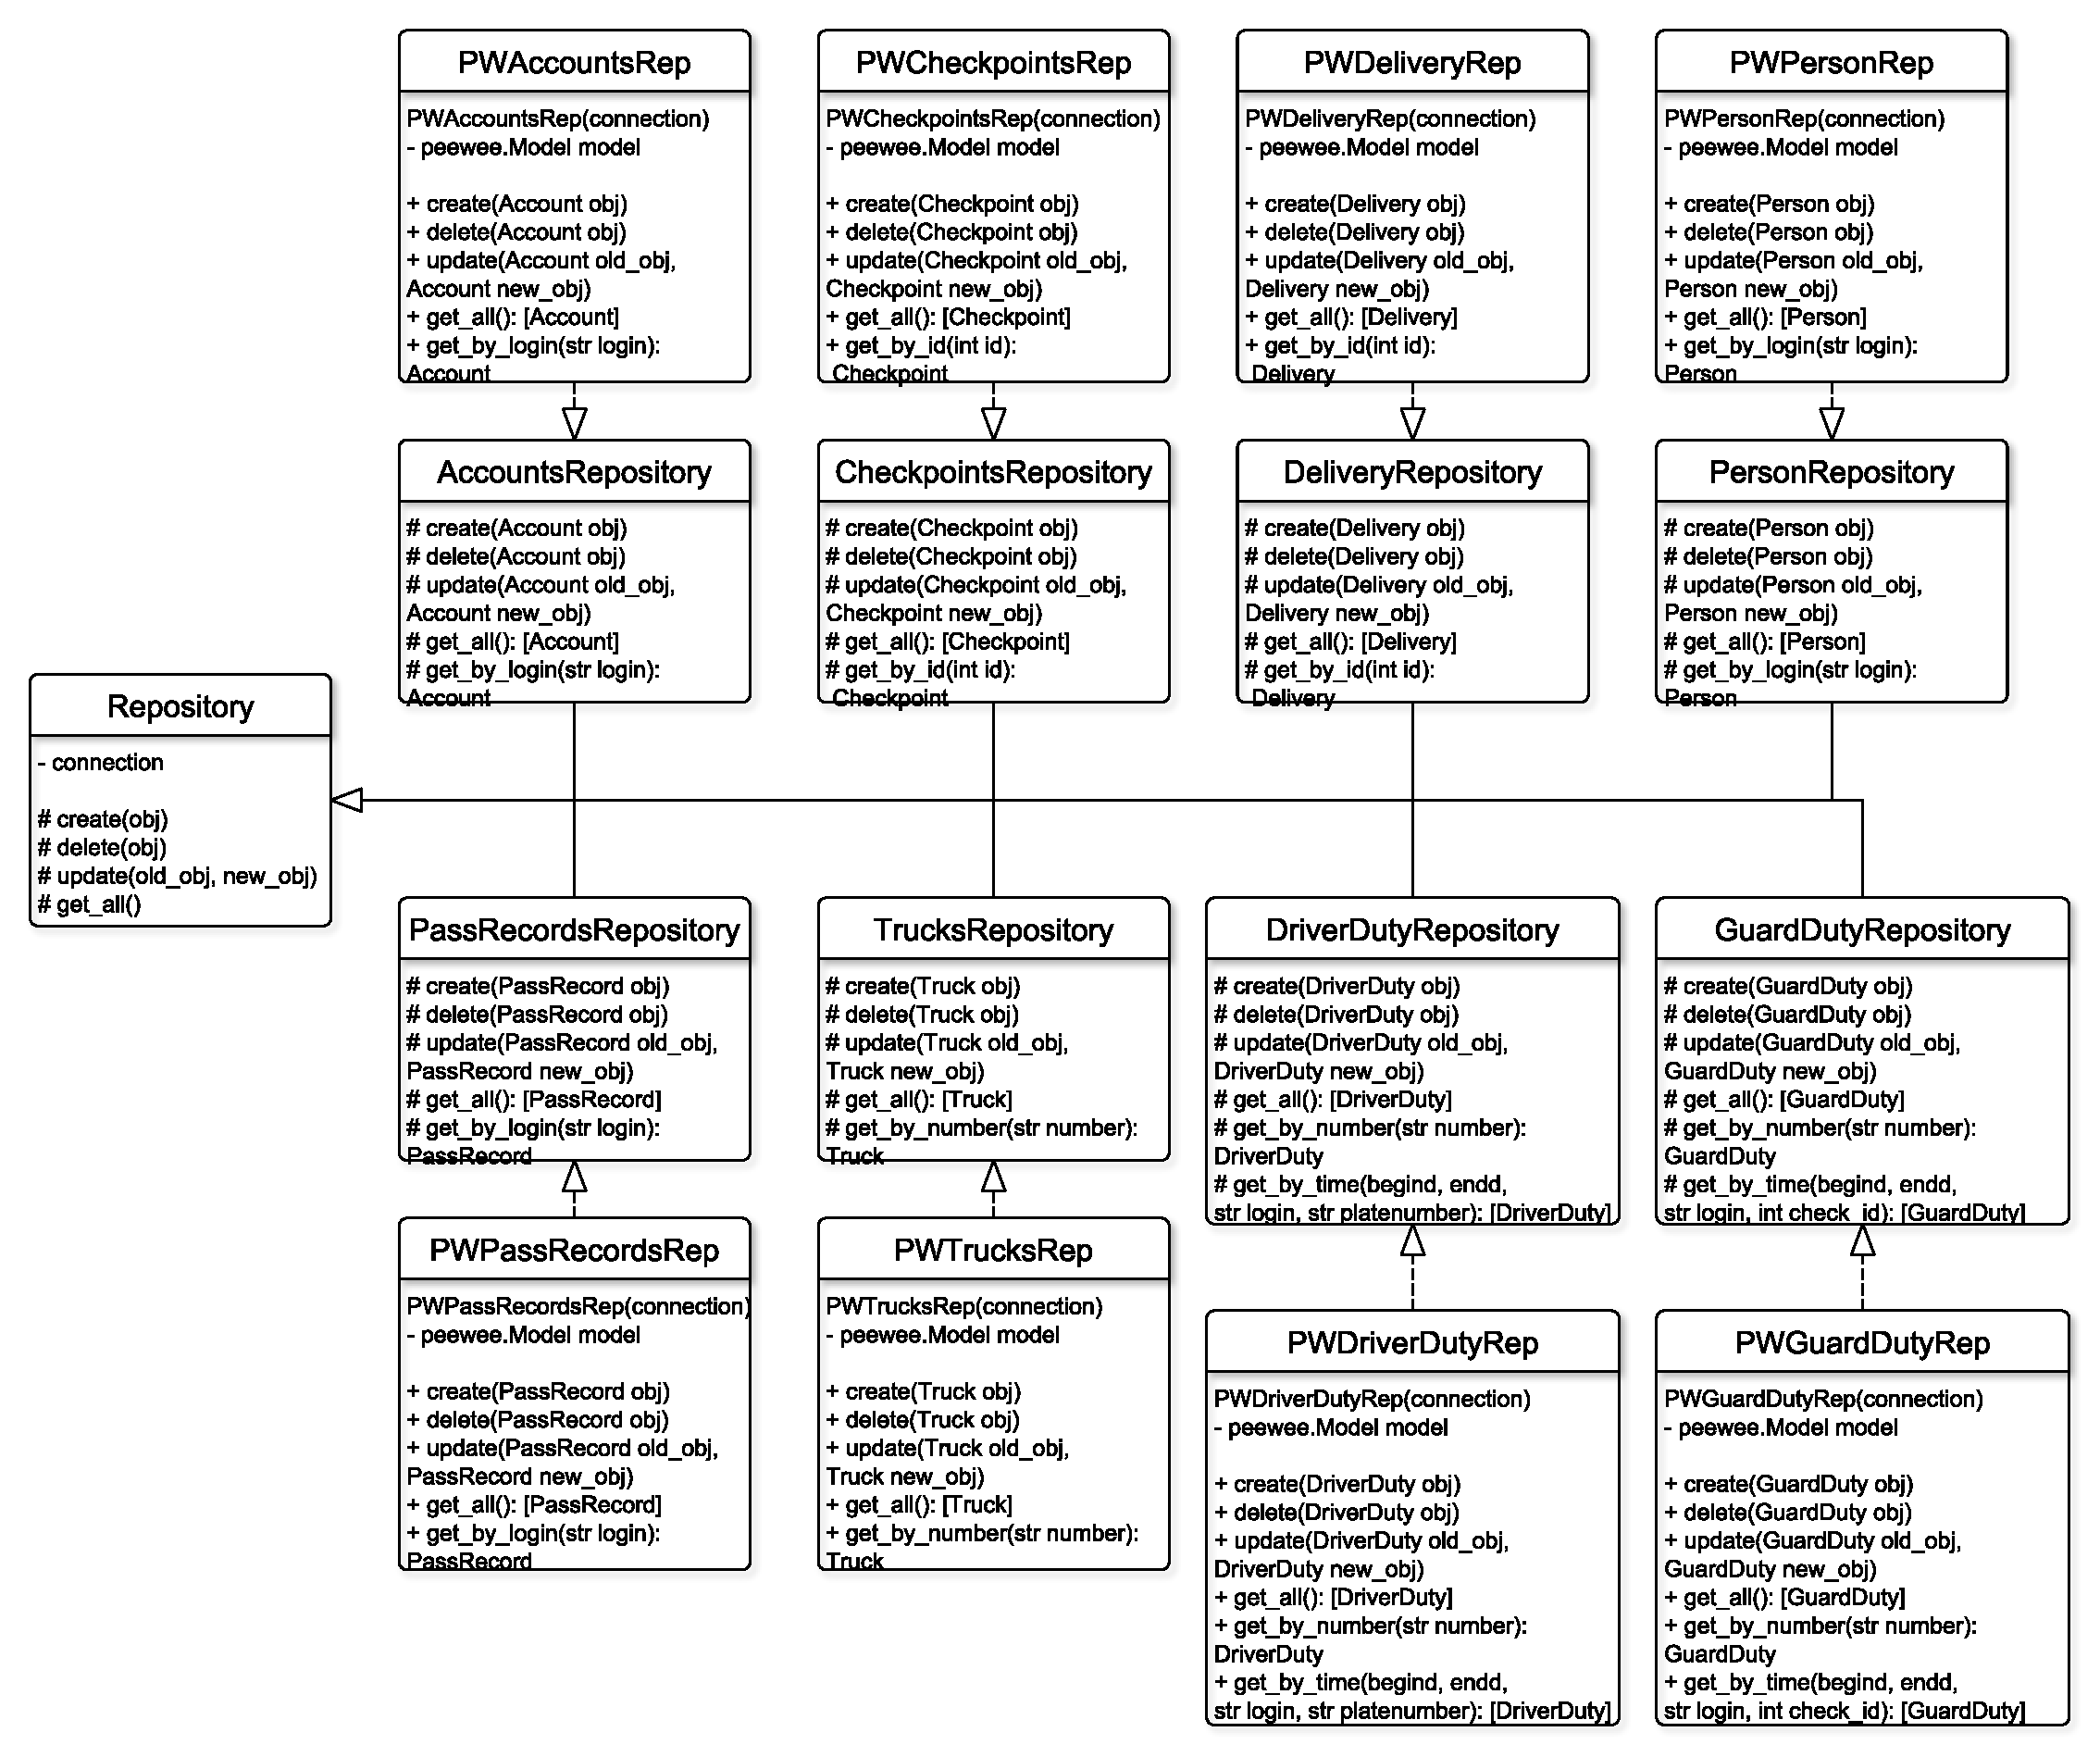
\includegraphics[height=14cm, width = 14cm]{uml/repsoitory.pdf}}
		{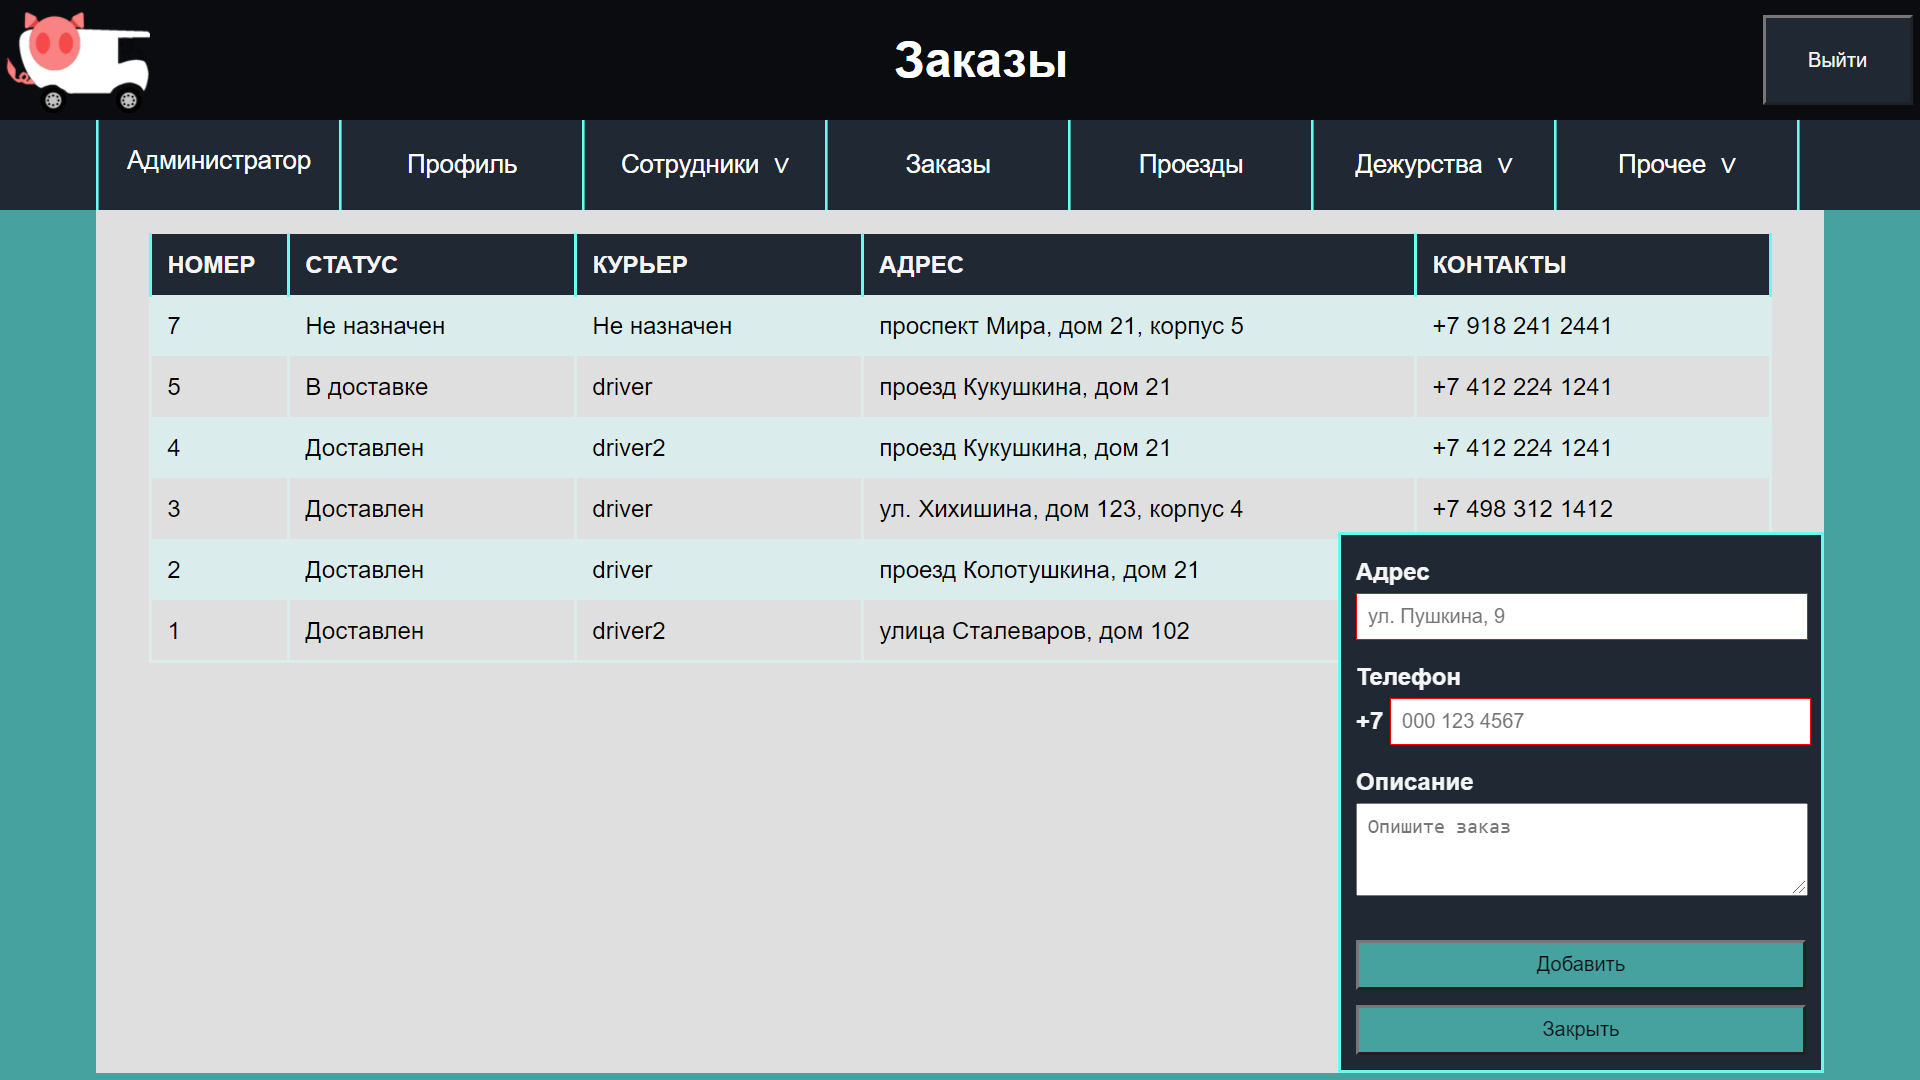
\includegraphics[scale=0.43, angle=0]{sc/all_delivery}}
		\caption{Страница просмотра и создания заказов}
		\label{sc:all_delivery}
	\end{center}
\end{figure}

Вышеупомянутая страница подробной информации о заказе приведена на рисунке \ref{sc:pick_delivery}. Страница доступна для водителей и администраторов. Обе роли могут поручить заказ водителю и завершить заказ. Администратор назначает водителя указанием его логина в всплывающем окне. Водитель способен назначить заказ только себе нажатием кнопки <<Выбрать заказ>>.
\begin{figure}[h!] 
	\begin{center}
		%		{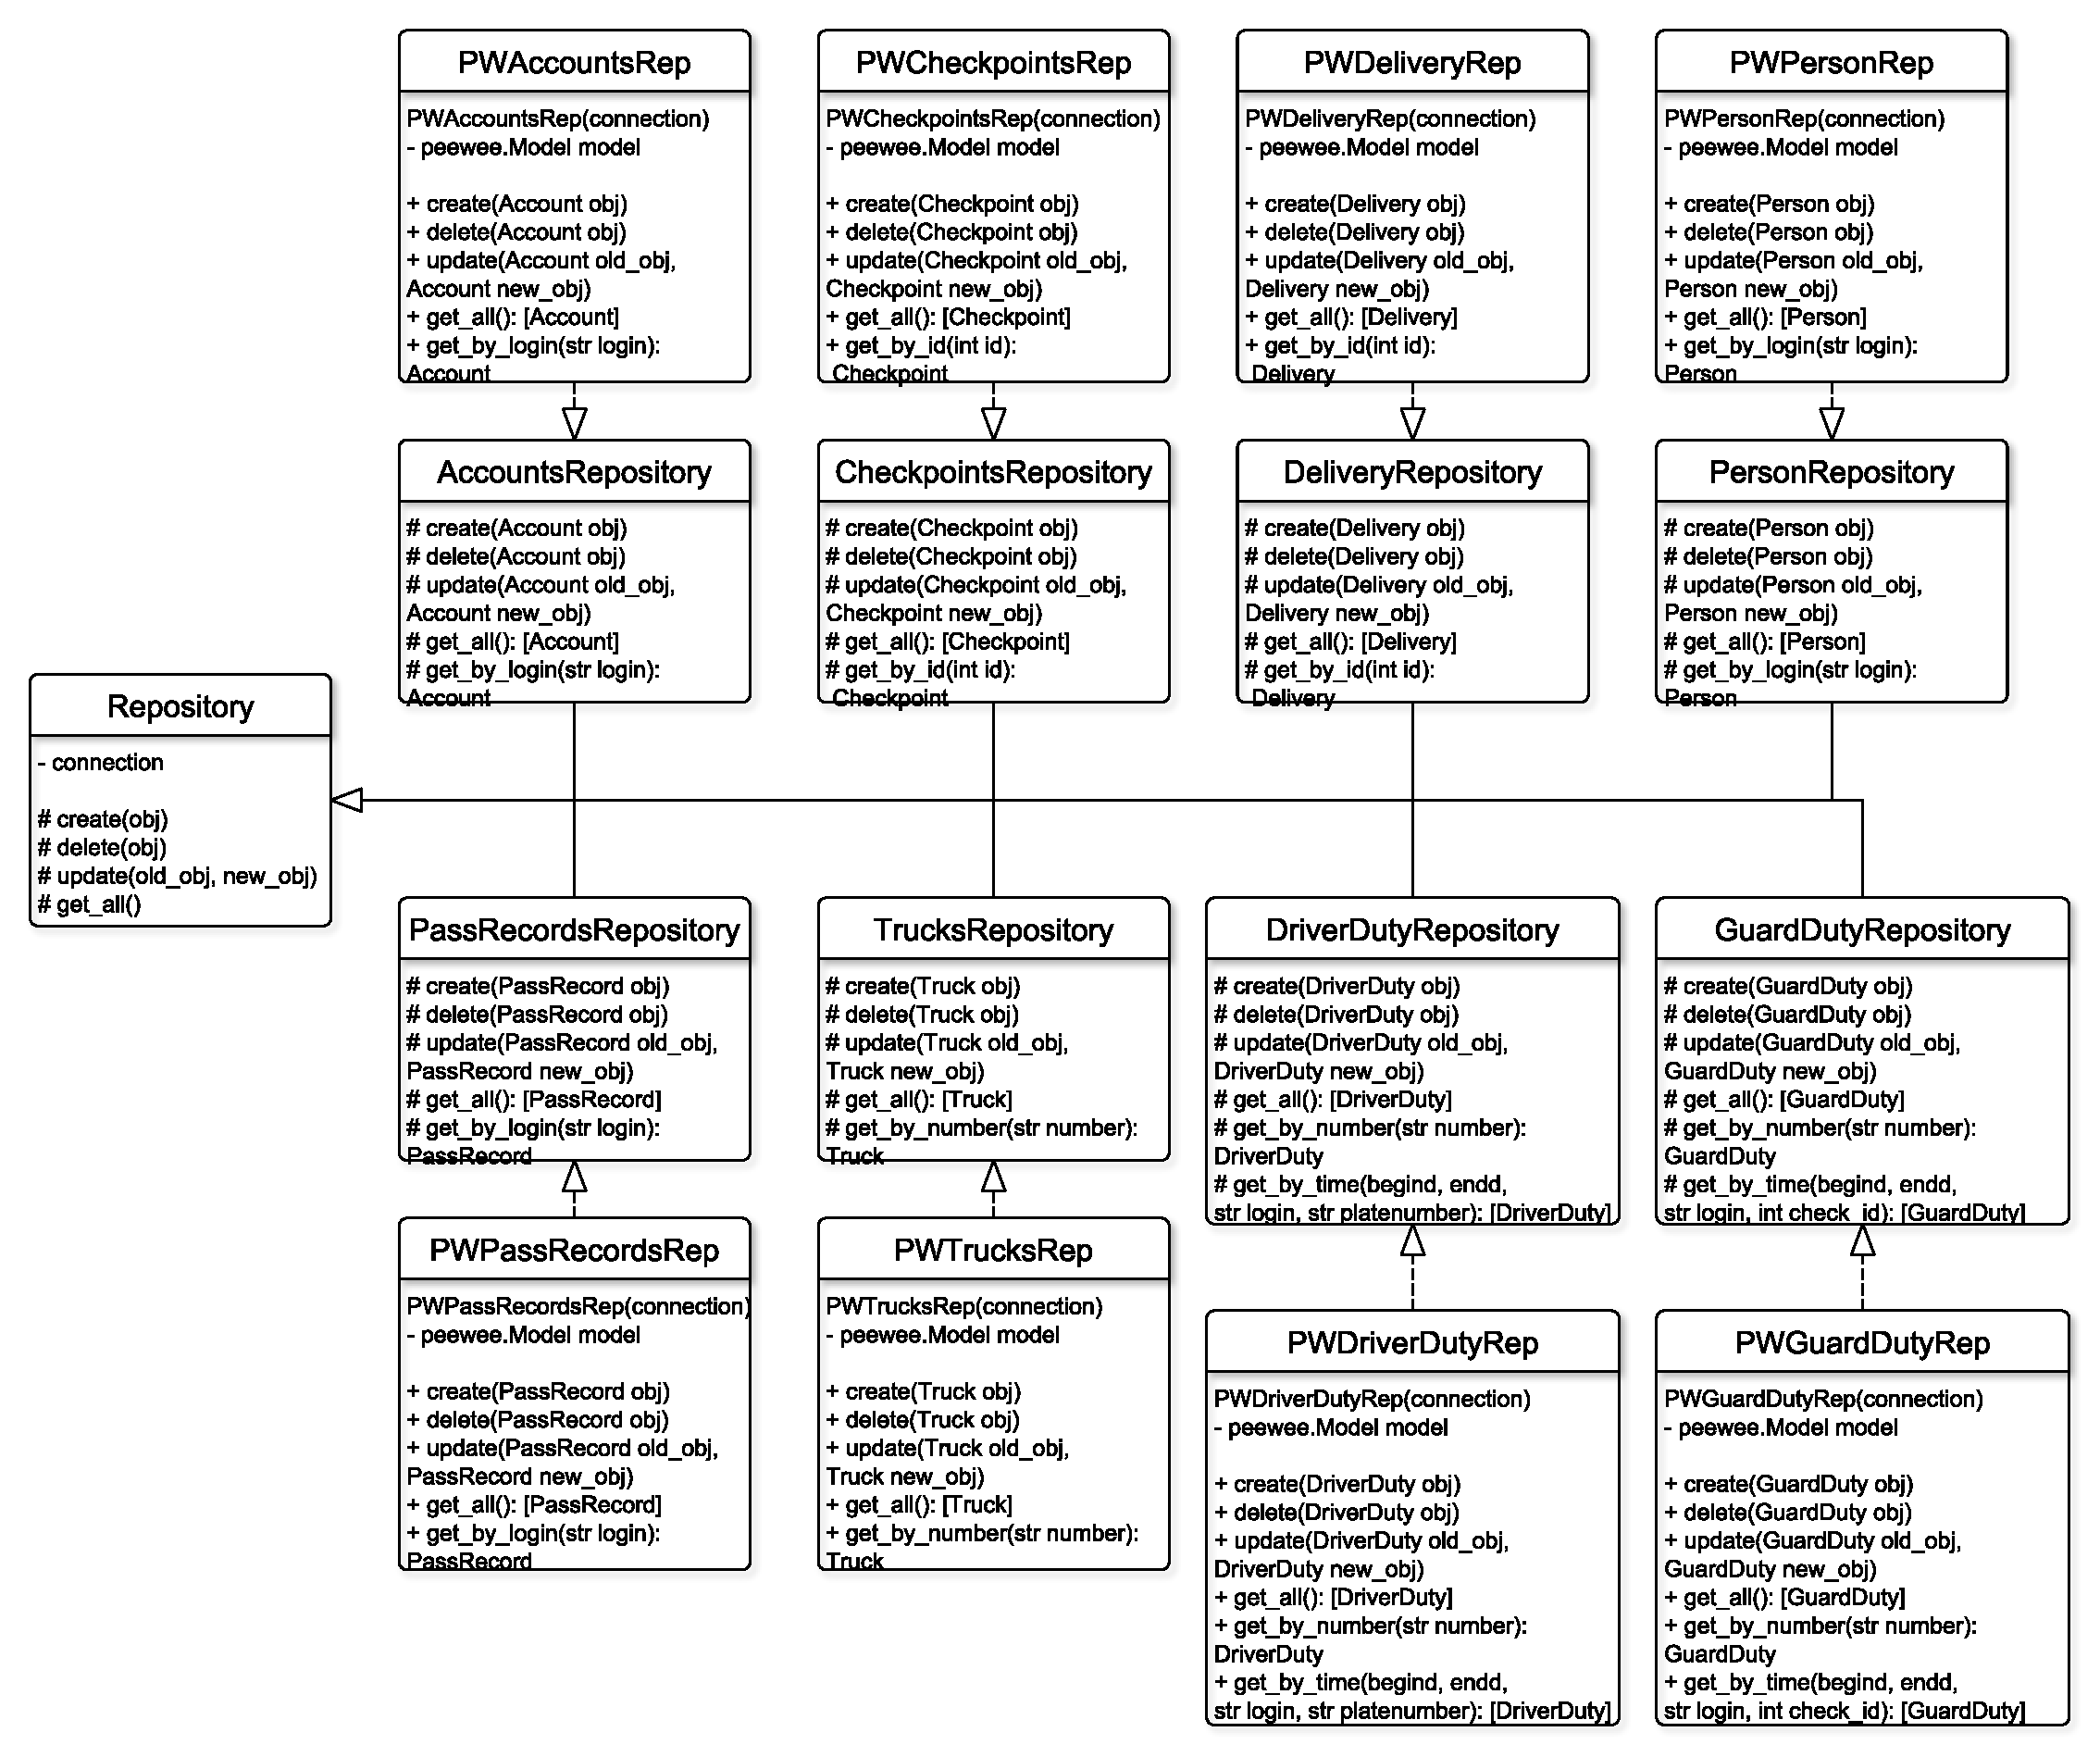
\includegraphics[height=14cm, width = 14cm]{uml/repsoitory.pdf}}
		{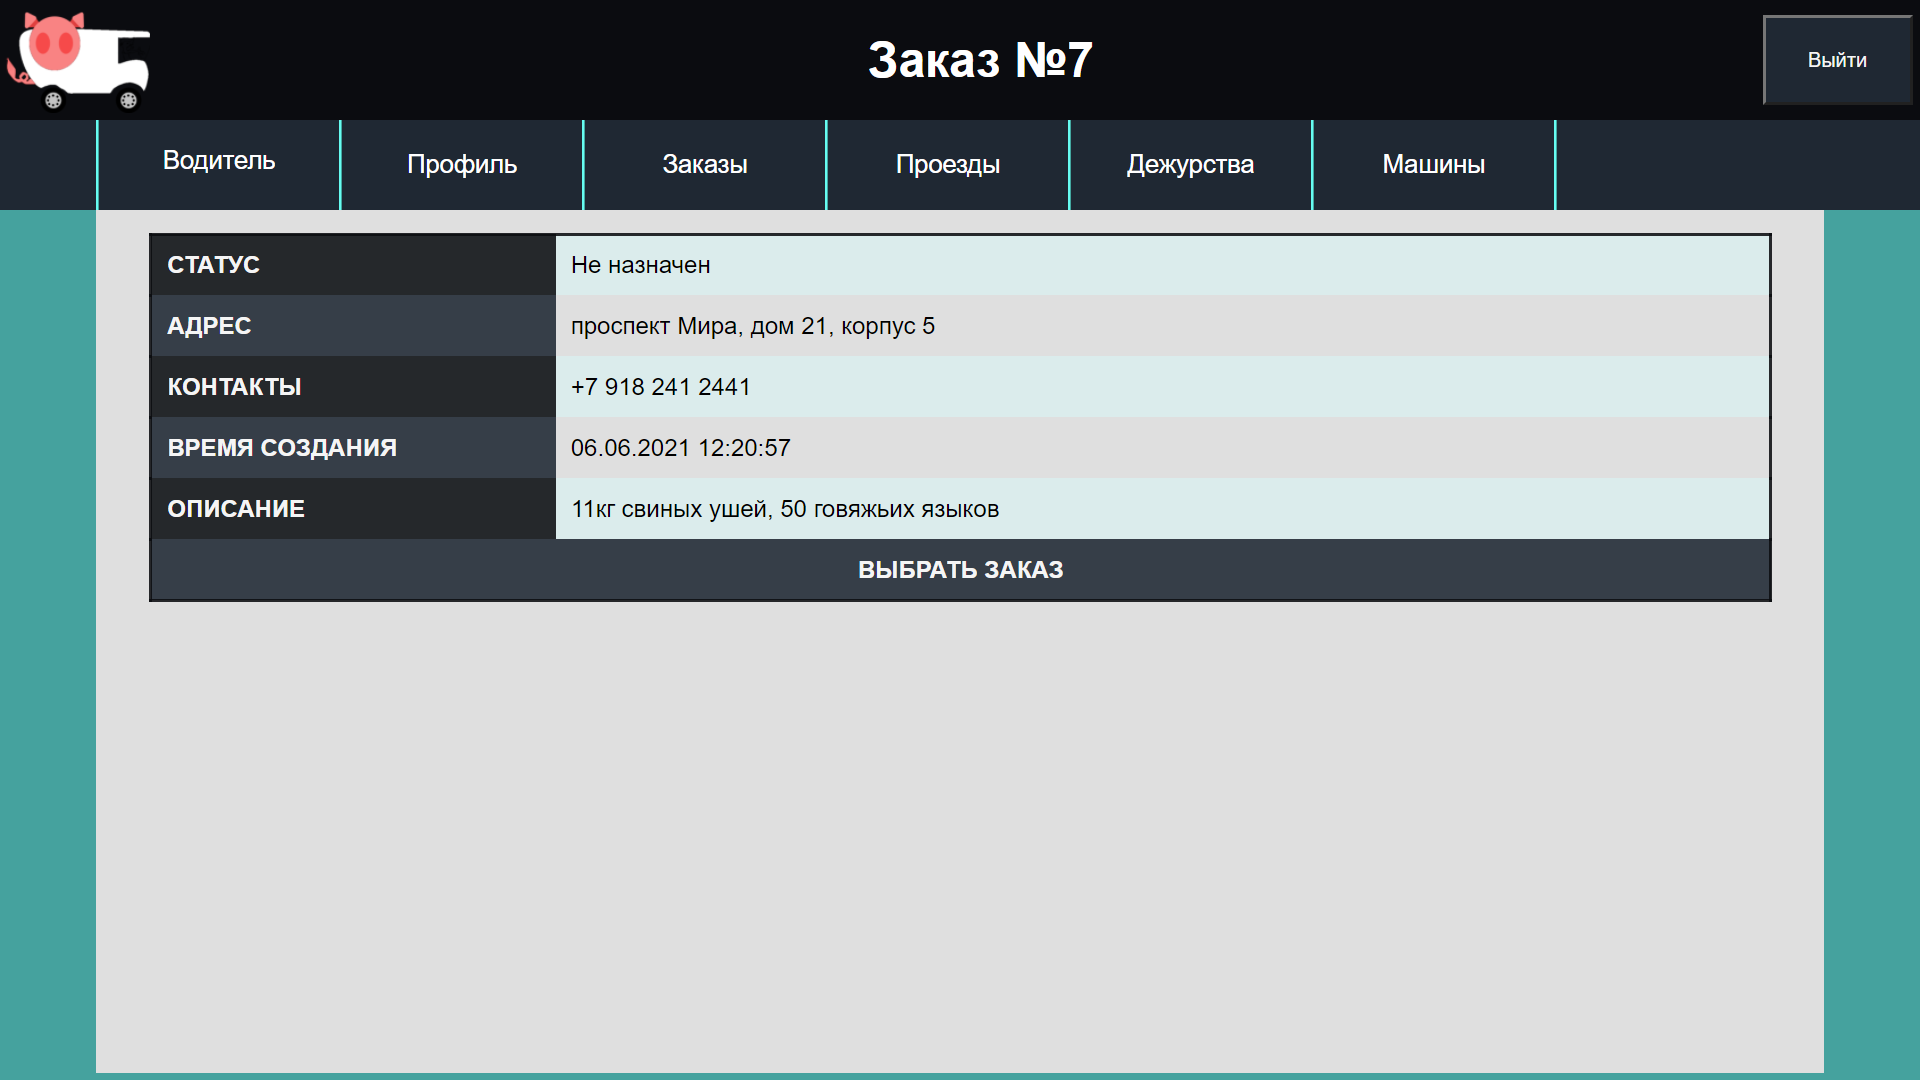
\includegraphics[scale=0.45, angle=0]{sc/pick_delivery}}
		\caption{Страница просмотра и выбора заказа (для роли водителя)}
		\label{sc:pick_delivery}
	\end{center}
\end{figure}

На рисунке \ref{sc:all_pass} изображена страница всех записей проездов. Для администратора на данной странице выводятся все записи в обратном хронологическом порядке и окно для добавления новой записи. Для охранника на данной странице видны записи о проезде в пределах его текущего дежурства (т.е. через определённое КПП в ограниченный временной диапазон). Охранник также может добавить запись о проезде, но в отличие от администратора ему не нужно указывать номер КПП.

\begin{figure}[h!] 
	\begin{center}
		%		{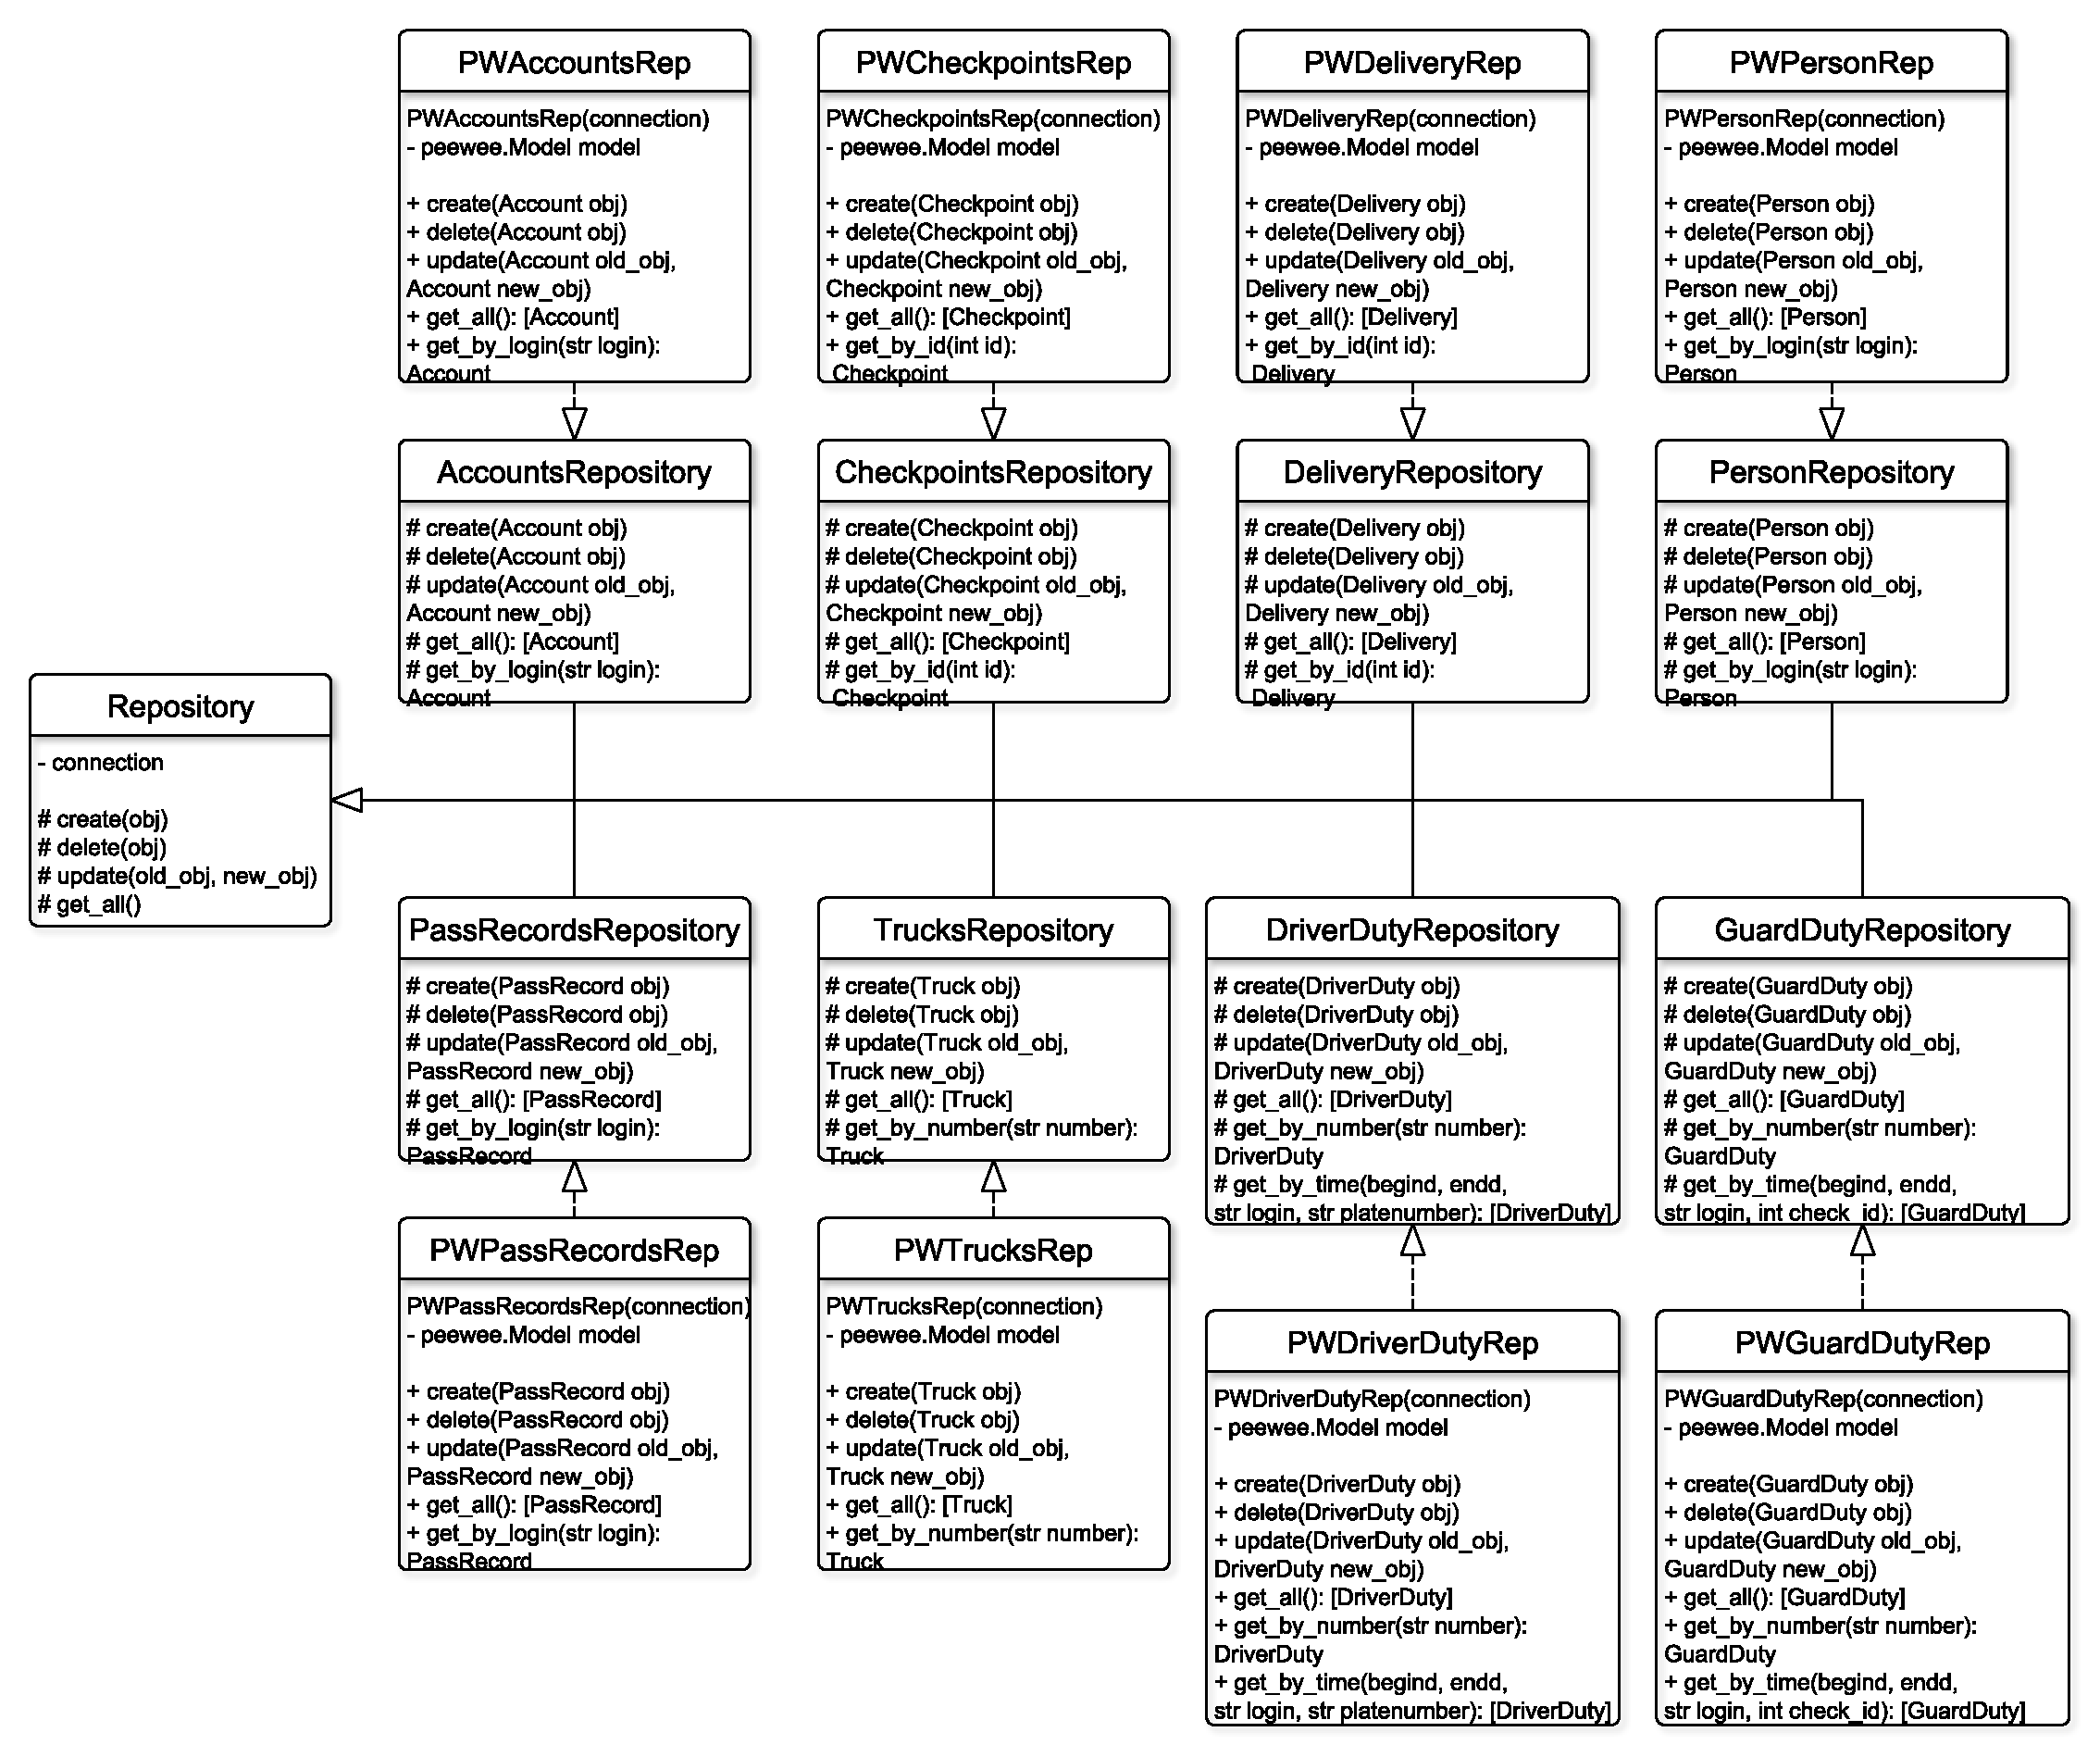
\includegraphics[height=14cm, width = 14cm]{uml/repsoitory.pdf}}
		{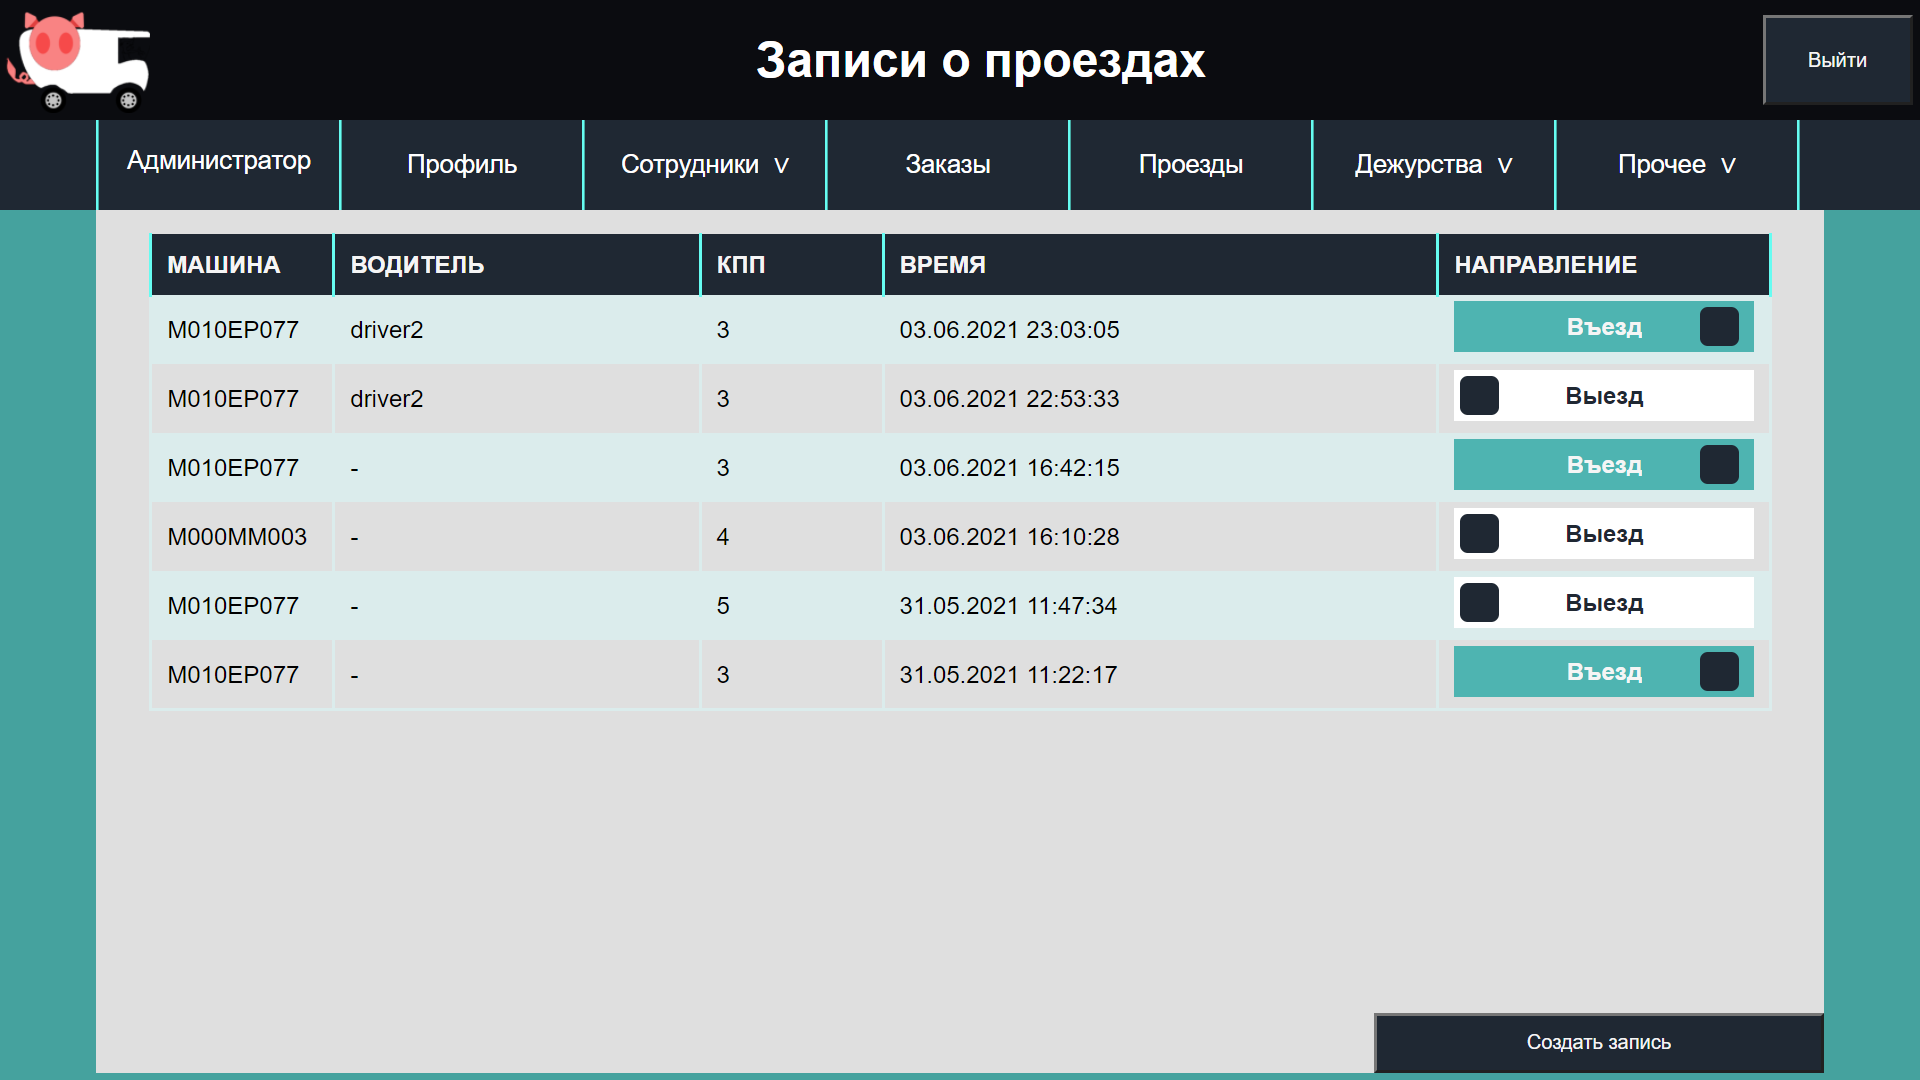
\includegraphics[scale=0.45, angle=0]{sc/all_pass}}
		\caption{Страница просмотра и регистрации записей о проездах}
		\label{sc:all_pass}
	\end{center}
\end{figure}

На следующем рисунке \ref{sc:driver_duty} представленна страница дежурств водителей. Доступ к ней имеют все подтверждённые сотрудники (охранники могут просматривать аналогичную страницу для их роли). Администратору выводятся все дежурства, отдельно отмечаются те, которые идут в данный момент. Также он может назначить новое дежурство в всплывающем окне. Для этого нужно указать логин сотрудника, номер КПП или машины (в зависимости от роли) и время его дежурства (задаётся диапазоном дат, времени и днями недели).  

Водители и охранники на этой странице могут видеть все свои дежурства и информацию о ближайшем из них.
\begin{figure}[h!] 
	\begin{center}
		%		{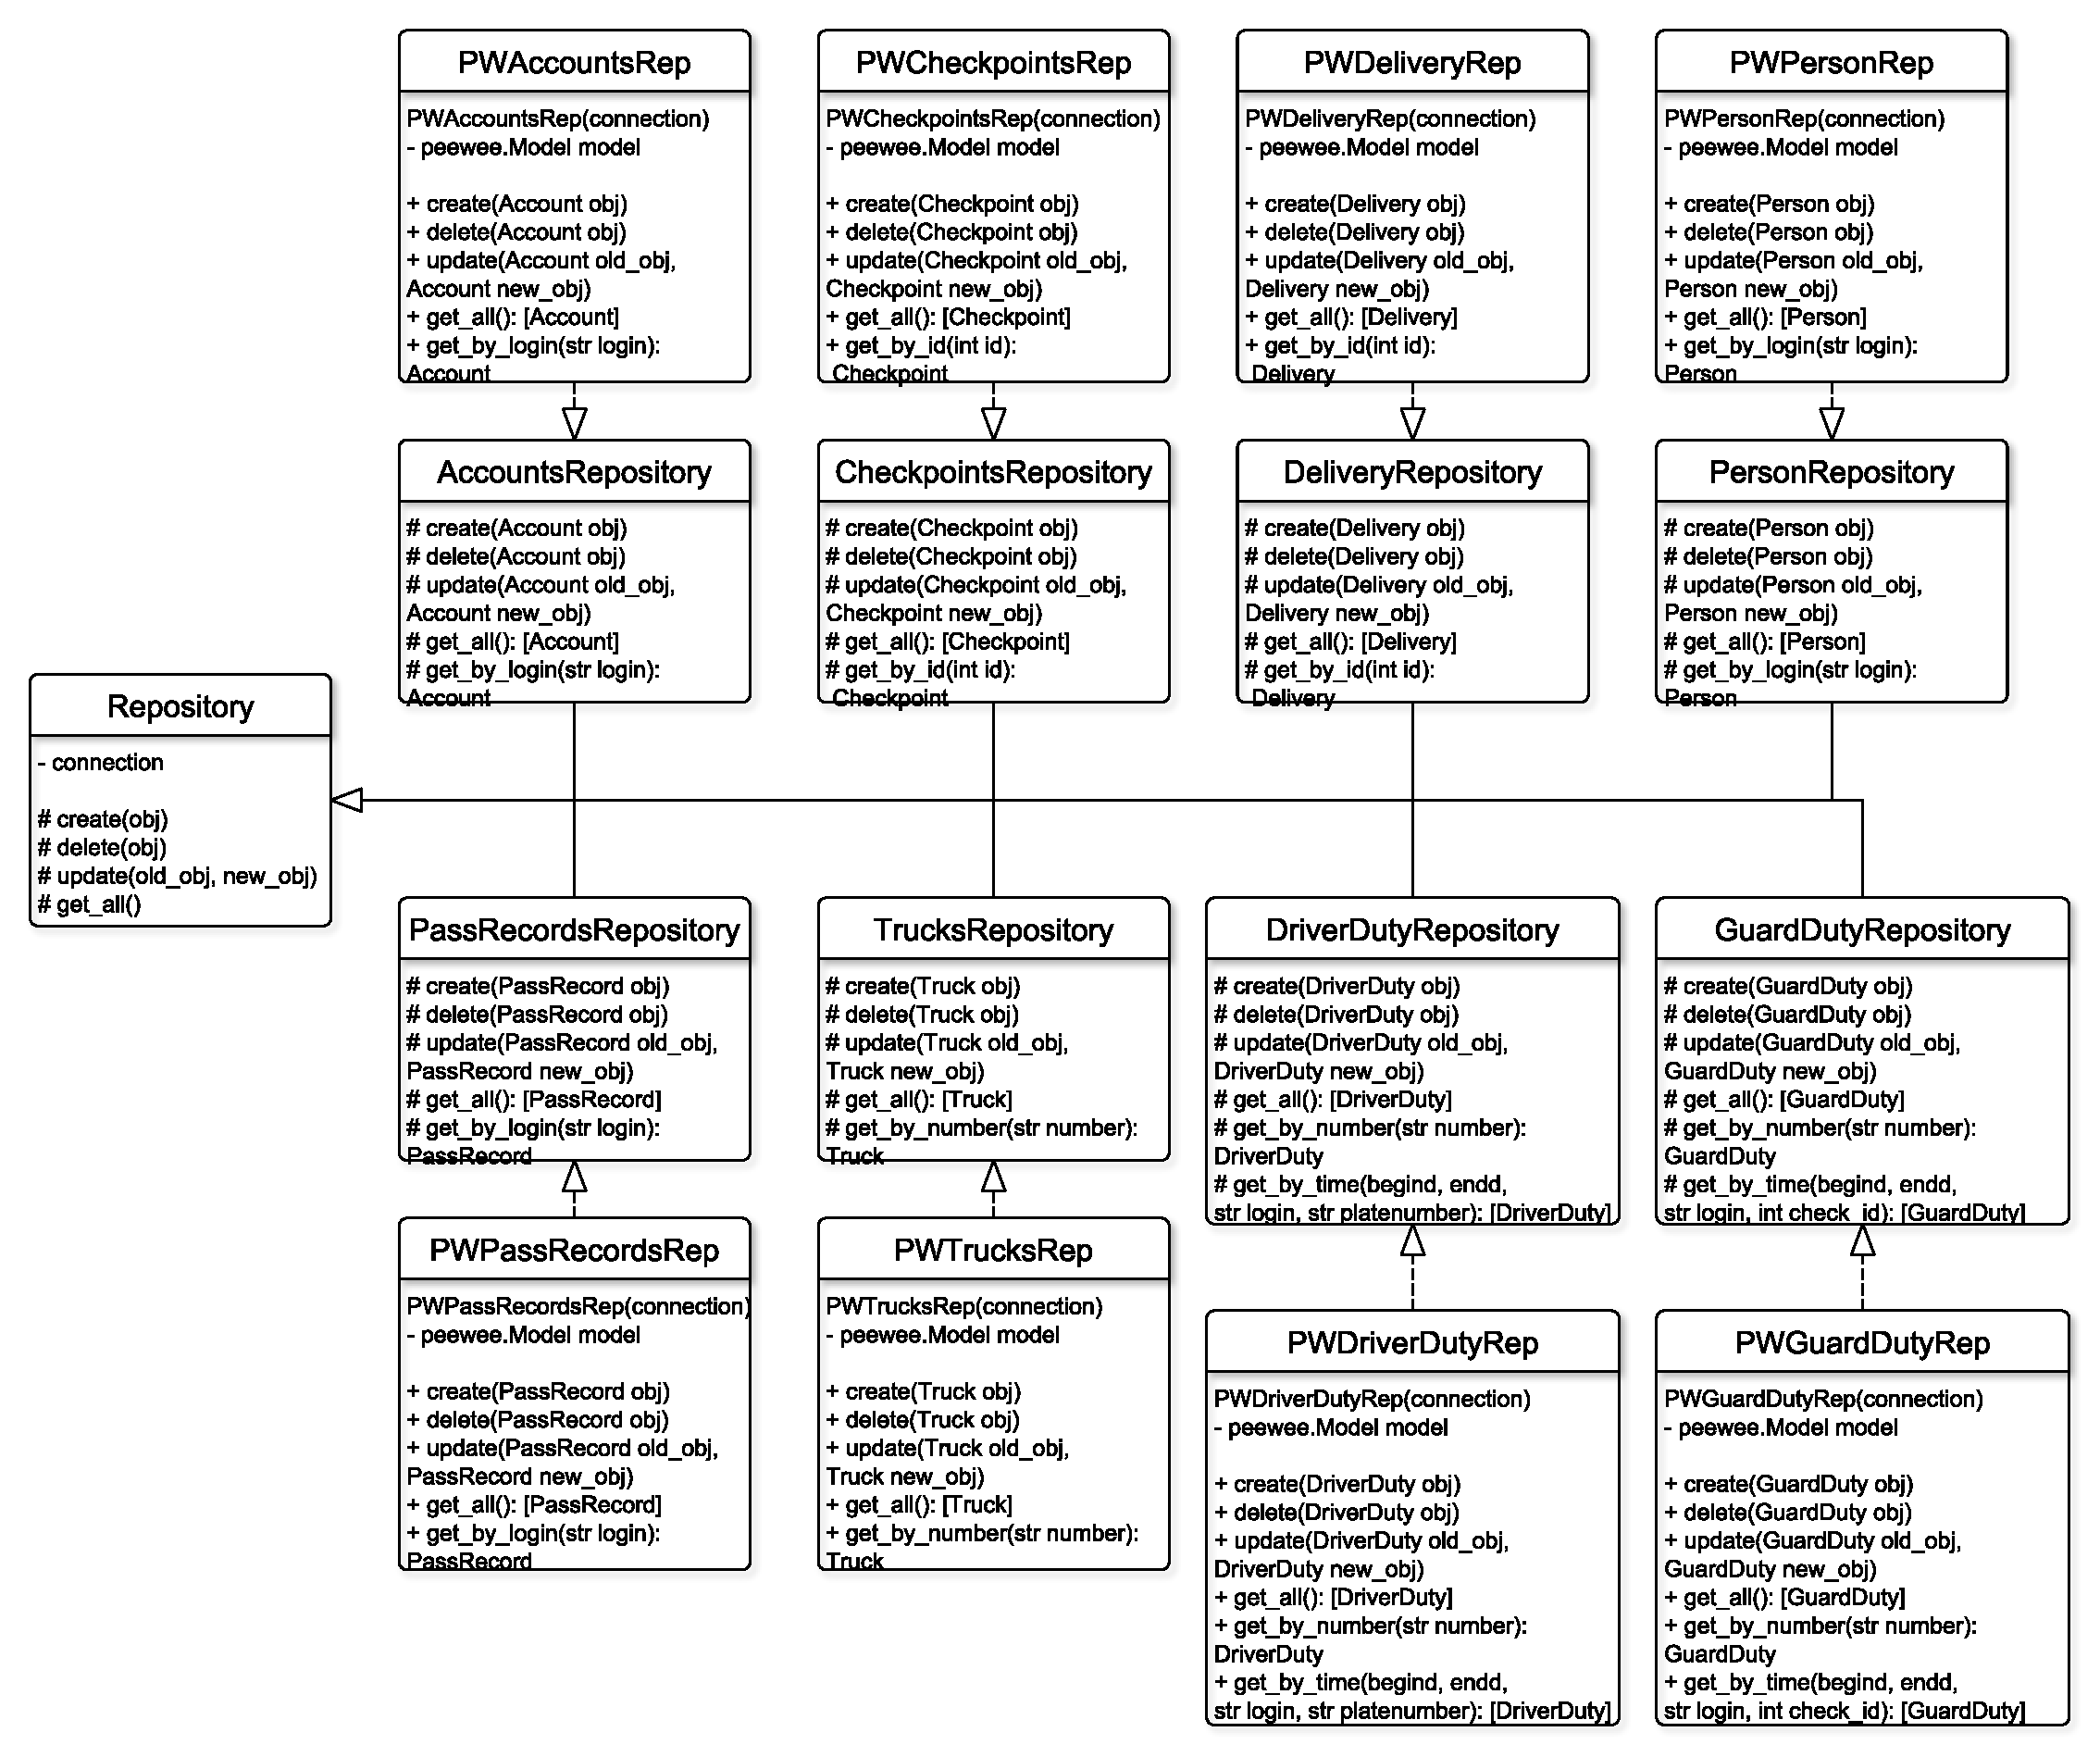
\includegraphics[height=14cm, width = 14cm]{uml/repsoitory.pdf}}
		{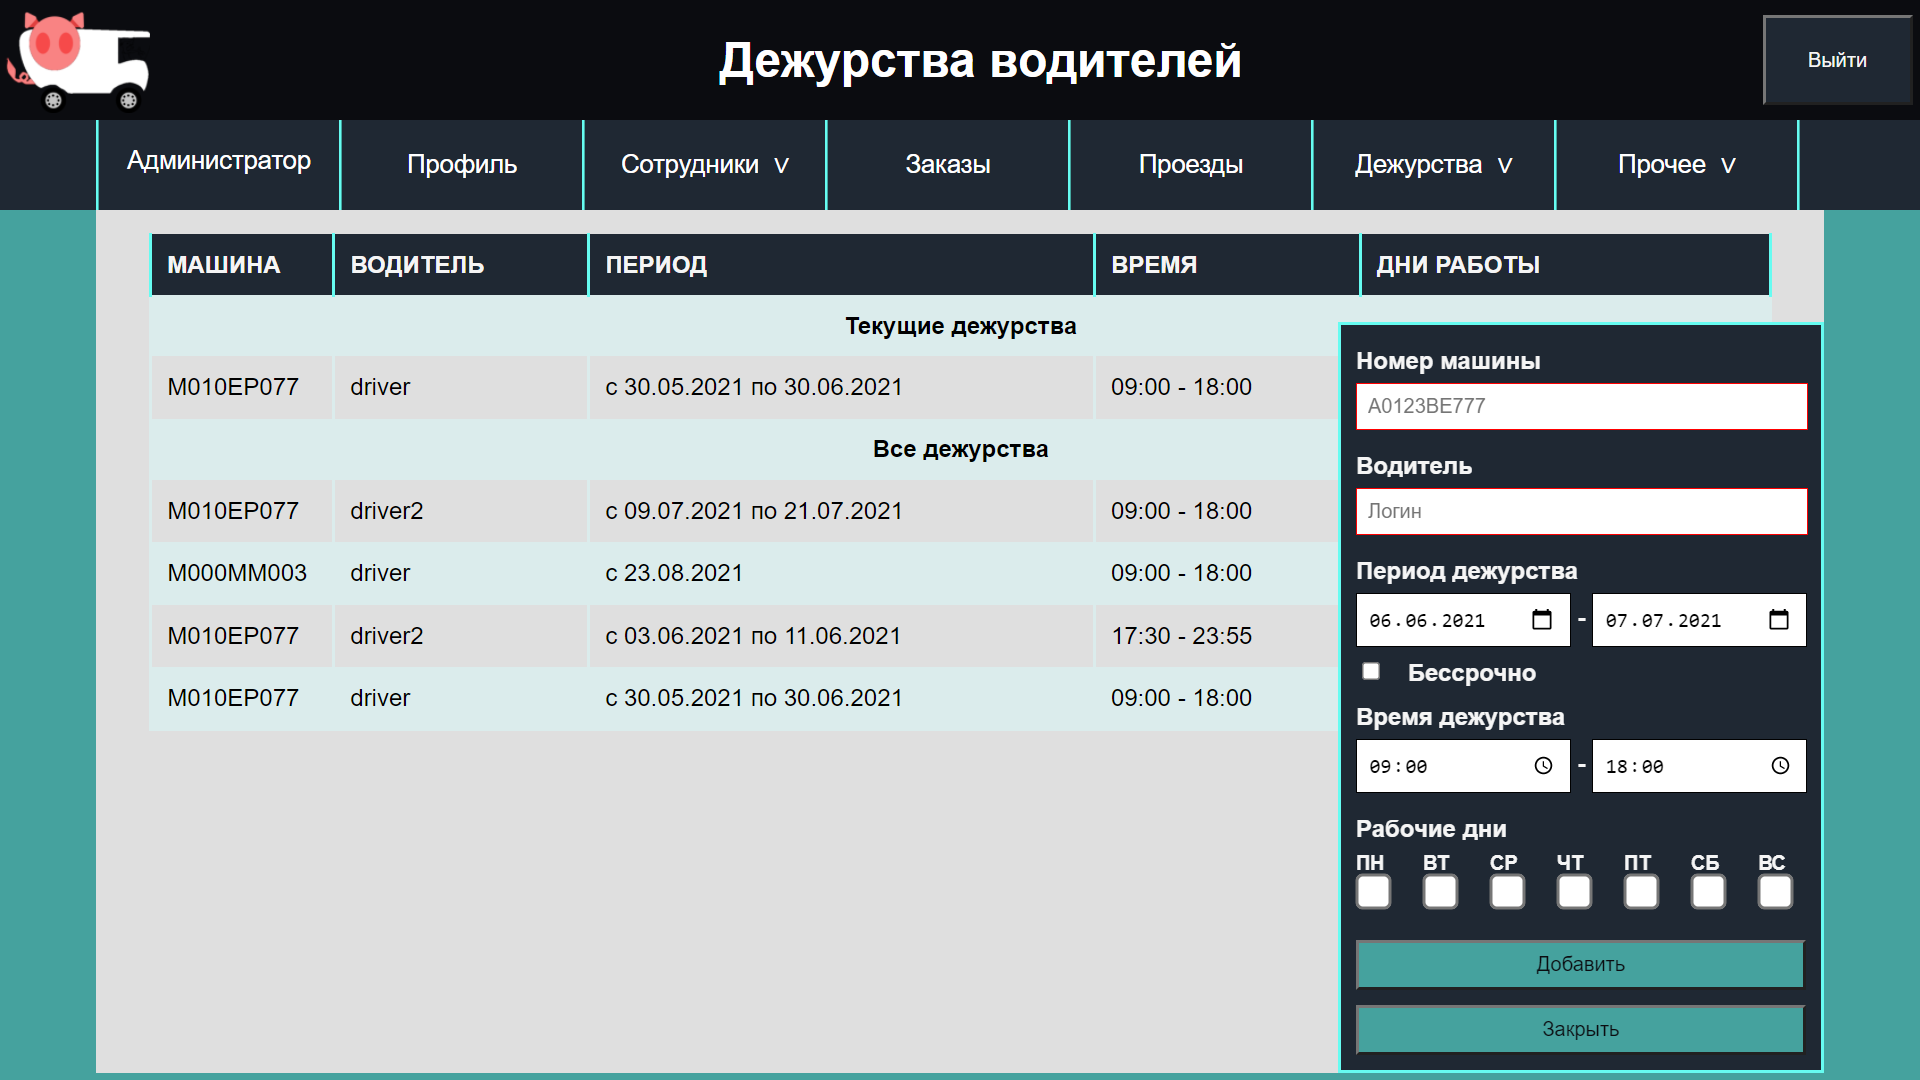
\includegraphics[scale=0.43, angle=0]{sc/driver_duty}}
		\caption{Страница просмотра и назначения дежурств водителей}
		\label{sc:driver_duty}
	\end{center}
\end{figure}

Также администратору доступны страницы просмотра и регистрации машин и КПП. На них представлен полный список данных объектов и всплывающее окно с формой добавления нового объекта.

Для неавторизованного пользователя доступны страницы входа в аккаунт и регистрации.

\section*{Вывод}
Результатом технологической части стал выбор средств программной реализации, реализация и описание структуры базы данных и приложения, визуальная демонстрация интерфейса приложения.
